\documentclass[phd,tocprelim]{cornell}
\let\ifpdf\relax
%
% tocprelim option must be included to put the roman numeral pages in the
% table of contents
%
% The cornellheadings option will make headings completely consistent with
% guidelines.
%
% This sample document was originally provided by Blake Jacquot, and
% fixed up by Andrew Myers.
%
%Some possible packages to include
\usepackage{graphicx,pstricks}
%\usepackage{graphics}
\usepackage{moreverb}
%\usepackage{epsfig}
\usepackage{subfigure}
\usepackage{hangcaption}
%\usepackage{txfonts}
\usepackage{palatino}
\usepackage{amsmath}
\usepackage{amsfonts}
\usepackage{multirow}
% For code lisitings
\usepackage{listings}
% URLs
\usepackage{hyperref}

%if you're having problems with overfull boxes, you may need to increase
%the tolerance to 9999
\tolerance=9999

\bibliographystyle{plain}
%\bibliographystyle{IEEEbib}

\renewcommand{\caption}[1]{\singlespacing\hangcaption{#1}\normalspacing}
\renewcommand{\topfraction}{0.85}
\renewcommand{\textfraction}{0.1}
\renewcommand{\floatpagefraction}{0.75}

\title {Hardware Architectures for Secure, Reliable, and Energy-Efficient Real-Time Systems}
\author {Daniel Lo}
\conferraldate {August}{2015}
\degreefield {Ph.D.}
\copyrightholder{Daniel Lo}
\copyrightyear{2015}

\begin{document}

\maketitle
\makecopyright

\begin{abstract}
The last decade has seen an increased ubiquity of computers with the widespread
adoption of smartphones and tablets and the continued spread of embedded
cyber-physical systems. With this integration into our environments, it has
become important to consider the real-world interactions of these computers
rather than simply treating them as abstract computing machines. For example,
cyber-physical systems typically have real-time constraints in order to ensure
safe and correct physical interactions. Similarly, even mobile and desktop
systems, which are not traditionally considered real-time systems, are
inherently time-sensitive because of their interaction with users.  Traditional
techniques proposed for improving hardware architectures are not designed with
these real-time constraints in mind. In this thesis, we explore some of the
challenges and opportunities in hardware design for real-time systems.
Specifically, we study recent techniques for improving security, reliability,
and energy-efficiency of computer systems. We analyze and adapt recently
proposed run-time monitoring techniques for improving security and reliability
to real-time systems. In addition, we show how to take advantage of dynamic
voltage and frequency scaling in the presence of timing requirements for
improved energy-efficiency.


\end{abstract}

\begin{biosketch}
Daniel Lo received his Bachelor of Science (with Honors) degree in Electrical
Engineering from the California Institute of Technology in 2009. Since then, he
has been a doctoral student at Cornell University pursuing a Doctor of
Philosophy in Electrical and Computer Engineering.
\end{biosketch}

% \begin{dedication}
% This thesis is dedicated to
% \end{dedication}

\begin{acknowledgements}
Your acknowledgements go here. Make sure it sits inside the brackets.
\end{acknowledgements}

\contentspage
\tablelistpage
\figurelistpage

\normalspacing \setcounter{page}{1} \pagenumbering{arabic}
\pagestyle{cornell} \addtolength{\parskip}{0.5\baselineskip}

\chapter{Introduction}
\label{chap:intro}

% Real-time systems are important
The last decade has seen an increased ubiquity of computers with the widespread
adoption of smartphones and tablets and the continued spread of embedded
cyber-physical systems. With this deep integration into our environments, it has
become important to consider the real-world interactions of these computers
rather than simply treating them as abstract computing machines. For example,
cyber-physical systems typically have real-time constraints in order to ensure
safe and correct physical interactions. Similarly, even mobile and desktop
systems, which are not traditionally considered real-time systems, are
inherently time-sensitive because of their interaction with users.
These real-time systems introduce new constraints and trade-offs for computer
systems design.

Real-time systems are typically specified as a set of tasks which have
real-time deadlines. Correct operation involves both correct computation of
outputs as well as finishing tasks before their deadlines.  Deadlines can
either be considered hard deadlines, where a missed deadline indicates a fatal
error, or soft deadlines, where a missed deadline results in poor performance
but is not fatal. Extensive work has been done in the software design and
analysis of real-time systems including real-time scheduling algorithms
\cite{rtschedulingsurvey-csur11}, real-time operating systems (RTOS)
\cite{rtossurvey-micro09, rtossurvey-icesc14}, and worst-case execution time
(WCET) analysis \cite{wcetsurvey-tecs08}.

% Thesis statement
In order to guarantee that deadlines are met, these systems are typically
designed conservatively so that even in the worst-case tasks will not exceed
their deadlines. As a result, in the average or typical case, tasks finish
before their deadline. This results in unused slack time between the task
finish and the deadline. One option to reclaim this unused time is to use it
for non-real-time (e.g., best effort) tasks. In this thesis, we explore the
software/hardware co-design of real-time systems in order to take advantage of
slack using modern hardware features. Specifically, we explore two angles for
improving computer systems. First, we explore the use of modern hardware
techniques for improving system security and reliability in the context of
real-time deadlines. Second, we take advantage of slack time to improve energy
efficiency by adjusting hardware resource allocations.

% Thesis statement
%On the other hand, traditional techniques proposed for improving
%hardware architectures are only evaluated for their average-case
%performance and are not designed to take into account the possibility of timing
%constraints. This thesis explore the development of hardware
%architectures that are aware of real-time requirements. Specifically, 
%we present solutions for applying modern hardware techniques for improving
%system security, reliability, and energy-efficiency to real-time systems.

\section{Secure and Reliable Hardware Architectures for Real-Time Systems}
\label{sec:intro.security}

% Run-time monitoring is useful
One potential use of extra time is for improving system security and
reliability by monitoring and checking run-time behavior.
Run-time monitoring techniques have been shown to be useful for improving the
reliability, security, and debugging capabilities of computer systems. For
example, Hardbound is a hardware-assisted technique to detect out-of-bound
memory accesses, which can cause undesired behavior or create a security
vulnerability if uncaught \cite{hardbound-asplos08}. Intel has recently
announced plans to support buffer overflow protection similar to Hardbound in
future architectures \cite{intel-mpx}. Similarly, run-time monitoring can
enable many other new security, reliability, and debugging capabilities such as
fine-grained memory protection \cite{mondrian-asplos02}, information flow
tracking \cite{dift-asplos04, testudo-micro08}, control flow integrity checking
\cite{hafix-dac15}, hardware error detection \cite{argus-micro07}, data-race
detection \cite{radish-isca12, cord-hpca06}, etc.  
However, today's parallel monitoring techniques cannot be easily applied
to critical real-time systems due to their lack of timing guarantees. Thus, we
have developed several techniques in order to enable run-time monitoring on
real-time systems.

% Parallel programmable monitoring
%There are several options on how to implement run-time monitoring.
%Implementing run-time monitoring in software using binary instrumentation or
%other similar methods introduces especially high overheads. For example,
%dynamic information flow tracking (DIFT) implemented in software suffers a 3.6x
%slowdown on average \cite{qin06-lift}. Implementing monitors in hardware
%greatly decreases the performance impact by performing monitoring in parallel
%to a program's execution. A dedicated hardware implementation of DIFT reduces
%average performance overheads to just 1.1\% \cite{suh-dift-asplos04}.  However,
%fixed hardware loses the programmability of software. A fixed hardware
%implementation cannot be updated and cannot change the type of run-time
%monitoring performed. Thus, recent studies have proposed using programmable
%parallel hardware, such as extra cores in a multi-core system or FPGA
%coprocessors, for monitoring \cite{chen08-lba, flexcore-micro10,
%harmoni-dsn12}. Our work in this paper is targeted at these programmable
%parallel hardware monitors.

% Monitoring WCET
Traditional real-time systems design requires estimation of the worst-case
execution time of tasks in order to guarantee schedulability. Thus, we first
developed a static analysis method to estimate the worst-case execution time
(WCET) impact of parallel run-time monitoring for real-time systems
(Chapter~\ref{chap:monitoring_wcet}). This allows run-time monitoring to be
enabled if there is enough static slack in a real-time system's schedule.
Our analysis works by extending the traditional integer-linear programming
(ILP) formulation used for estimating WCET by adding new constraints in order
to model the impact of run-time monitoring.

% Monitoring Hard Drop
Slack exists not only in the real-time schedule (i.e., static slack) but also
at run-time due to tasks running faster than their deadline (i.e., dynamic
slack). In order to take advantage of this dynamic slack for security and
reliability, we developed a hardware architecture that selectively performs
monitoring while guaranteeing that deadlines are met
(Chapter~\ref{chap:monitoring_hard_drop}). The architecture dynamically enables
or disables monitoring in order to meet real-time deadlines.

% Monitoring Soft Drop
Finally, soft real-time and interactive systems do not require strict timing guarantees
but still look to achieve timely execution of programs. Thus, by building on
our work in applying monitoring to hard real-time systems, we created an
architecture that enables adjustable overheads by trading off monitoring coverage
(Chapter~\ref{chap:monitoring_dift_drop}). 

\section{Energy-Efficient Hardware Architectures for Real-Time Systems}
\label{sec:intro.energy}

For modern mobile and embedded systems, energy usage is a major concern due to
limited battery life. Techniques, such as dynamic frequency and voltage scaling
(DVFS) and heterogeneous core mixes, have been developed to enable a trade off
between power and performance. These resource allocation techniques can be used
to reduce energy usage at the cost of increased execution time.

Traditional managers for these resource allocation techniques, such as DVFS,
work in a best effort manner. They operate under the assumption that better
performance is desired and only attempt to decrease resources when the
performance impact is minimal.  However, many applications or jobs have
response-time deadlines. Finishing faster than this response-time
requirement has no benefit. For example, responding to a user input faster than
human reaction time does not improve user experience. Similarly, decoding video
frames faster than the video frame rate has no added benefit. 

For these soft real-time systems, we can take advantage of this slack in order
to save energy without impacting user experience. In this thesis, we present a
method to predict the appropriate DVFS operating point for tasks in order to
meet deadlines with minimal energy (Chapter~\ref{chap:exec_time_prediction}).
This prediction needs to take into account the effect of inputs and program
state in order to account for dynamic variations in task execution time. We
show how this is possible through static analysis of task source code in order
to generate task-specific predictors for DVFS control.

\section{Organization}
The rest of the thesis is organized as follows.
Chapter~\ref{chap:background} discusses some background knowledge and
terminology that will be used throughout the thesis.
Chapters~\ref{chap:monitoring_wcet}, \ref{chap:monitoring_hard_drop}, and
\ref{chap:monitoring_dift_drop} discuss our work on improving system security
and reliability through run-time monitoring on real-time systems. 
%Chapter~\ref{chap:monitoring_wcet} discusses the static analysis of run-time
%monitoring for hard real-time systems. Chapter~\ref{chap:monitoring_hard_drop}
%describes a dynamic scheme for implementing run-time monitoring on hard
%real-time systems. Chapter~\ref{chap:monitoring_dift_drop} extends this schemes
%to other applications with soft rather than hard deadlines.
Chapter~\ref{chap:exec_time_prediction} presents our work on creating
energy-efficient real-time systems. Finally, Chapter~\ref{chap:related_work}
discusses related work and Chapter~\ref{chap:conclusion} concludes the thesis.

\chapter{WCET Analysis of Run-Time Monitoring}
\label{chap:monitoring_wcet}

\section{Introduction}
\label{sec:monitoring_wcet.introduction}

In order to apply parallel run-time monitoring to traditional real-time systems, we must
be able to analyze the worst-case execution time (WCET) of running a program
with run-time monitoring. The only existing way to do this is to assume that
monitoring is done sequentially. However, this bound is overly conservative when used to analyze parallel run-time monitoring.
In this chapter, we present a method for estimating the increase in WCET of
programs running on a system with parallel monitoring. We first investigate how
to mathematically model the loosely-coupled relationship between the main 
processing core and parallel monitoring hardware, which are connected
through a FIFO buffer with a fixed number of entries. The resulting model
is non-linear but can be transformed into a mixed integer linear programming (MILP) 
formulation.
The MILP formulation produces the maximum number of cycles for each basic block
that the main core may be stalled due to monitoring.
These monitoring stalls can be incorporated into popular
WCET analysis methods based on implicit path enumeration techniques (IPET)
\cite{li-ipet-dac95} in order to estimate the WCET of tasks with run-time monitoring.

The rest of this chapter is organized as follows.
%Section~\ref{sec:monitoring_wcet.monitoring} gives an overview of the run-time
%monitoring architecture that we assume in this thesis.
Section~\ref{sec:monitoring_wcet.wcet} explains our MILP-based formulation for
estimating WCET and Section~\ref{sec:monitoring_wcet.example} provides an
example MILP formulation. Finally, Section~\ref{sec:monitoring_wcet.evaluation}
shows our evaluation results.



\section{WCET Analysis}
\label{sec:monitoring_wcet.wcet}

\subsection{Implicit Path Enumeration}
\label{sec:formulation:ipet}

Most of the WCET analysis techniques today rely on an ILP formulation that is
obtained from implicit path enumeration techniques \cite{li-ipet-dac95}.  In
this method, a program is converted to a control flow graph (CFG). From the
control flow graph, an ILP problem is formulated that seeks to maximize
\begin{align*}
  t = \sum_{B \in \mathcal{B}_{CFG}}{N_B \cdot c_{B,max}}
\end{align*} 
where $\mathcal{B}_{CFG}$ is the set of basic blocks in the control flow graph.
$N_{B}$ is the number of times block $B$ is executed and $c_{B,max}$ is the
maximum number of cycles to execute block $B$. The maximum value of $t$ is the
WCET of the task.  To account for the fact that only certain paths in the graph
will be executed, a set of constraints are placed on $N_{B}$. For example, on a
branch, only one of the branches will be taken on each execution of the block.
A variable can be assigned to each edge corresponding to the number of times
that edge is taken.  The number of times edges out of the block are taken must
equal the number of times the block is executed.  Similarly, the number of
times edges into the block are taken must equal the number of times the block
is executed. Various methods have been developed to create additional
constraints to convey other program behavior \cite{li-ipet-dac95,
wcetsurvey-tecs08}.

%% Why ILP?
Integer linear programming is an attractive optimization technique for this
problem because the solution found is a global optimum. In addition, many
aspects of program and architecture behavior can be described by adding
constraints to the ILP problem.  Several open source and commercial ILP solvers
exist which can solve the formulated ILP problem \cite{lpsolve, cplex}.  Thus,
in developing a method for estimating the WCET of parallel run-time monitoring,
we look to build upon this ILP framework.

%% Using worst case stalls in original WCET analysis to determine WCET with monitoring.
The IPET-based ILP formulation can be extended in a straightforward fashion to
incorporate run-time monitoring overheads if we have the maximum (worst-case)
monitoring stall cycles for each basic block by maximizing
\begin{align*}
  t = \sum_{B \in \mathcal{B}_{CFG}}{N_{B} \cdot (c_{B,max} + s_{B,max})}
\end{align*}
Here, $s_{B,max}$ represents the maximum number of cycles that block $B$ is
stalled due to monitoring. In this sense, the challenge in WCET analysis with
monitoring lies in determining $s_{B,max}$.  The rest of this section addresses
this problem.

\subsection{Sequential Monitoring Bound}
\label{sec:formulation:sequential}

One way to determine a conservative bound on the worst-case monitoring stall
cycles is to consider sequential monitoring.  In sequential monitoring, the
monitoring task is run in-line with the main task on the same core rather than
in parallel. That is, after each instruction that would be forwarded, the
monitoring task is run on the main core before the main task resumes execution.
In this case, the WCET estimate can be obtained from a traditional method by
analyzing one program that contains both main and monitoring tasks.  The
resulting WCET can be considered as a simple bound for parallel monitoring
because it models the case where every forwarded instruction causes the main
core to stall.  However, this bound is extremely conservative as it does not
account for the FIFO buffering or the parallel execution of the monitoring
core. These features are critical to utilizing run-time monitoring techniques
while maintaining low performance overheads.

\subsection{FIFO Model}
\label{sec:formulation:model}

To obtain tighter WCET bounds, we need to model the FIFO.  The main task can
continue its execution as long as a FIFO entry is available, but needs to stall
on a forwarded instruction if the FIFO is full. The WCET model needs to capture
the worst-case (maximum) number of entries in the FIFO at each forwarded
instruction and determine how many cycles the main task may be stalled due to
the FIFO being full. Here, we propose a mathematical model to express the load
in the FIFO and estimate the worst-case stalls.

In this approach, the original control flow graph must be transformed so that
each node contains at most one forwarded instruction which is located at the
end of the code sequence represented by the node.  This transformed graph is
called a {\em monitoring flow graph (MFG)}.  Intuitively, the analysis needs to
consider one forwarded instruction at a time in order to model the FIFO state
on each forwarded instruction and capture all potential stalls from monitoring. 

To model how full the FIFO is, we define the concept of \emph{monitoring load}.
The monitoring load is the number of cycles required for the monitoring core to
process all outstanding entries in the FIFO at a given point in time. The
monitoring load increases when a new instruction is forwarded by the main task,
and decreases as the monitoring core processes forwarded instructions. For
simplicity, the increase in monitoring load for any forwarded instruction is
conservatively assumed to be the worst-case (maximum) monitoring task execution
time among all possible forwarded instructions. This maximum, $t_{M, max}$, can
be obtained from the WCET analysis of the monitoring tasks.  We make this
simplification because it is difficult to model the FIFO mathematically at an
entry-by-entry level. With this simplification, each FIFO entry is identical
and so the monitoring load fully represents the state of the FIFO.  The
monitoring load cannot be negative and is upper-bounded by the maximum
monitoring load the FIFO can handle, $l_{max}$. The maximum monitoring load is
the number of FIFO entries, $n_F$, multiplied by the increase in monitoring
load for one forwarded instruction, $t_{M, max}$.

In order to find the worst-case monitoring stalls, we need to determine the
worst-case (maximum) monitoring load at the node boundaries in the MFG. For a
given node, $M$, in the MFG, we define $li_{M}$ as the monitoring load coming
into the node and $lo_{M}$ as the monitoring load exiting the node. The change
in monitoring load for the node is denoted by $\Delta l_{M}$. The maximum
$\Delta l_{M}$ can be calculated as the difference between the WCET of a
monitoring task that corresponds to $M$ and the minimum execution cycles of the
node, $c_{M,min}$: 
\begin{align*}
\Delta l_{M} = 
	\begin{cases}
	t_{M,max} - c_{M,min}, &\text{forwarded inst. } \in M \\
	- c_{M,min}, &\text{no forwarded inst. } \in M
	\end{cases}
\end{align*}
In order to ensure that the analysis is conservative in estimating the
worst-case (maximum) stalls, we use the best-case (minimum) execution time for
the main task here. 

Because the monitoring load is bounded by zero and the maximum load that
the FIFO can handle, $l_{max}$, the monitoring load coming out of a node is
\begin{align*}
	lo_{M} =& 
		\begin{cases}
			0, &li_{M} + \Delta l_{M} < 0 \\
			li_{M} + \Delta l_{M}, &0 \leq li_{M} + \Delta l_{M} \leq l_{max} \\
			l_{max}, &li_{M} + \Delta l_{M} > l_{max}
		\end{cases} \\
  l_{max} =& n_F \cdot t_{M,max}
\end{align*}

The worst-case monitoring load entering node $M$, $li_{M}$, is the largest of
the output monitoring loads among nodes with edges pointing to node $M$. Let
$\mathcal{M_{\text{prev}}}$ represent the set of nodes with edges pointing to
node $M$. Then,
\begin{align*}
	li_{M} = \max_{M_{prev} \in \mathcal{M}_{prev}}lo_{M_{prev}}
\end{align*}

The above equations describe the worst-case monitoring load at each node
boundary.  A monitoring stall occurs when a forwarded instruction is executed
but there is no empty entry in the FIFO buffer. In terms of monitoring load, if
a node would add monitoring load that would cause the resulting total load to
exceed $l_{max}$, then a monitoring stall occurs. The number of cycles stalled,
$s_{M}$, is the number of cycles that this total exceeds $l_{max}$. That is,
\begin{align*}
	s_{M} =
		\begin{cases}
			0, &li_{M} + \Delta l_{M} < l_{max} \\
			(li_{M} + \Delta l_{M}) - l_{max}, &li_{M} + \Delta l_M \geq l_{max}
		\end{cases}
\end{align*}

These sets of equations describe the monitoring stalls for each node in the MFG.
The worst-case monitoring stall cycles can then be determined by maximizing the
value of each $s_M$. This is equivalent to a single objective of maximizing the
sum of the $s_M$,
\begin{align*}
  \max \sum_{M \in \mathcal{M}_{MFG}} s_{M}
\end{align*}
where $\mathcal{M}_{MFG}$ is the set of nodes in the MFG.  Once the worst-case
stalls for each MFG node is found, the worst-case stalls for a CFG node,
$s_{B,max}$, can be computed by simply summing the stalls from the
corresponding MFG nodes. We note that since the monitoring load is always
conservative in representing the FIFO state, no timing anomalies are exhibited
by this analysis. That is, determining the individual worst-case stalls results
in the global worst-case stalls.

\subsection{MILP Formulation}
\label{sec:formulation:milp}

The proposed FIFO model requires solving an optimization problem to obtain the
worst-case stalls, where the input and output monitoring loads, $li_{M}$ and
$lo_{M}$, and the monitoring stalls, $s_{M}$, need to be determined for each
node. Here, we show how the problem can be formulated using MILP. Although the
equations for $lo_{M}$ and $s_{M}$ are non-linear, they are piecewise linear.
Previous work has shown that linear constraints for piecewise linear functions
can be formulated using MILP \cite{sierksma-lp}. In the following constraints,
all variables are assumed to be lower bounded by zero unless otherwise
specified, as is typically assumed for MILP.

First, a set of variables, $lo'$ and $s'$, are created to represent the
unbounded versions of $lo$ and $s$. For readability, the per block subscript
$M$ has been omitted.
\begin{align*}
  s' =& li + \Delta l - l_{max}, \text{ } s' \in (-\infty, \infty)\\
  lo' =& li + \Delta l, \text{ } lo' \in (-\infty, \infty) 
\end{align*}
The following piecewise linear function calculates $s$ from $s'$.
\begin{align*}
  s = f(s') = 
    \begin{cases} 
    0, &s' < 0\\
    s', &s' \geq 0
    \end{cases}
\end{align*}
This function can be described in MILP using the following set of constraints.
\begin{align*}
  a_s\lambda_0 + b_s\lambda_2 =& s'\\
  \lambda_0 + \lambda_1 + \lambda_2 =& 1 \\
  \delta_1 + \lambda_2 \leq& 1 \\
  \delta_2 + \lambda_0 \leq& 1 \\
  \delta_1 + \delta_2 =& 1 \\
  b_s\lambda_2 =& s
\end{align*}
where $a_s$ is chosen to be less than the minimum possible value of $s'$ and
$b_s$ is chosen to be greater than the maximum possible value of $s'$. The
choice of $a_s$ and $b_s$ is arbitrary as long as it meets these requirements.
$\lambda_i$ are continuous variables and $\delta_i$ are binary variables. In
this set of constraints, $s'$ is expressed as a sum of the endpoints of a
segment of the piecewise function. The $\delta_i$ variables ensure that only
the segment corresponding to $s'$ is considered. $\delta_1 = 1$ corresponds to
the $s' < 0$ segment of $f(s')$ and $\delta_2 = 1$ corresponds to the $s' \geq
0$ segment of $f(s')$. The $\lambda_i$ variables represent exactly where $s'$
falls on the domain of that segment. $s$ can be calculated using this
information and the values of the function at the segment endpoints.

Similarly, $lo$ can be bound between $0$ and $l_{max}$ by using the following
set of constraints.
\begin{align*}
  a_l\lambda_3 + l_{max}\lambda_5 + b_l\lambda_6 =& lo'\\
  \lambda_3 + \lambda_4 + \lambda_5 + \lambda_6 =& 1 \\
  2 \delta_3 + \lambda_5 + \lambda_6 \leq& 2 \\
  2 \delta_4 + \lambda_3 + \lambda_6 \leq& 2 \\
  2 \delta_5 + \lambda_3 + \lambda_4 \leq& 2 \\
  \delta_3 + \delta_4 + \delta_5 = 1 \\
  l_{max}\lambda_5 + l_{max}\lambda_6 =& lo
\end{align*}
As before, $a_l$ and $b_l$ are chosen such that $lo' \in (a_l, b_l)$.  Again,
$\lambda_i$ are continuous variables and $\delta_i$  are binary variables.

Finally, for each node, the input monitoring load $li_{M}$ must be determined.
$li_{M}$ depends on the previous nodes, $\mathcal{M_\text{prev}}$. If there is
only one edge into the node, then $li_M$ is simply
\begin{align*}
  li_{M} = lo_{M_{prev}}
\end{align*}
When there is more than one edge into node $M$, one set of constraints is used
to lower bound $li_{M}$ by all $lo_{M_{prev}}$.
\begin{align*}
  li_{M} \geq& lo_{M_{prev}}, \text{ } \forall M_{prev} \in \mathcal{M_\text{prev}}
\end{align*}
Then, another set of constraints upper bounds $li_{M}$ by the maximum $lo_{M_{prev}}$.
\begin{align*}
  li_{M} - b \cdot \delta_{M_{prev}} \leq& lo_{M_{prev}}, \text{ } \forall M_{prev} \in \mathcal{M_\text{prev}} \\
  \sum_{M_{prev} \in \mathcal{M_\text{prev}}}\delta_{M_{prev}} =& |\mathcal{M_\text{prev}}| - 1
\end{align*}
where $b$ is chosen to be greater than $[\max(lo_{M_{prev}}) -\\
\min(lo_{M_{prev}})]$ and $|\mathcal{M_\text{prev}}|$ is the number of nodes
with edges pointing to $M$. $\delta_i$ are binary variables. The use of the
binary variables $\delta_i$ and the second constraint ensure that $li_{M}$ is
only upper bound by one of the $lo_{M_{prev}}$. In order for all constraints to
hold, this must be the maximum $lo_{M_{prev}}$. Together with the lower bound
constraints, these constraints result in $li_{M} = \max(lo_{M_{prev}})$. 



%%%%%%%%%%%%%%%%%%%%%%%
% Detailed example
%%%%%%%%%%%%%%%%%%%%%%%
%\section{Example of MILP-based method}
\section{Example MILP Formulation}
\label{sec:monitoring_wcet.example}

In this section we show a detailed example of applying our MILP-based method
for estimating the WCET of a task running on a system with parallel run-time
monitoring.

\subsection{Example Setup}

% Code, CFG, MFG
\begin{figure} 
  \begin{center} 
    \begin{subfigure}[Code example.]{
      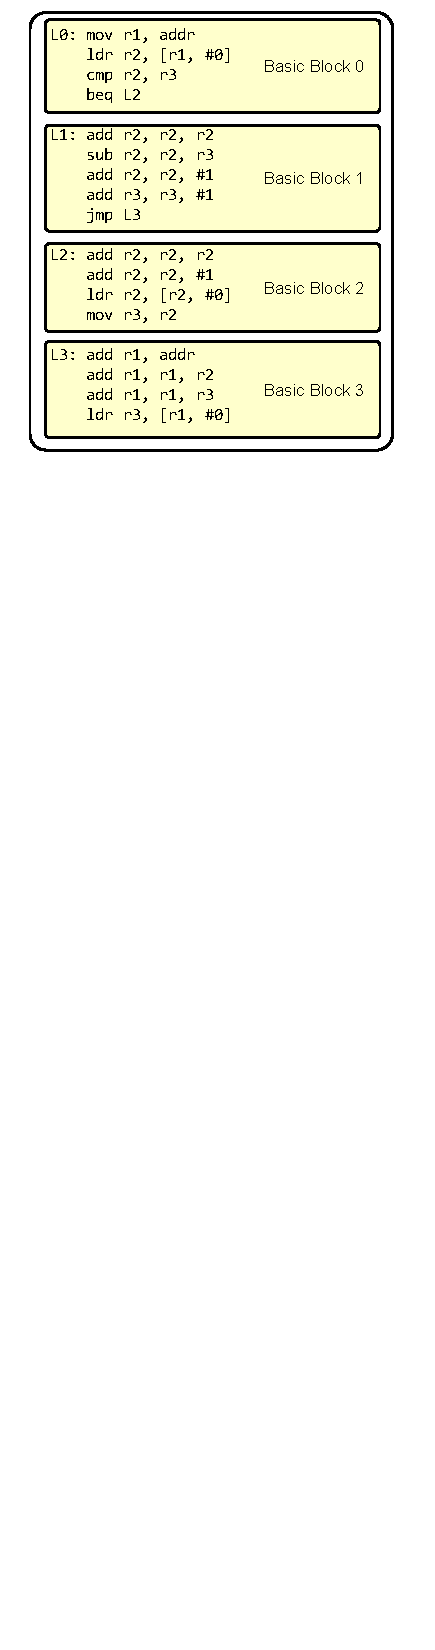
\includegraphics[]{monitoring_wcet/figs/code_example.pdf}
      \label{fig:monitoring_wcet.example.code_example} 
    }
    \end{subfigure}
    \hspace{-0.3in}
    \begin{subfigure}[Control flow graph.]{
      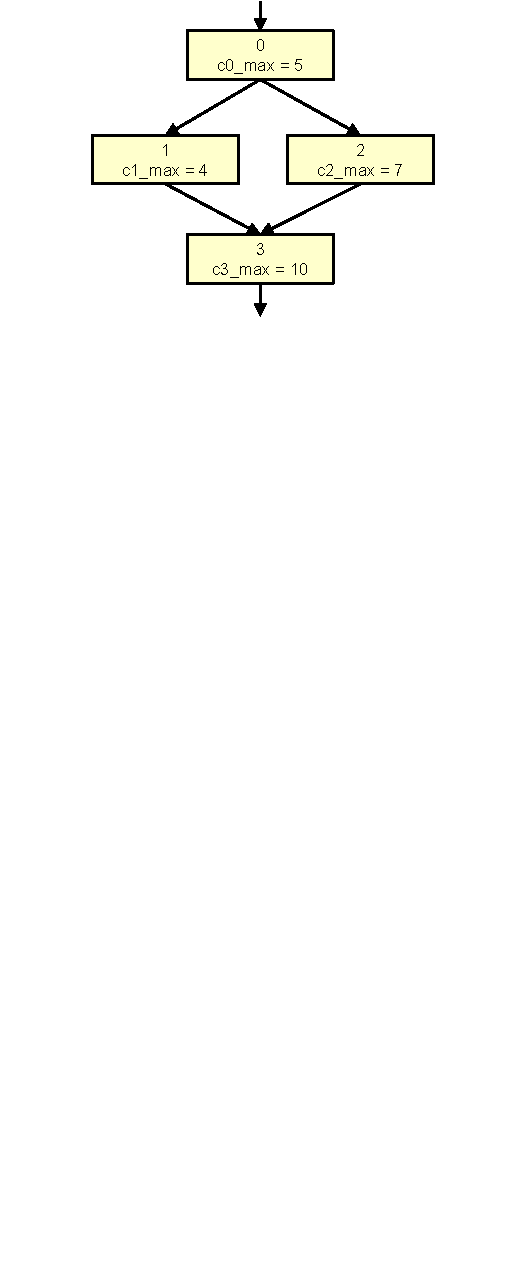
\includegraphics[]{monitoring_wcet/figs/cfg_example.pdf}
      \label{fig:monitoring_wcet.example.cfg_example} 
    }
    \end{subfigure}
    \hspace{-0.0in}
    \begin{subfigure}[Monitoring flow graph.]{
      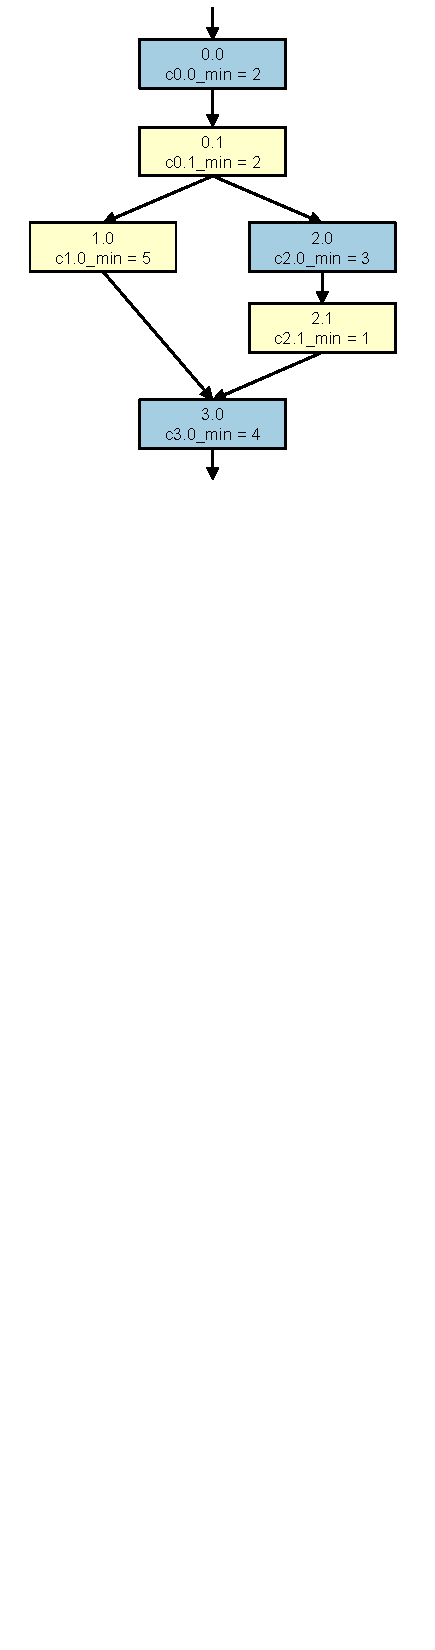
\includegraphics[]{monitoring_wcet/figs/mfg_example.pdf}
      \label{fig:monitoring_wcet.example.mfg_example} 
    }
    \end{subfigure}
  \end{center} 
  \caption{Code example with its corresponding control flow graph and
  monitoring flow graph. Blue (dark) nodes include a forwarded ({\tt ldr}) instruction.}
  \label{fig:monitoring_wcet.example.flow_graphs} 
  \vspace{-0.2in}
\end{figure}

An example code sequence is shown in
Figure~\ref{fig:monitoring_wcet.example.code_example}. Its associated control
flow graph is shown in
Figure~\ref{fig:monitoring_wcet.example.cfg_example}. We assume that the worst-case
execution time for each node has already been calculated using previous
methods. These execution times are labeled as {\tt cB\_max} in the figure.

In this example, let us assume that the monitoring technique requires loads and
stores to be forwarded, as in the case of an uninitialized memory check (UMC).
The monitoring task requires 5 cycles to handle a load and 7 cycles to handle a
store. Thus, the maximum execution time of the monitoring task, $t_{M, max}$,
is 7 cycles.

Because of the simplicity of the example, we assume that the FIFO only holds
one entry ($n_F = 1$). Thus, $l_{max} = n_F \cdot t_{M, max} = 7$.

\subsection{Creating the MFG}

The first step is to create the monitoring flow graph. For each node in the
CFG, the code represented by that node is analyzed. After any forwarded
instruction, in this case any load or store instructions, an edge is created,
dividing a node into two nodes in the monitoring flow graph. 
For example, the second instruction of node 0 in the CFG is a load instruction.
Thus, node 0 is split into two nodes in the MFG. The first node represents the
first two instructions and the second node represents the last two instruction. 

The resulting MFG is shown in Figure~\ref{fig:monitoring_wcet.example.mfg_example}.
Nodes that are blue (dark) include a forwarded instruction, which is located at
the end of the node. Nodes that are yellow (light) do not include a forwarded
instruction. The nodes in the graph are labeled with minimum ({\tt cB\_min})
rather than maximum execution times. It can be seen that node 2 from the CFG
corresponds to nodes 2.0 and 2.1 in the MFG. In this example, nodes in the CFG
were only transformed into at most two nodes in the MFG.  However, in general,
a CFG node will be transformed into a number of nodes in the MFG equal to the
number of forwarded instructions plus one.

\subsection{Calculating the Monitoring Load}
Once the MFG is constructed, a set of MILP constraints is generated for each
node. This process can be automated, but for this example we will construct the
constraints for one node by hand. Specifically we will consider node 3.0 in the
MFG. We will also calculate, by hand, the MILP solution for the node using some
assumed values for variables associated with other nodes. Note that all
variables are assumed to be non-negative unless otherwise specified.

{\bf Calculating input monitoring load:}
First, we will determine the worst-case input monitoring load for node 3.0,
$li_{3.0}$.  One set of constraints lower bounds the monitoring load by all
possible incoming monitoring loads.
\begin{align*}
  li_{3.0} \geq& lo_{1.0} \\
  li_{3.0} \geq& lo_{2.1} 
\end{align*}
Then, a set of constraints upper bounds this input monitoring load.
\begin{align*}
  li_{3.0} - 1000 \delta_{1.0} \leq& lo_{1.0} \\
  li_{3.0} - 1000 \delta_{2.1} \leq& lo_{2.1} \\
  \delta_{1.0} + \delta_{2.1} =& 1
\end{align*}
Here, the value 1000 is chosen arbitrarily but is known to be greater than
$|lo_{1.0} - lo_{2.1}|$.  A different value could have been chosen as long as
this condition was true.  $\delta_{1.0}$ and $\delta_{2.1}$ are binary
variables which can only assume values of $0$ or $1$.  To see how these
constraints work, suppose that $li_{1.0} = 4$ and $li_{2.1} = 7$. The
constraints are then evaluated as
\begin{align*}
  li_{3.0} \geq& 4 \\
  li_{3.0} \geq& 7 \\
  li_{3.0} - 1000 \delta_{1.0} \leq& 4 \\
  li_{3.0} - 1000 \delta_{2.1} \leq& 7 \\
  \delta_{1.0} + \delta_{2.1} =& 1
\end{align*}
The first pair of constraints ensures that $li_{3.0} \geq 7$. This means that
for the third constraint to hold, $\delta_{1.0} = 1$. If $\delta_{1.0} = 1$,
then by the last constraint, $\delta_{2.1} = 0$. Plugging this value into the
fourth constraint gives $li_{3.0} \leq 7$. Thus, the only possible solution is
$li_{3.0} = 7$ which is the maximum of $lo_{1.0}$ and $lo_{2.1}$.

{\bf Calculating output monitoring load:}
In order to determine the output monitoring load for node 3.0, we must first
calculate the change in monitoring node, $\Delta l_{3.0}$. Since there is a
forwarded instruction in node 3.0,
\begin{align*}
  \Delta l_{3.0} =& t_{M, max} - c_{3.0, min} \\
  =& 7 - 4 = 3
\end{align*}
We first create a variable, $lo'_{3.0}$ to represent the unbounded output
monitoring load.
\begin{align*}
  lo'_{3.0} =& li_{3.0} + \Delta l_{3.0}, \text{ } lo'_{3.0} \in (-\infty, \infty)
\end{align*}
Using the example input monitoring load previously calculated of $li_{3.0} =
7$, this unbounded output monitoring load is $lo'_{3.0} = 7 + 3 = 10$.  Then,
the following set of constraints determines the bounded output monitoring load,
$lo_{3.0}$.
\begin{subequations}
\begin{align}
  -1000\lambda_3 + 7\lambda_5 + 1000\lambda_6 =& 10 \label{eq:monitoring_wcet.lo1}\\ 
  \lambda_3 + \lambda_4 + \lambda_5 + \lambda_6 =& 1 \label{eq:monitoring_wcet.lo2}\\
  2 \delta_3 + \lambda_5 + \lambda_6 \leq& 2 \label{eq:monitoring_wcet.lo3}\\
  2 \delta_4 + \lambda_3 + \lambda_6 \leq& 2 \label{eq:monitoring_wcet.lo4}\\
  2 \delta_5 + \lambda_3 + \lambda_4 \leq& 2 \label{eq:monitoring_wcet.lo5}\\
  \delta_3 + \delta_4 + \delta_5 = 1 \label{eq:monitoring_wcet.lo6}\\
  7\lambda_5 + 7\lambda_6 =& lo_{3.0} \label{eq:monitoring_wcet.lo7}
\end{align}
\end{subequations}
The -1000 and 1000 values were chosen arbitrarily and only require that
$lo'_{3.0}$ to fall between them. $\delta_3$, $\delta_4$, and $\delta_5$ are
binary variables. By Constraint~\ref{eq:monitoring_wcet.lo2}, it can be seen
that all $\lambda_i$ are less than or equal to 1. Thus, in order for
Constraint~\ref{eq:monitoring_wcet.lo1} to hold, $\lambda_6 >  0$. Since
$\lambda_6 > 0$, Constraints~\ref{eq:monitoring_wcet.lo3} and
\ref{eq:monitoring_wcet.lo4} force $\delta_3$ and $\delta_4$ to both be zero.
From this, by Constraint~\ref{eq:monitoring_wcet.lo6}, $\delta_5 = 1$. Then, by
Constraint~\ref{eq:monitoring_wcet.lo5}, $\lambda_3$ and $\lambda_4$ are both
forced to be zero. If we now go back to the first two constraints, they are
reduced to
\begin{align*}
  7\lambda_5 + 1000\lambda_6 =& 10\\
  \lambda_5 + \lambda_6 =& 1 \\
\end{align*}
Solving this system of equations gives the solution $(\lambda_5, \lambda_6) =
(0.997, 0.003)$. Plugging these values into Constraint~\ref{eq:monitoring_wcet.lo7},
\begin{align*}
  lo_{3.0} =& 7\lambda_5 + 7\lambda_6 \\
  =& 7\cdot 0.997 + 7\cdot 0.003 \\
  =& 7
\end{align*}
Thus, the output monitoring load is indeed bound by the maximum monitoring load
of 7. Although this may seem to be a complicated series of calculations to
determine this obvious result, this set of constraints is required in order for
the piecewise linear, and thus non-linear, bounding function to be expressed in
an MILP problem.

{\bf Calculating the monitoring stall cycles:} The one remaining value that
needs to be determined for node 3.0 is the monitoring stall cycles. Based on
our previous calculations, the worst-case input monitoring load ($li_{3.0}$) is
7, the change in monitoring load ($\Delta l_{3.0}$) is 3, and the maximum
monitoring load ($l_{max}$) is 7. Thus, we expect the worst-case monitoring
stall cycles to be $(7+3)-7 = 3$. To handle this as an MILP problem, first the
unbounded monitoring stall cycles, $s'$, is calculated.
\begin{align*}
  s'_{3.0} =& li_{3.0} + \Delta l_{3.0} - l_{max}, \text{ } s'_{3.0} \in (-\infty, \infty) \\
  =& 7 + 3 - 7 = 3
\end{align*}
In this case, since $s'_{3.0}$ is positive, we expect $s_{3.0} = s'_{3.0}$. The
MILP problem determines $s_{3.0}$ using the following set of constraints.
\begin{subequations}
\begin{align}
  -1000\lambda_0 + 1000\lambda_2 =& 3 \label{eq:monitoring_wcet.s1}\\
  \lambda_0 + \lambda_1 + \lambda_2 =& 1 \label{eq:monitoring_wcet.s2}\\
  \delta_1 + \lambda_2 \leq& 1 \label{eq:monitoring_wcet.s3}\\
  \delta_2 + \lambda_0 \leq& 1 \label{eq:monitoring_wcet.s4}\\
  \delta_1 + \delta_2 =& 1 \label{eq:monitoring_wcet.s5}\\
  1000\lambda_2 =& s_{3.0} \label{eq:monitoring_wcet.s6}
\end{align}
\end{subequations}
The -1000 and 1000 values are chosen arbitrarily, only requiring that
$s'_{3.0}$ is between them. From Constraint~\ref{eq:monitoring_wcet.s1},
$\lambda_2$ must be positive. Since $\delta_i$ are binary variables,
Constraint~\ref{eq:monitoring_wcet.s3} then implies that $\delta_1 = 0$.
Constraints~\ref{eq:monitoring_wcet.s4} and \ref{eq:monitoring_wcet.s5} then
force $\delta_2 = 1$ and $\lambda_0 = 0$. The first two constraints then reduce
to
\begin{align*}
  1000\lambda_2 =& 3\\
  \lambda_1 + \lambda_2 =& 1 
\end{align*}
Solving this system of equations leads to $(\lambda_1, \lambda_2) = (0.997,
0.003)$ and thus calculating $s_{3.0}$ using
Constraint~\ref{eq:monitoring_wcet.s6}:
\begin{align*}
  s_{3.0} =& 1000 \lambda_2 \\
  =& 1000 \cdot 0.003 = 3
\end{align*}
This is the value for $s$ that we expected. If $s'$ had instead been negative,
then $\delta_1$ would be forced to 1 and $\lambda_2$ would be forced to 0. From
the last constraint, it can be seen that if $\lambda_2$ is 0, then $s$ is also
0.

\subsection{MILP Optimization}

In the previous subsection, the monitoring loads for one node were calculated
in detail. However, note that the output monitoring load for each node with an
edge pointing to node 3.0 was assumed to be a certain value. In an actual MILP
problem, these would be variables that are also being solved for. Solving for
these inter-related variables and determining the global maximum number of
cycles stalled due to monitoring is impractical to do by hand.  While the
amount of calculations may seem excessive for these simple examples, the
ability to formulate the problem in MILP is essential in order to solve large
problems. Given an MILP formulation, existing solvers \cite{lpsolve, cplex} can
be used to obtain the worst-case stall cycles.


\section{Evaluation}
\label{sec:monitoring_wcet.evaluation}

% Toolflow
\begin{figure}%[htb]
  \begin{center}
    \vspace{-0.1in}
    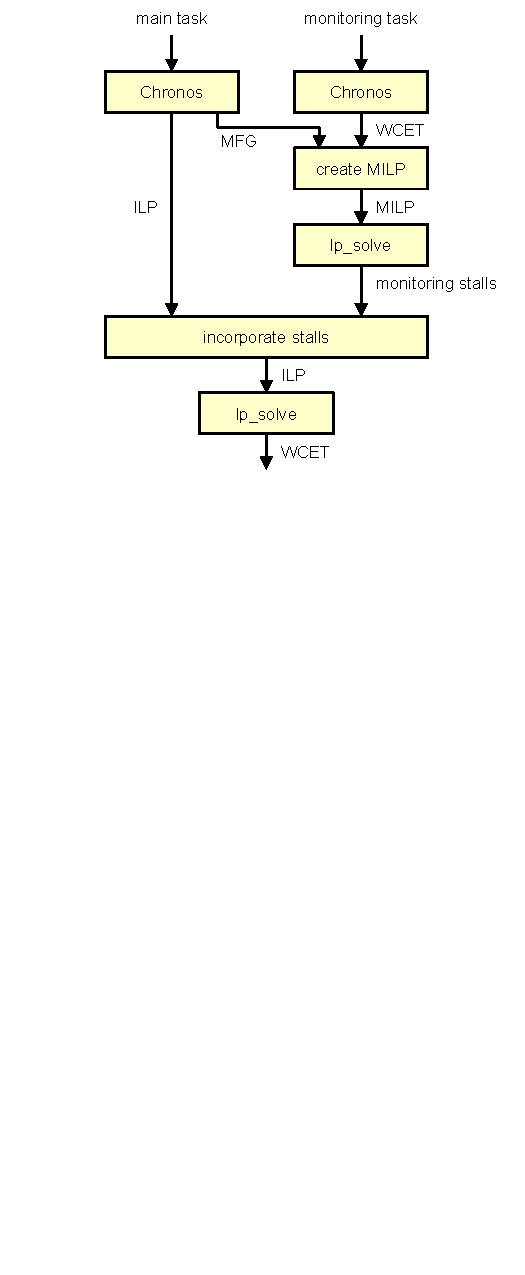
\includegraphics[height=2.2in]{monitoring_wcet/figs/toolflow.pdf}
    \vspace{-0.1in}
    \caption{Toolflow for WCET estimation of parallel monitoring.}
    \label{fig:evaluation.toolflow}
    \vspace{-0.3in}
  \end{center}
\end{figure}

% Results
\begin{table*}[htb]
  \begin{center}
    \begin{scriptsize}
    % WCET results 

\begin{tabular}{|l|l||r|r|r|r|r|r|r|}
\hline

\multirow{2}{*}{\bf Monitoring}&\multirow{2}{*}{\bf Experiment}&\multicolumn{7}{c|}{\bf Benchmark}       \\ \cline{3-9}
&&\multicolumn{1}{c|}{\tt cnt}&\multicolumn{1}{c|}{\tt expint}&\multicolumn{1}{c|}{\tt fdct}&\multicolumn{1}{c|}{\tt fibcall}&\multicolumn{1}{c|}{\tt insertsort}&\multicolumn{1}{c|}{\tt matmult}&\multicolumn{1}{c|}{\tt ns} \\ \hline \hline
\multirow{2}{*}{None}&wcet-none&64531&3483&1805&245&598&133668&5951 \\ \cline{2-9}
&sim-none&62931&2293&1805&245&598&133668&5951 \\ \hline \hline
\multirow{3}{*}{UMC}&sequential-umc&103052&3591&4382&257&2489&357453&10338 \\ \cline{2-9}
&wcet-umc&64550&3498&3035&245&2083&256120&5953 \\ \cline{2-9}
&sim-umc&62931&2297&2564&245&1864&235120&5951 \\ \hline \hline
\multirow{3}{*}{CFP}&sequential-cfp&151732&11669&1976&794&1174&231507&18623 \\ \cline{2-9}
&wcet-cfp&93544&8984&1805&547&677&133668&13614 \\ \cline{2-9}
&sim-cfp&72540&5247&1805&382&598&133668&9824 \\ \hline

\end{tabular}

    \end{scriptsize}
    \vspace{-0.1in}
    \caption{Estimated and observed WCET (clock cycles) with and without monitoring.}
    \label{tab:evaluation.wcet}
    \vspace{-0.2in}
  \end{center}
\end{table*}

% Calculated ratios
\begin{table*}[htb]
  \begin{center}
    \begin{tiny}
    % WCET results 

\begin{tabular}{|lll||r|r|r|r|r|r|r||r|r|r|}
\hline

\multicolumn{3}{|c||}{\multirow{2}{*}{\bf Ratio}}  &\multicolumn{7}{c||}{\bf Benchmark}      &\multicolumn{1}{c|}{\multirow{2}{*}{\bf min}}&\multicolumn{1}{c|}{\multirow{2}{*}{\bf max}}&\multicolumn{1}{c|}{\multirow{2}{*}{\bf geomean}} \\ \cline{4-10}
&&&\multicolumn{1}{c|}{\tt cnt}&\multicolumn{1}{c|}{\tt expint}&\multicolumn{1}{c|}{\tt fdct}&\multicolumn{1}{c|}{\tt fibcall}&\multicolumn{1}{c|}{\tt insertsort}&\multicolumn{1}{c|}{\tt matmult}&\multicolumn{1}{c||}{\tt ns}&&& \\ \hline \hline
wcet-none&:&sim-none&1.03&1.52&1.00&1.00&1.00&1.00&1.00&1.00&1.52&1.07 \\ \hline
wcet-umc&:&sim-umc&1.03&1.52&1.18&1.00&1.12&1.09&1.00&1.00&1.52&1.12 \\ \hline
wcet-cfp&:&sim-cfp&1.29&1.71&1.00&1.43&1.13&1.00&1.39&1.00&1.71&1.26 \\ \hline \hline
sequential-umc&:&wcet-umc&1.60&1.03&1.44&1.05&1.19&1.40&1.74&1.03&1.74&1.33 \\ \hline
sequential-cfp&:&wcet-cfp&1.62&1.30&1.09&1.45&1.73&1.73&1.37&1.09&1.73&1.45 \\ \hline \hline
wcet-umc&:&wcet-none&1.00&1.00&1.68&1.00&3.48&1.92&1.00&1.00&3.48&1.41 \\ \hline
wcet-cfp&:&wcet-none&1.45&2.58&1.00&2.23&1.13&1.00&2.29&1.00&2.58&1.55 \\ \hline

\end{tabular}

    \end{tiny}
    \vspace{-0.1in}
    \caption{Ratios comparing results from different experiments.} \label{tab:evaluation.ratios}
    \vspace{-0.3in}
  \end{center}
\end{table*}

\vspace{-0.0in}
\subsection{Experimental Setup}

Our toolflow for the proposed WCET method is shown in Figure~\ref{fig:evaluation.toolflow}. We
first use Chronos \cite{chronos-tool}, an open source WCET tool, to estimate
the WCET for the main task and the monitoring tasks. We also modified Chronos
to produce a MFG of the main task. This MFG and the monitoring task WCET are used to produce an MILP formulation as in
Section \ref{sec:formulation}. This MILP problem is solved
using lp\_solve \cite{lpsolve}, which produces the worst-case monitoring stall cycles for each forwarded
instruction. These monitoring stalls are combined into the ILP formulation that 
is originally generated for the main task to estimate the overall
WCET with parallel run-time monitoring. Although we use Chronos and lp\_solve
for our implementation, these components can be replaced with any WCET
estimation tool and LP solver respectively.

To evaluate the effectiveness of our WCET scheme, we compared its estimate
with a simple WCET bound from sequential monitoring (Section~\ref{sec:formulation:sequential})
as well as simulation results using the SimpleScalar tool \cite{simplescalar}.
In addition to the WCET estimates with monitoring, we also compared the results with
the WCET of the main task without monitoring, using both Chronos and simulations. 
% The baseline WCET allows us to study the overheads of parallel run-time monitoring
% in terms of the worst-case execution time.

%In order to examine
%how conservative the estimate was, we used the SimpleScalar simulator to
%simulate the benchmarks, both with and without monitoring. 

For the experiments, we configured Chronos and SimpleScalar to model simple processing cores
that execute one instruction per cycle for both main and monitoring cores and used an 8-entry FIFO.
This configuration represents typical embedded microcontrollers, and is designed to focus on 
the impact of parallel run-time monitoring by removing complex features such as branch prediction 
and caches.
%The experiments model an 8-entry FIFO that can buffer up to eight
%forwarded instructions. 
In the evaluation, we used seven benchmarks from the M\"alarden WCET benchmark suite \cite{malarden} 
and two monitoring techniques: uninitialized memory checks (UMC) and control flow protection (CFP).
UMC detects a software bug that reads memory without a write as briefly explained in 
Section~\ref{sec:arch}. CFP protects a program's control flow by checking a target address on
each control transfer \cite{arora-runtime05}. In this technique, a compiler determines a set of valid
targets for each branch and jump in the main task.
This information is stored on the monitoring core. 
On a branch or jump, the monitoring core ensures that the target is
contained in the list of valid targets.


\vspace{-0.05in}
\subsection{Results}

Table~\ref{tab:evaluation.wcet} shows the experimental results for each
benchmark under different configurations. The first set of rows show the WCET 
estimate from Chronos ({\tt wcet-none}) and actual run-times from simulations ({\tt sim-none}) without 
monitoring. The remaining rows show the WCET for the UMC and
CFP monitoring extensions. The results are shown for three different approaches:
a bound from sequential monitoring ({\tt sequential}), our approach ({\tt wcet}),
and simulations ({\tt sim}). The numbers indicate the number of clock cycles.
Appendix~\ref{sec:lptime} includes running times for these experiments.

Table~\ref{tab:evaluation.ratios} shows relative comparisons between
different configurations or WCET methods.
The first set of rows compare the WCET estimates from ILP or MILP formulations
with the worst-case simulation cycles for each monitoring setup. 
The results show that the analytical WCET estimates from our proposed scheme
are larger than the observed WCET by 0\% to 52\% for UMC and 0\% to 71\% for CFP, 
depending on the main task. This difference is comparable to the case without
parallel run-time monitoring, where the analytical WCET from Chronos
is larger than simulation results by 0\% to 52\%. 
In fact, for {\tt expint}, the majority of the difference is from the WCET
estimate of the main task rather than the effects of monitoring.
%In fact, for certain benchmarks, such as {\tt expint}, the majority of the difference 
%is due to estimating the
%WCET of the main task rather than the effects of monitoring. 
This result suggests that our WCET approach is not significantly more conservative than
the baseline WCET tool for the main task.

The second set of rows compare the bound from sequential monitoring and the WCET 
from our proposed method. 
For UMC, our approach shows up to a 74\% reduction in WCET estimates over the simple
bound. Similarly, for CFP, our method shows up to a 73\% improvement.
These results demonstrate that modeling the FIFO decoupling between the main and monitoring
tasks is important for obtaining tight WCET estimates of parallel
monitoring. 

Finally, the last two rows in Table~\ref{tab:evaluation.ratios} compare the WCET 
estimates with and without run-time monitoring.
The results show that the increase in WCET varies significantly depending on
benchmark and monitoring technique. Benchmarks with infrequent monitoring
events (forwarded instructions) show minimal overheads while ones with frequent
monitoring can see significant impacts.
Also, the benchmarks with large WCET increases differ between UMC and CFP.
Therefore, when applying parallel run-time monitoring techniques to real-time systems,
a careful WCET analysis for the given tasks and monitoring techniques 
needs to be performed. 

The impact of run-time monitoring on the execution time in our experiments
(up to 3.48x in UMC and 2.58x in CFP) is roughly in line with previous studies
on multi-cores without any hardware support \cite{chen08-lba, nagarajan08-dift}. 
The performance overheads will be much lower for multi-cores with optimizations 
\cite{chen08-lba} or heterogeneous monitors \cite{flexcore-micro10}. 
Our analysis technique does not depend on any specific monitoring core
microarchitecture and is applicable to more optimized architectures.

%Table~\ref{tab:evaluation.ratios} also compares the WCET estimated with each
%monitoring extension versus the WCET estimated without monitoring. For UMC, the
%WCET is increased by up to 3.48x and for CFP the WCET is increased up to 2.58x.
%However, for both extensions, there also exist benchmarks where the WCET is not
%increased. 

%%%%%%%%%%%%%%%%%%%%%%%%%%%%%%%%%%%%%%%%%%%%%%%%%%
% lp_solve time
%%%%%%%%%%%%%%%%%%%%%%%%%%%%%%%%%%%%%%%%%%%%%%%%%%

\subsection{Time to Solve Linear Programming Problem}
\label{sec:lptime}

% lp_solve time
\begin{table*}[htb]
  \begin{center}
    \begin{small}
    % lp_solve run time

\begin{tabular}{|l||r|r|r|r|r|r|r||r|r|r|}
\hline

\multirow{2}{*}{\bf Solver Target}&\multicolumn{7}{c||}{\bf Benchmark}      &\multicolumn{1}{c|}{\multirow{2}{*}{\bf min}}&\multicolumn{1}{c|}{\multirow{2}{*}{\bf max}}&\multicolumn{1}{c|}{\multirow{2}{*}{\bf geomean}} \\ \cline{2-8}
&\multicolumn{1}{c|}{\tt cnt}&\multicolumn{1}{c|}{\tt expint}&\multicolumn{1}{c|}{\tt fdct}&\multicolumn{1}{c|}{\tt fibcall}&\multicolumn{1}{c|}{\tt insertsort}&\multicolumn{1}{c|}{\tt matmult}&\multicolumn{1}{c||}{\tt ns}&&& \\ \hline \hline
stall-umc&17.789&6.256&21.733&0.043&0.39&161.796&3.655&0.043&161.796&4.224 \\ \hline
stall-cfp&3.691&97.93&0.038&0.024&0.025&14.209&1.474&0.024&97.930&0.778 \\ \hline \hline
sequential-umc&0.006&0.004&0.004&0.005&0.002&0.004&0.006&0.002&0.006&0.004 \\ \hline
sequential-cfp&0.007&0.001&0.003&0.002&0.003&0.006&0.003&0.001&0.007&0.003 \\ \hline \hline
wcet-none&0.003&0.003&0.004&0.002&0.002&0.002&0.001&0.001&0.004&0.002 \\ \hline
wcet-umc&0.004&0.004&0.003&0.001&0.004&0.005&0.002&0.001&0.005&0.003 \\ \hline
wcet-cfp&0.002&0.007&0.005&0.004&0.003&0.005&0.004&0.002&0.007&0.004 \\ \hline

\end{tabular}

    \end{small}
    \vspace{-0.1in}
    \caption{Running time of lp\_solve in seconds to determine worst-case stalls
    (stall), sequential bound (sequential), and worst-case execution times (wcet).}
    \label{tab:appendix.runtime}
    \vspace{-0.2in}
  \end{center}
\end{table*}

The most time intensive portion of the WCET analysis is the actual solving of
the linear programming (LP) problem. For our experiments, we used lp\_solve
5.5.2.0 \cite{lpsolve} as our LP solver. These experiments were run on a 2.67
GHz Xeon E5430 quad-core processor with 4 GB of RAM. The running times for
lp\_solve are shown in Table~\ref{tab:appendix.runtime}.  The first set of rows
show the running time for determining the worst-case stalls from the monitoring flow
graph ({\tt stall}). The second set of rows show the lp\_solve running time for
finding the sequential bounds. The final set of rows show the running time for
determining the overall WCET ({\tt wcet}). For {\tt wcet-umc} and {\tt
wcet-cfp}, this is for the ILP problem given the worst-case stalls .

The running times for the {\tt sequential} cases and the {\tt wcet} cases are very
similar. This is because these cases are all solving essentially the same
problem with different numbers. That is, for a given benchmark, these different
cases are all solving a linear programming problem for the same control flow
graph (CFG). As a result, the number of variables and the set of
constraints is the same, though the WCET for each basic block changes depending
on the extension and the estimation method. The {\tt stall} cases have a longer
running time.
This is due to the fact that a MFG has more nodes than its corresponding CFG.
The increased number of nodes also implies more variables and more constraints.





\chapter{Slack-Aware Opportunistic Monitoring for Real-Time Systems}
\label{chap:monitoring_hard_drop}

\section{Introduction}
\label{sec:monitoring_hard_drop.introduction}

% Run-time monitoring has high WCET.
In the last chapter, we showed how the WCET of run-time monitoring could be
estimated. By accounting for this WCET, this allows run-time monitoring to be
implemented in traditional real-time frameworks while giving strong guarantees
that deadlines will be met. However, the increase in WCET introduced by
run-time monitoring can be quite high, requiring a large amount of slack in a
system's schedule in order to support it. For example,
Section~\ref{sec:monitoring_hard_drop.evaluation} showed that even an
aggressive implementation of UMC showed increased WCET of 3.5x compared to
without monitoring. A more realistic implementation that includes deciding
which tasks to run in software can show increases of WCET of up to 12x compared
to the baseline.  Thus, applying monitoring to real-time systems requires a
large increase in the time allocated to tasks.  Currently, if a real-time
system cannot support this extra utilization, then monitoring cannot be applied
to the system.  

% Our solution is based on dynamic slack.
In this chapter, we describe a system that greatly decreases the amount of time
that must be statically allocated to tasks in the worst case (i.e., WCET) in
order to enable monitoring. Specifically, this system exploits dynamic slack in
order to opportunistically perform as much monitoring as possible within the
time constraints of the system. This is based on three key observations:
\begin{enumerate}
  \item Tasks often run faster than their worst-case time.
  \item The performance impact of monitoring is rarely equal to the worst-case impact.
  \item Performing partial monitoring can still provide some degree of protection.
\end{enumerate}
Since tasks typically run faster than their conservatively estimated WCET,
there exists dynamic slack at run-time that can be used for monitoring.
Similarly, the estimation of the WCET of monitoring is conservative. In
actuality, the overheads of monitoring are much lower, as shown by the
average-case performance impact. Finally, although performing all monitoring
operations in full is preferred, performing only a portion of the monitoring
still gives increased protection over a system with no monitoring applied.
By shifting the decision of whether to enable or disable monitoring to
run time, we are able to trade off monitoring coverage in order to reduce the
WCET impact of monitoring. The system we present decides whether or not to
perform monitoring based on whether there is enough dynamic slack to account
for the worst-case performance impact of the monitoring.

% Key issue is false positives
A main challenge in skipping monitoring operations is ensuring that the monitor
can still run in a useful manner. Although we trade off the coverage provided
by monitoring in order to meet timing requirements, we must also  guarantee
that no false positives occur in order to prevent false alarms.
We prevent false positives through the use of a dropping task that invalidates
metadata when monitoring is skipped.
With hardware optimizations, this invalidation can be handled with no impact on
the task's WCET. In addition, the hardware architecture we present skips
monitoring on invalidated metadata, saving dynamic slack to be used for useful
monitoring on valid metadata.

The rest of this chapter is organized as follows. In
Section~\ref{sec:monitoring_hard_drop.drop}, we discuss how to decide when to
skip monitoring and how to handle this in a safe manner. Hardware optimizations
for handling this dropping operation are presented in
Section~\ref{sec:monitoring_hard_drop.hwdrop}. We present our evaluation
methodology and experimental results in
Section~\ref{sec:monitoring_hard_drop.evaluation}. 


\section{Opportunistic Monitoring}
\label{sec:monitoring_hard_drop.drop}

In this section we present a framework for opportunistically performing
monitoring in such a way as to ensure that the main task's execution time does
not exceed its WCET bound. The basic idea is that on a monitoring event, the
system checks whether there is enough slack to account for the worst-case
impact of monitoring on the main task's execution time. If there is enough
slack, then the monitoring task proceeds. If there is not enough slack, then
instead the event is dropped. 

There are two main challenges in this scheme. The first is how to measure slack
at run time and decide when it is necessary to drop monitoring tasks, which we
discuss in Section~\ref{sec:monitoring_hard_drop.drop.slack}. Once it has been
decided to drop a monitoring event, the second issue is how to drop the
monitoring task in such a way as to maintain the correctness of the monitoring
scheme which we discuss in
Section~\ref{sec:monitoring_hard_drop.drop.dropping_tasks}.

\subsection{Measuring Slack}
\label{sec:monitoring_hard_drop.drop.slack}

% Shows execution time and slack
\begin{figure}
  \begin{center}
    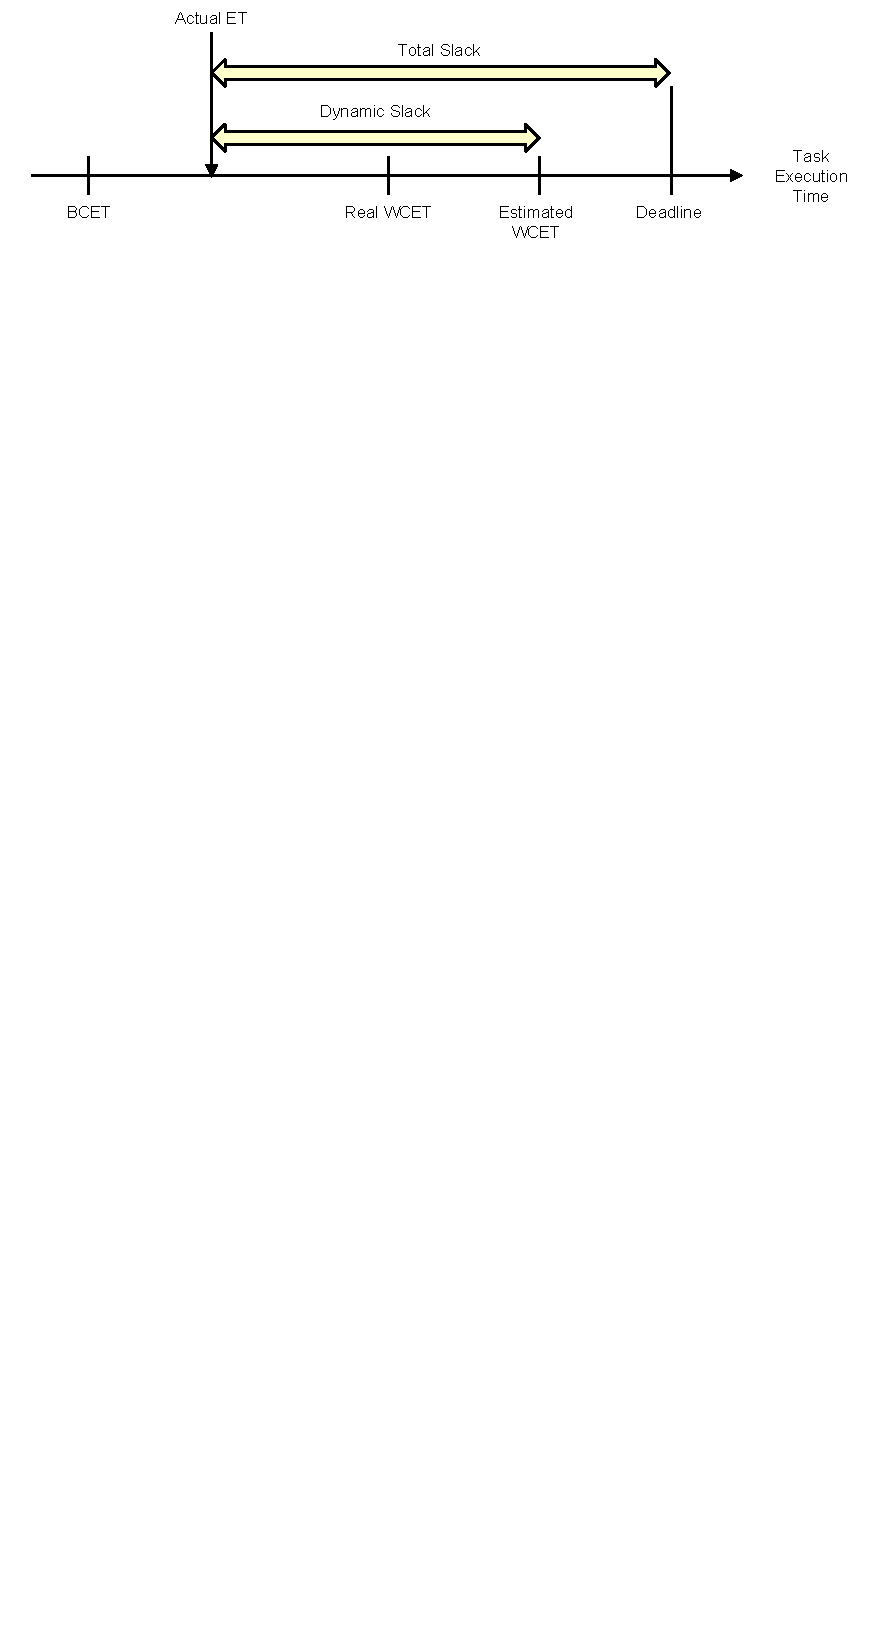
\includegraphics{monitoring_hard_drop/figs/slack_defn.pdf}
    \caption{Dynamic slack and total slack.}
    \label{fig:monitoring_hard_drop.drop.slack_defn} 
  \end{center}
\end{figure}

In order to decide when it is possible to perform monitoring, we must be able
to measure the dynamic slack available.  Dynamic slack is defined as the
difference between a task's expected worst-case execution time (WCET) and its
actual execution time \cite{multi_task_visa-rtss04}. This is only a
portion of the total slack which is the difference between a task's finish time
and its deadline (see Figure~\ref{fig:monitoring_hard_drop.drop.slack_defn}).
Although the dynamic slack only accounts for a portion of the total slack, we
only focus on dynamic slack because this is the portion of slack that is
specific to a task.  Additional slack in the schedule could be assigned to a
specific task to be used for monitoring by the system designer or scheduler.
For brevity, we will use the term slack to refer to dynamic slack.

% Diagram showing sub-tasks and slack accumulation/usage
\begin{figure}
  \begin{center}
    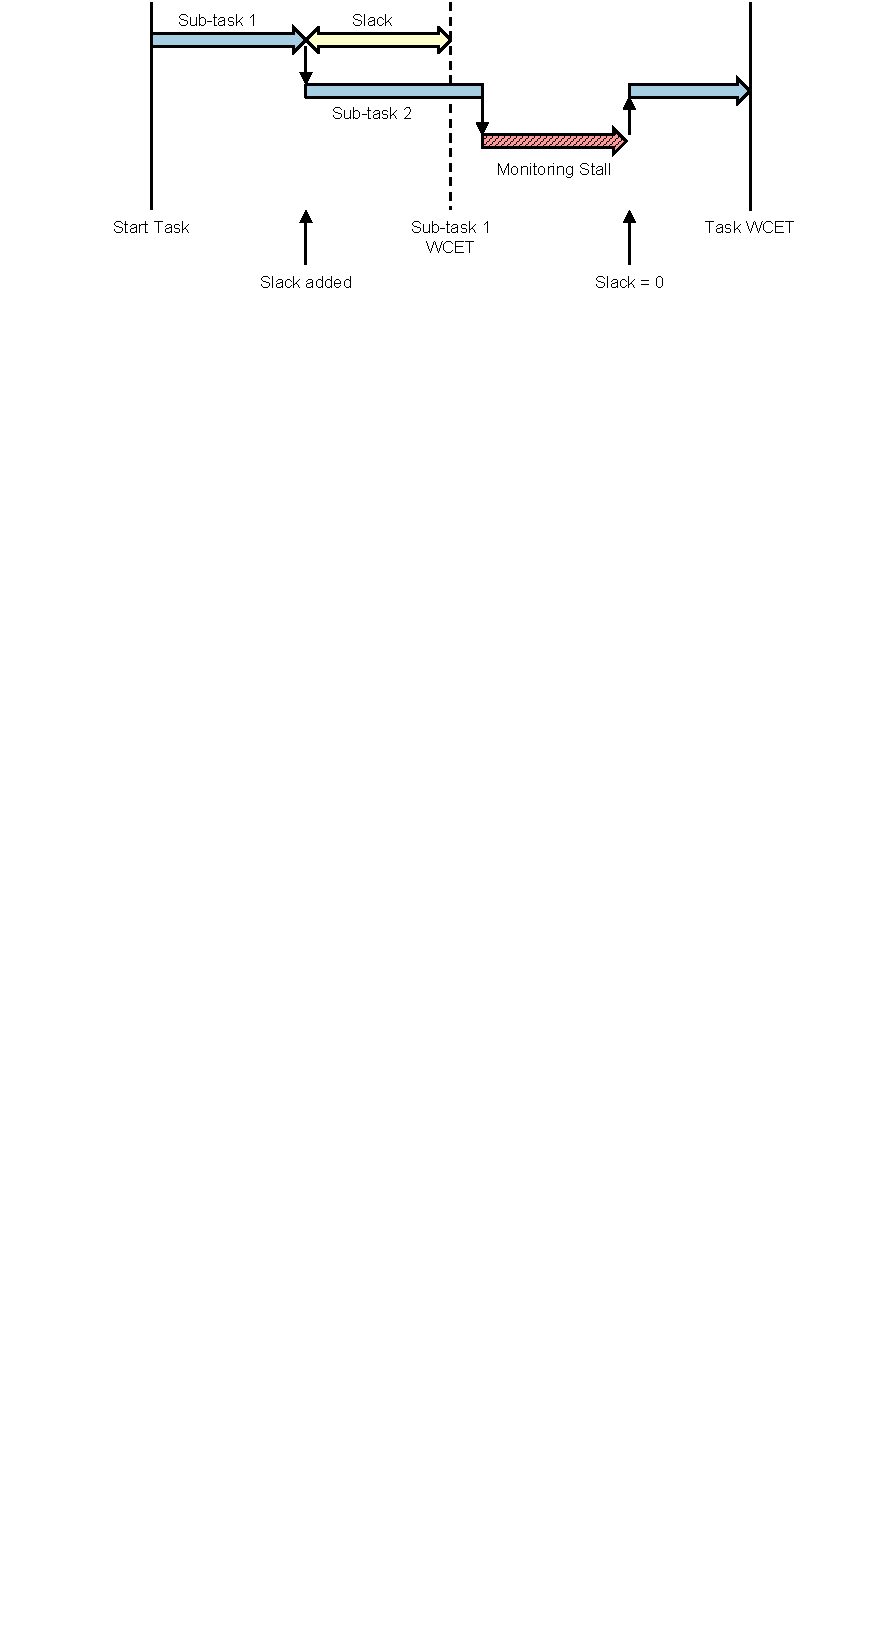
\includegraphics{monitoring_hard_drop/figs/task_slack.pdf}
    \caption{Dynamic slack increases when a sub-task finishes early. Slack is
    consumed as monitoring causes the task to stall.}
    \label{fig:monitoring_hard_drop.drop.task_slack} 
  \end{center}
\end{figure}

In order to perform monitoring as the task runs, we need to be able to measure
dynamic slack as the task runs.  We can track dynamic slack by setting a number
of checkpoints throughout the task.  These checkpoints effectively divide the
task into a number of sub-tasks.  For each of these sub-tasks, the sub-task's
WCET is determined.  At run-time when a sub-task finishes, the difference
between its actual run-time and its WCET is the slack generated by the
sub-task.  Specifically, we insert code to mark each sub-task boundary.  At the
beginning of a sub-task, the WCET of a sub-task is loaded into a timer. Each
cycle, the timer decreases. At the end of a sub-task, the remaining value in
the timer is the slack generated by the sub-task. This value is added to the
current slack.  An example of this process is shown in
Figure~\ref{fig:monitoring_hard_drop.drop.task_slack}. In our experiments, the
division of a task into sub-tasks was done by hand but this process could be
automated to divide a task using function boundaries, code length, or some
other criteria.  In addition to the slack accumulated while running, a portion
of \emph{headstart slack} can be initially assigned by the designer or
scheduler to the task. For example, if the designer knows that static slack
exists in the schedule, this slack can be added to the initial dynamic slack of
a task to be used for monitoring.

By accumulating this slack as the task runs, we can determine whether
monitoring can be performed while still meeting the real-time constraints. If
the worst-case impact of a monitoring task on the main task is less than the
accrued slack, then the monitoring task can execute.  If running the monitoring
task causes the main task to stall, then slack is consumed.
Slack was initially generated since the main task was running ahead of its
WCET, so stalling up to the slack time will not cause the main task to exceed
its WCET (see Figure~\ref{fig:monitoring_hard_drop.drop.task_slack}). In the
best case, the monitoring task executes entirely in parallel and does not
affect the main task and thus consumes no slack. On the other hand, if the
worst-case impact of the monitoring task on the main task's execution time is
greater than the slack, then, conservatively, the monitoring task cannot be
run. Instead, it must be dropped in order to guarantee that the main task
finishes within its WCET.

\subsection{Dropping Tasks}
\label{sec:monitoring_hard_drop.drop.dropping_tasks}

Dropping a monitoring task implies that some functionality of the monitor has
been lost.  This may cause either false negatives, where an error that occurs
in the main task's execution is not detected, or false positives, where the
monitor incorrectly believes an error has occurred.  For example, a false
positive can occur for UMC if a store monitoring event is dropped. This causes
the memory location of the store to not be marked as initialized. A subsequent
load for the memory location will incorrectly cause an error to be raised.  We
accept false negatives as the loss in coverage that we trade off in order to
ensure the WCET of the main task is met. However, we must safely drop
monitoring events in such a way as to avoid false positives so that the system
does not incorrectly raise an error.

% Need for a dropping task to prevent false positives.
In order to ensure that no false positives occur, we need to run a
\emph{dropping task} when a monitoring task is dropped.  The specifics of how
this dropping task operates may vary for different monitoring schemes. However,
in analyzing various monitoring schemes, we found that most monitoring tasks
perform operations of primarily two types: \emph{checks} and \emph{metadata
updates}. Monitoring tasks \emph{check} certain properties to ensure correct
main task execution and they \emph{update} metadata for bookkeeping. Skipping a
check operation can only cause false negatives and will never cause a false
positive. Therefore, the dropping task may simply skip a check operation.
Skipping an update operation can cause false negatives but may also cause false
positives.  Essentially, when an update operation is skipped, we can no longer
trust the corresponding metadata. In some cases, the dropping task can handle
this by setting the metadata to a neutral value that will not cause false
positives (e.g., cleared or null). A more general solution is for the dropping
task to mark the corresponding metadata as invalid, to prevent future false
positives.

% WCET for SW vs. HW vs. neither scheme
\begin{figure}
  \begin{center}
    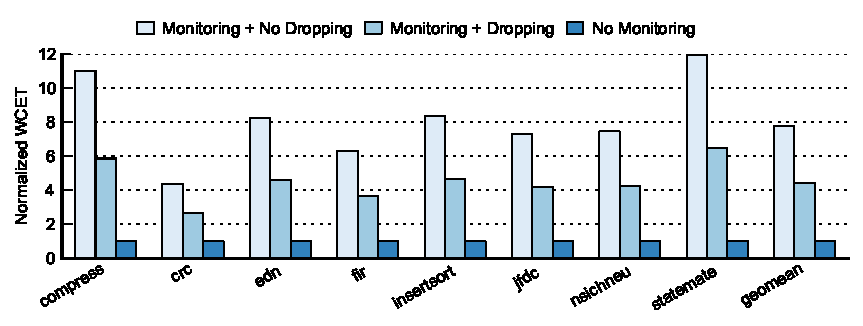
\includegraphics{monitoring_hard_drop/data/sw_drop_wcet.pdf}
    \caption{WCET with original monitoring task, with software dropping task,
    and with no monitoring for UMC. Results are normalized to the WCET with no
    monitoring.}
    \label{fig:monitoring_hard_drop.drop.sw_drop_wcet} 
  \end{center}
\end{figure}

% Want to minimize WCET of dropping task
In the worst case, no monitoring can be done and the system must ensure that
there is enough time to run a dropping task for every monitoring event in order
to avoid false positives.  Thus, the main task's WCET estimation must be
modified to take into account the worst-case impact due to the dropping task.
By minimizing the dropping task's execution time, the impact on the main task's
WCET can be much lower than the impact due to the monitoring task.
Figure~\ref{fig:monitoring_hard_drop.drop.sw_drop_wcet} compares the original WCETs
with and without monitoring to the WCET with dropping tasks implemented in
software for UMC. The WCETs are normalized to the WCET without monitoring.  The
WCET with dropping is reduced by 43\% on average from the WCET without
dropping. 


\section{Hardware-Based Dropping Architecture}
\label{sec:monitoring_hard_drop.hwdrop}

In Section~\ref{sec:monitoring_hard_drop.drop}, we presented a general
framework for how to design a system that allows dropping of monitoring tasks
to ensure the main task's execution time. However, implementing this framework
in software still has significant impacts on the WCET as shown in
Figure~\ref{fig:monitoring_hard_drop.drop.sw_drop_wcet}.  In this section, we
present a novel hardware architecture that eliminates these impacts to the main
task's WCET.

There are two main sources that affect the main task's WCET: the additional
code for keeping track of slack and the impact of the dropping task.  In
Section~\ref{sec:monitoring_hard_drop.hwdrop.slack}, we describe hardware to
keep track of slack and to make the decision on whether to run the monitoring
or dropping task.  In Section~\ref{sec:monitoring_hard_drop.hwdrop.drop}, we
present a hardware-based metadata invalidation scheme that allows dropping to
be performed in a single cycle.  By handling the dropping in a single cycle,
the throughput is able to match the throughput of the main core.
Section~\ref{sec:monitoring_hard_drop.hwdrop.filter} builds upon the
hardware-based invalidation scheme to filter out monitoring tasks for invalid
metadata in order to reserve slack for more useful cases of running the
monitoring task. Finally, in
Section~\ref{sec:monitoring_hard_drop.hwdrop.full_arch} we show the full
architecture.

\subsection{Slack Tracking}
\label{sec:monitoring_hard_drop.hwdrop.slack}

% Slack tracking hardware
\begin{figure}
  \begin{center}
    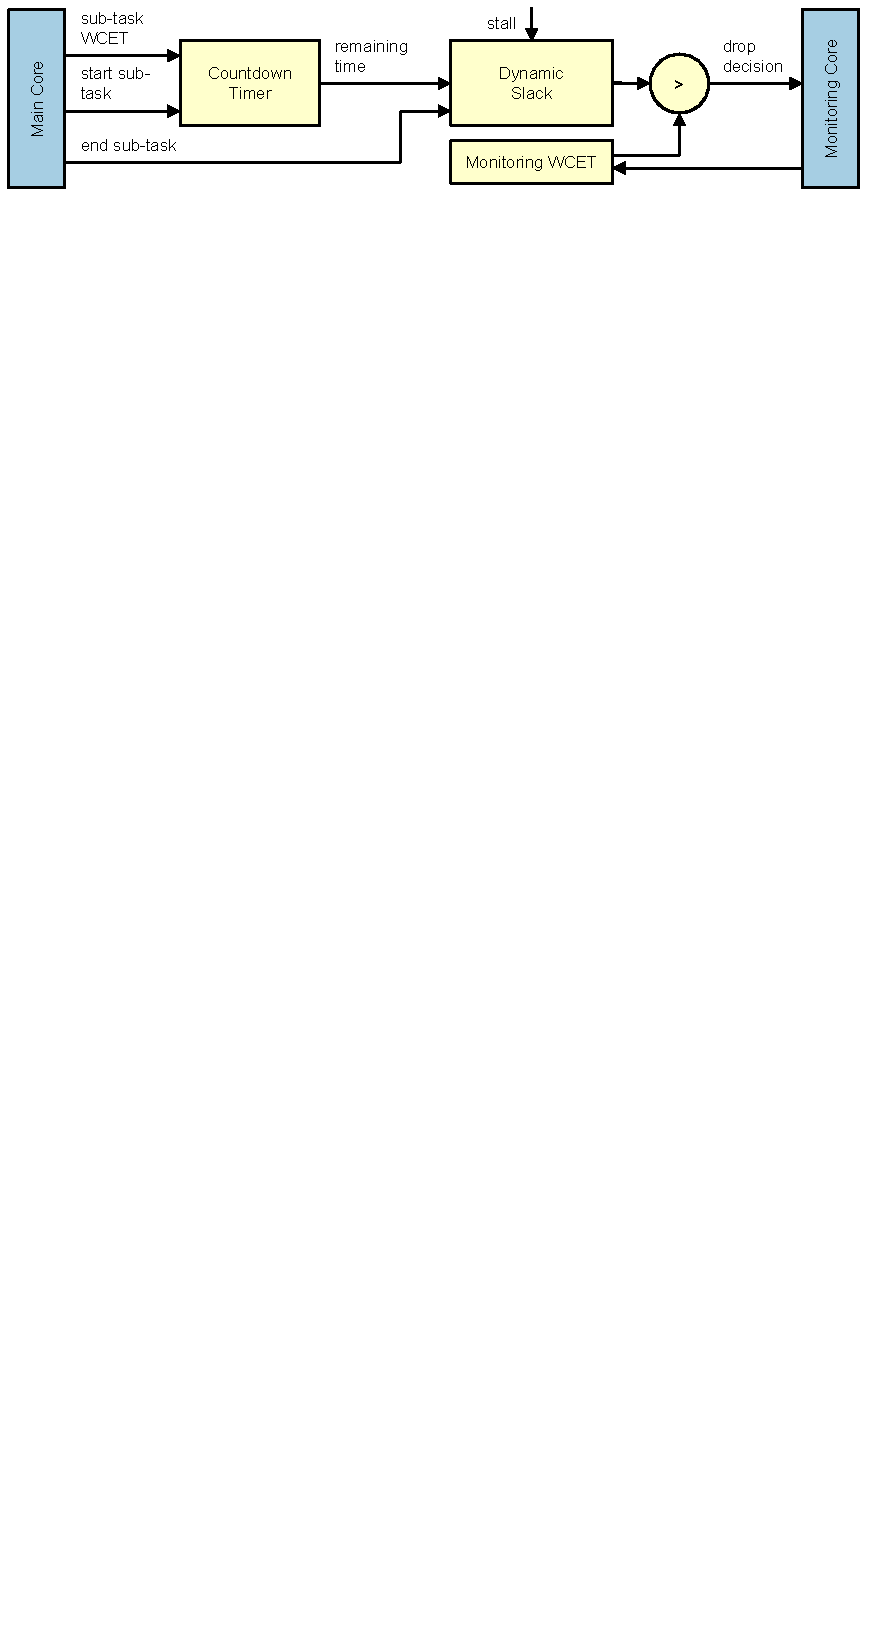
\includegraphics{monitoring_hard_drop/figs/slack_tracking.pdf}
    \caption{Hardware modules for keeping track of slack and making a drop decision.}
    \label{fig:monitoring_hard_drop.hwdrop.slack_tracking} 
  \end{center}
\end{figure}

Figure~\ref{fig:monitoring_hard_drop.hwdrop.slack_tracking} shows a hardware slack tracking module
(STM). In order to keep track of slack, a countdown timer is loaded with a
sub-task's WCET at the start of a sub-task and counts down each cycle. At the
end of a sub-task, the remaining time in this countdown timer is added to the
current dynamic slack which is stored in a register. At the start of a task,
the dynamic slack register is cleared and set to the headstart slack if one is
specified.  In addition, whenever the main task is stalled due to the
monitoring core, this dynamic slack is decremented.

The currently measured dynamic slack is used to determine whether the
monitoring task can run in full. When the monitor is initialized, the monitor
will load its worst-case needed slack in order to perform the monitoring task
into a register. When there is a monitoring event in the FIFO to be processed,
a hardware comparator checks whether the dynamic slack is greater than or equal
to the necessary slack for full monitoring. If enough slack exists, the
monitoring core is signaled to perform the monitoring task. Otherwise, the
monitoring event is dropped.

\subsection{Metadata Invalidation Module}
\label{sec:monitoring_hard_drop.hwdrop.drop}

% Metadata invalidation module
\begin{figure}
  \begin{center}
    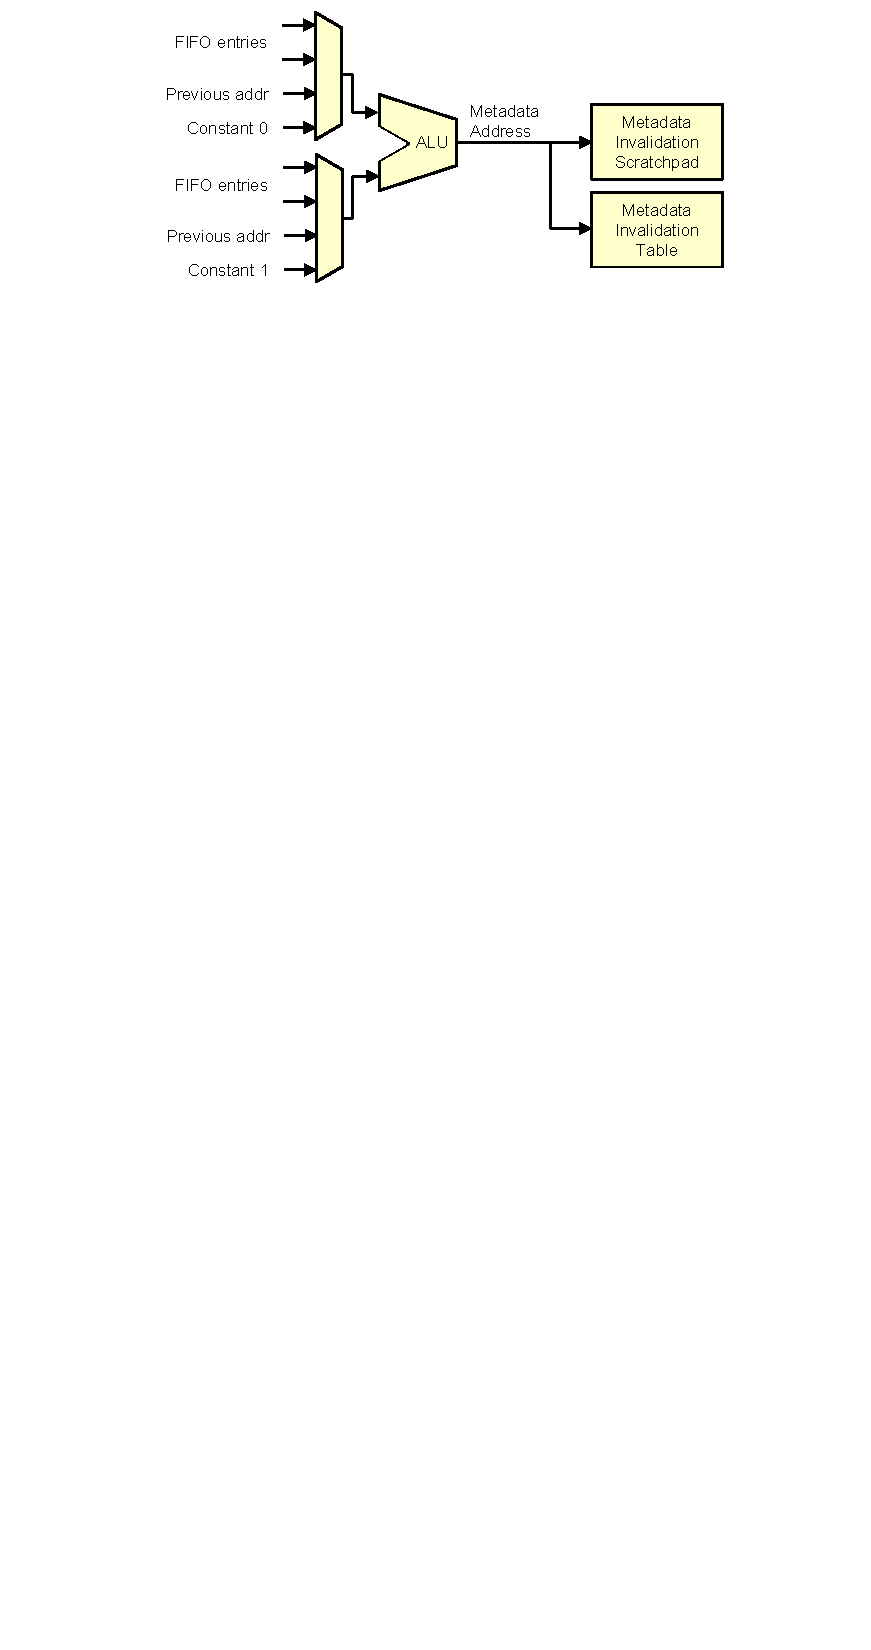
\includegraphics{monitoring_hard_drop/figs/mim.pdf}
    \caption{Metadata invalidation module (MIM).}
    \label{fig:monitoring_hard_drop.hwdrop.mim}
  \end{center}
\end{figure}

In the worst-case, all monitoring events must be dropped. Thus, it is important
that whatever dropping task needs to be run has a minimal impact on the main
task. If this dropping task can match the maximum throughput of the main core,
then the original WCET of the main task is not affected, removing the need to
redo the WCET analysis. In this section, we present a hardware architecture
that can handle dropping monitoring events in a single cycle, matching the
throughput of the main core.

As mentioned in Section~\ref{sec:monitoring_hard_drop.drop.dropping_tasks}, the dropping task must
invalidate metadata on a dropped monitoring event.  Thus, we have designed a
hardware module to perform this invalidation. Figure~\ref{fig:monitoring_hard_drop.hwdrop.mim} shows
a block diagram of this module, which we call the metadata invalidation module
(MIM).  When the slack tracking module indicates that a monitoring task must be
dropped, the metadata invalidation module sets a bit in the metadata
invalidation table (MIT) corresponding to the metadata to be invalidated.  The
metadata to be invalidated depends on the monitoring scheme and the monitoring
event. For example, for the uninitialized memory check monitoring scheme, on a
store event, metadata corresponding to the memory access address is set to
indicate initialized memory. Thus, on a dropped event, the MIM must be able to
calculate the address of this metadata in order to set a corresponding
invalidation flag.  The MIM includes a small ALU to perform these simple
address calculations. Since this metadata address mapping varies for different
monitoring schemes, the inputs to the ALU can either be data from the
monitoring event, the previous metadata address, or a constant. The input
selection and the ALU operation to perform are looked up from a configuration
table depending on the type of monitoring event.  The monitor sets up this
configuration table during initialization.

In order for this dropping operation to match the throughput of the main core
(i.e., up to one monitoring event per cycle), the metadata invalidation
information is stored on-chip. The MIT is implemented as a small on-chip
memory, similar to a cache. This memory stores invalidation flags and is
indexed using part of the metadata address. It stores the remaining portion of
the address as a tag. Unlike a cache, if an access misses in the MIT, there is
no lower-level memory structure to go to. This is done in order to ensure that
the MIM can handle a monitoring event every cycle. Instead of backing the MIT
with lower-level memory, if writing to the MIT would force an eviction, we
instead mark the corresponding cache set as ``aliased''. From this point on, we
are forced to conservatively consider any metadata that would be mapped to this
cache set as invalid, regardless of the tag corresponding to its metadata
invalidation address. This reduces the amount of useful monitoring that can be
done, but guarantees that the dropping hardware can match the main core's
throughput. These aliased sets can be reset by re-initializing (e.g., resetting
to a null value) all metadata that could map to the aliased set. By using
dynamic slack or a dedicated periodic task, the system can occasionally reset
aliased sets. In either case, a sufficiently sized MIT should ensure that
aliasing is rare.

In some cases we would like to use the MIM hardware to operate in such a way as
to ensure that aliasing does not occur. For example, we found that some
monitoring schemes save metadata information about registers. Since this
metadata is used often, it is important to manage it in such a way that
aliasing does not occur. Thus, the MIM also includes a metadata invalidation
scratchpad (MISP). This MISP is explicitly addressed and it is up to the system
designer to utilize it in such a way that aliasing will not occur.

Both the MIT and MISP are accessible by the monitor. This allows the monitor to
be aware of what has been invalidated. The monitor can also re-validate
metadata when possible, such as when the monitoring task writes metadata
values.

We note that the MIM was designed with the idea of marking certain metadata as
valid or invalid with a 1-bit flag. However, in general the MIM simply sets or
clears a bit based on a calculated address. We expect that for certain
monitoring schemes, designers may be able to use the MIM in new ways such as
using the MIT and MISP to directly express certain metadata.
Section~\ref{sec:monitoring_hard_drop.extensions} shows how the MISP can be
used to directly express the register file taint metadata used for a dynamic
information flow tracking (DIFT) scheme.

\subsection{Filtering Invalid Metadata}
\label{sec:monitoring_hard_drop.hwdrop.filter}

% Metadata filtering module
\begin{figure}
  \begin{center}
    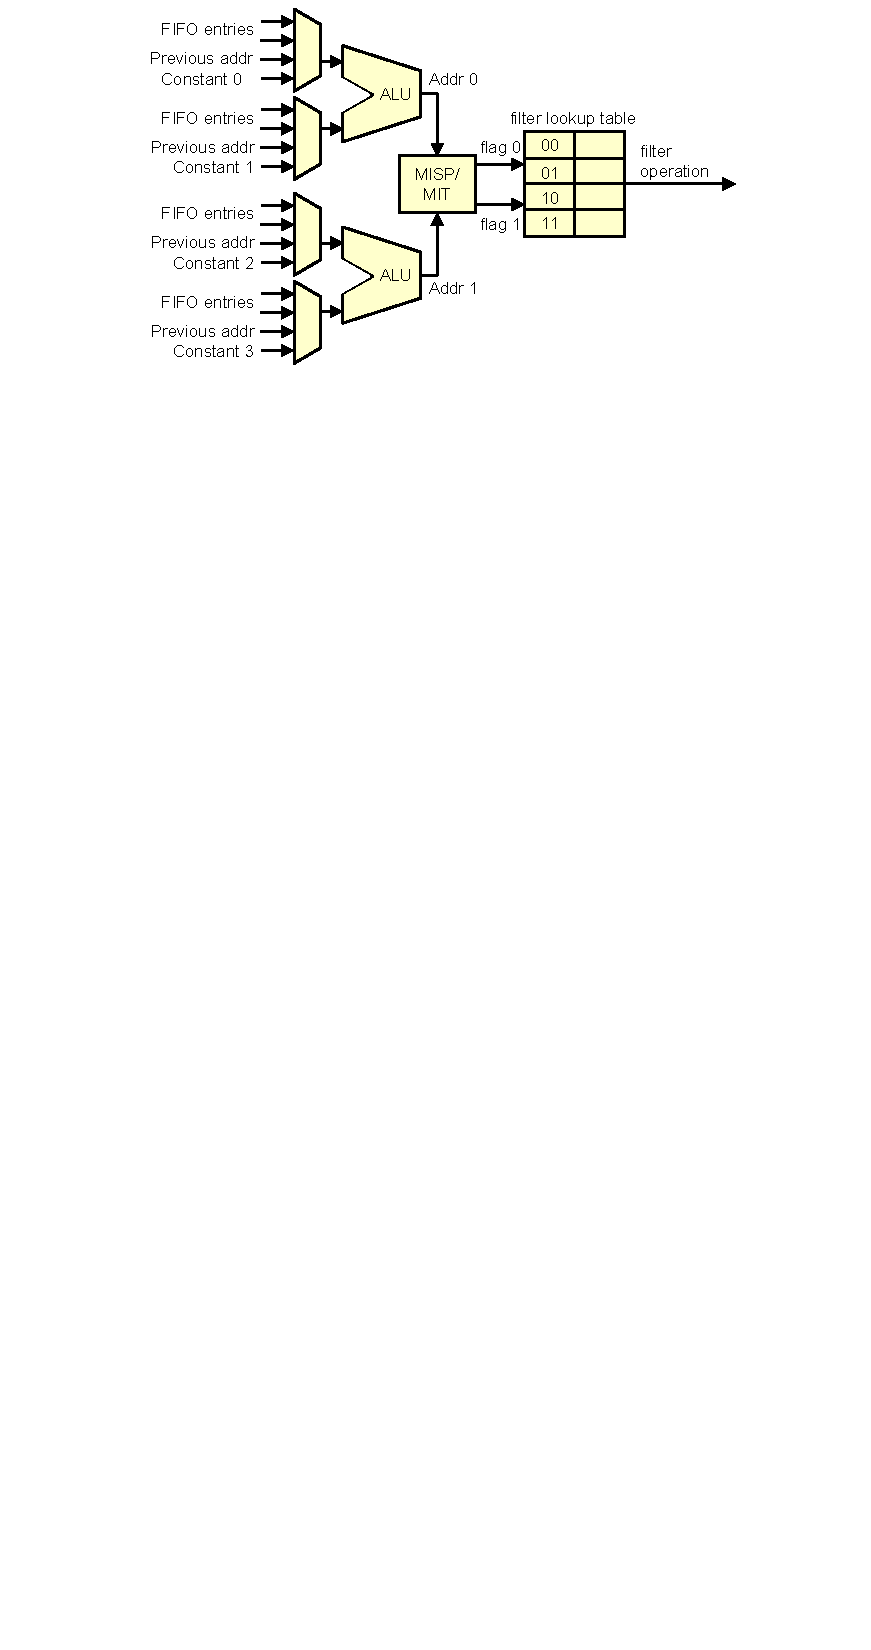
\includegraphics{monitoring_hard_drop/figs/mfm.pdf}
    \caption{Metadata filtering module (MFM).}
    \label{fig:monitoring_hard_drop.hwdrop.mfm}
  \end{center}
\end{figure}

Given that certain metadata becomes invalidated by the metadata invalidation
module, performing check and update monitoring operations based on the invalid
metadata is not useful. Thus, we can drop these monitoring tasks. By skipping
these invalid monitoring tasks, slack can be reserved for monitoring tasks
which operate on valid metadata. Determining when a monitoring event can be
filtered out in this manner is done by the metadata filtering module (MFM)
which is shown in Figure~\ref{fig:monitoring_hard_drop.hwdrop.mfm}.

We examined multiple monitoring schemes and found that most monitoring schemes
read in up to two metadata, corresponding to the two input operands of an
instruction, in order to perform an update.  Thus, the MFM was designed with a
pair of configurable metadata address generation units, similar to the ones
used in the MIM. These address generation units calculate a pair of addresses
which correspond to a pair of metadata invalidation flags which are read from
the MIT and/or MISP. The two flag bits are then used to look up an entry in a
lookup table that specifies whether to filter the event or not. Typically, if
either of the source metadata operands are marked as invalid, then the
monitoring task can be filtered. We must ensure no false positives occur due
to filtering out these monitoring events. Thus, the entry in the lookup table
can also inform the MIM of metadata that must be invalidated.  Similar to the
MIM, the monitor also configures the MFM address calculations and the lookup
table during initialization.

\subsection{Full Architecture}
\label{sec:monitoring_hard_drop.hwdrop.full_arch}

% Full hardware system
\begin{figure}
  \begin{center}
    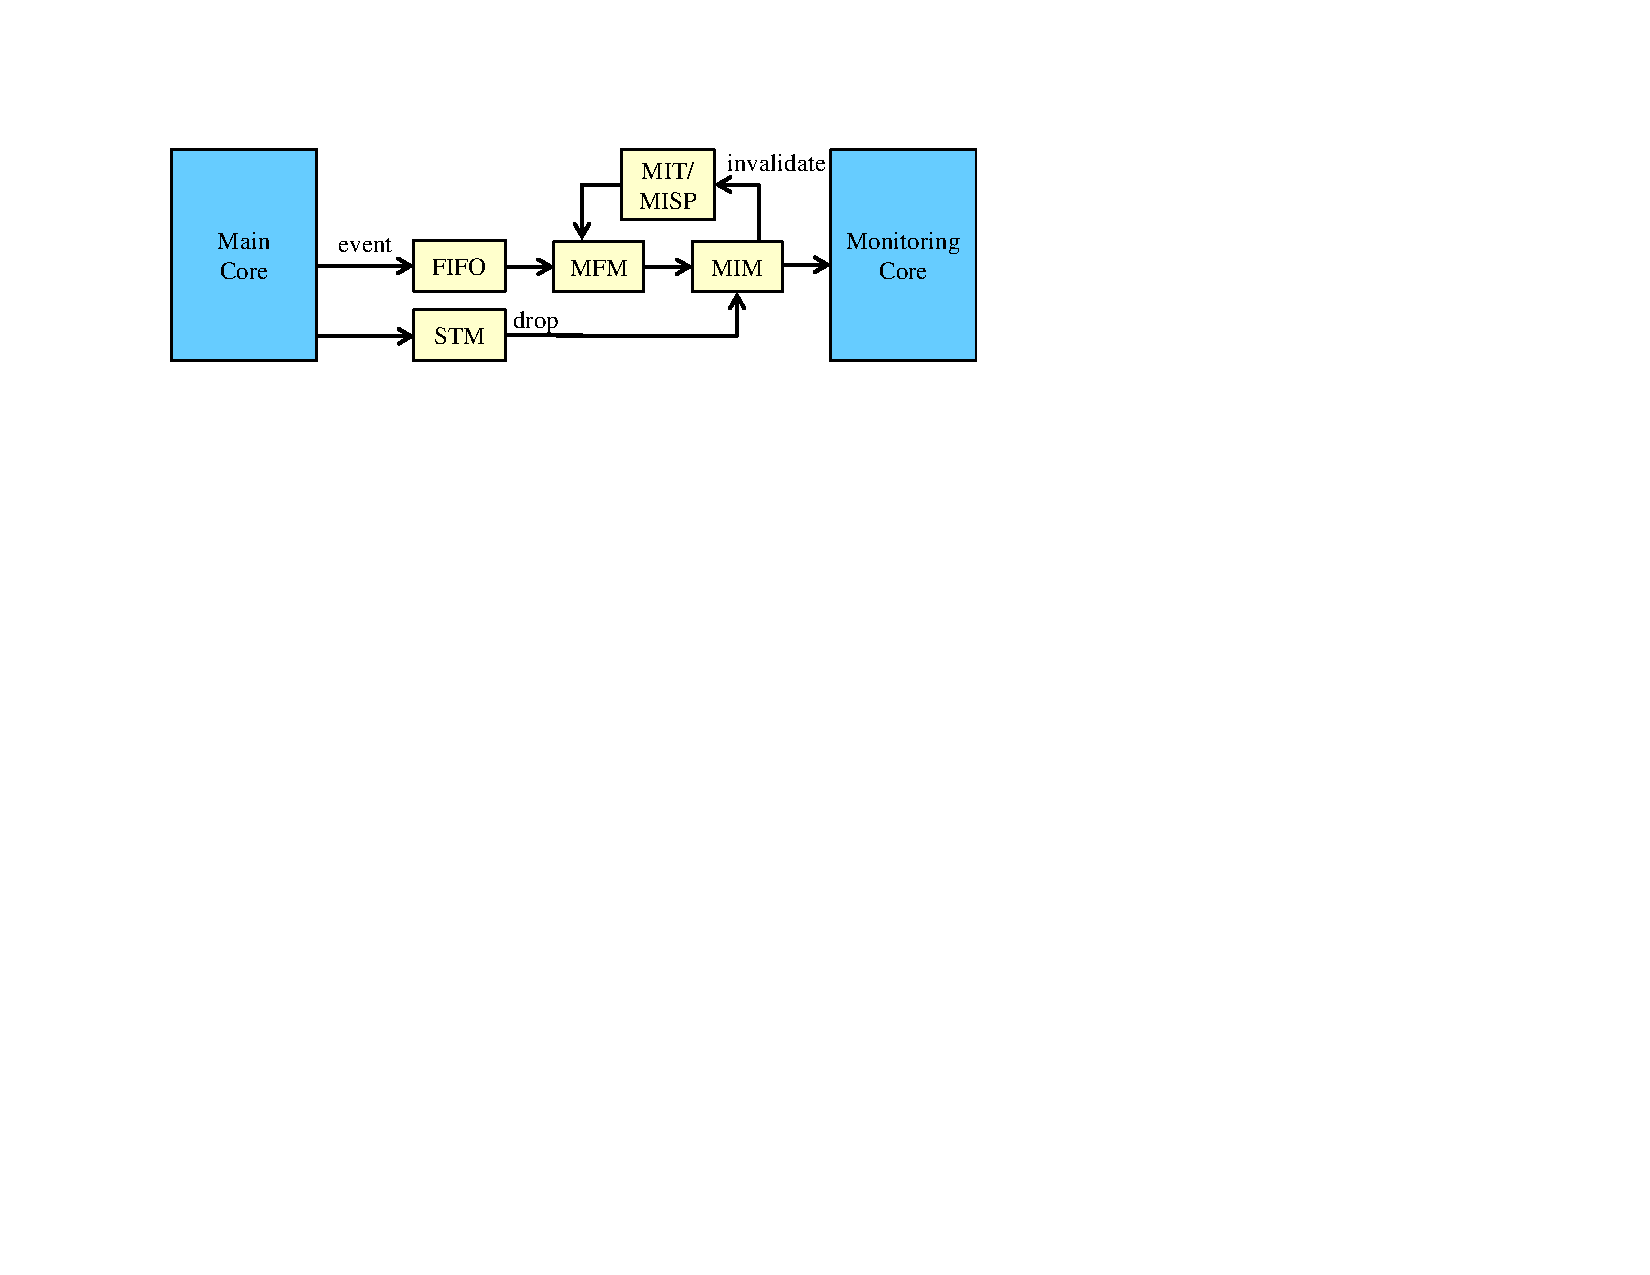
\includegraphics{monitoring_hard_drop/figs/full_hw.pdf}
    \caption{Block diagram of full hardware architecture for opportunistic
    monitoring on hard real-time systems.}
    \label{fig:monitoring_hard_drop.hwdrop.full_hw}
  \end{center}
\end{figure}

Figure~\ref{fig:monitoring_hard_drop.hwdrop.full_hw} shows a block diagram of the complete
architecture.  Monitoring events from the main core are first enqueued in a
FIFO. The events in the FIFO are dequeued and processed by the metadata
filtering module. The MFM checks the MIT and/or MISP to decide whether the
event should be filtered because of invalid metadata. If the event is not
filtered, then the metadata invalidation module decides whether to drop the
event based on the slack tracking module. If the event is dropped or filtered,
then the MIM marks invalidation flags using the MIT/MISP. Instead, if the event
is not dropped or filtered, then it is forwarded to the monitoring core to
perform the monitoring task.

% \section{Evaluation}
\label{sec:monitoring_hard_drop.evaluation}

\subsection{Methodology} 
\label{sec:monitoring_hard_drop.evaluation.methodology}

We implemented our monitoring architecture for real-time systems by modifying
the ARM version of the gem5 simulator \cite{gem5} to support parallel hardware
monitoring and our hardware optimizations for opportunistic monitoring. In
order to explore the generality of the architecture for different monitors, we
implemented the three different monitors: uninitialized memory check (UMC),
return address check (RAC), and dynamic information flow tracking (DIFT).
Uninitialized memory check was mentioned in
Section~\ref{sec:monitoring_wcet.monitoring} and seeks to detect loading from
memory locations that are not initialized first. Return address check protects
against certain security attacks, such as return-oriented programming
\cite{rop-ccs07}, by checking that the address returned to after a
function completes matches the address that originally called the function.
Dynamic information flow tracking is another security monitoring scheme. DIFT
attempts to detect when information from untrusted sources is used to affect
the program control flow. The details of how each of these monitoring schemes
works with our architecture is discussed in the Appendix. We tested our system
using several benchmarks from the M{\"a}lardalen WCET benchmark suite
\cite{malardalen}. 

% Size of memory structures: FIFO, MIT, MISP
We model the main and monitoring cores as 500 MHz in-order cores, each with 16
KB of L1 I/D-caches. The latency to main memory is 15 ns. This setup is
similar to Freescale's i.MX353 processor which targets embedded, automotive,
and industrial applications. For our experiments, we used a FIFO of 16 entries
connecting the main and monitoring cores. The MISP was 16 entries matching the
16 registers found in the ARM architecture. The MIT was configured with 2 ways
and 256 entries. 

% WCET
No static WCET analysis tools exist for the gem5 simulator. In order to
estimate the WCET of tasks, we ran tasks several times on the gem5 simulator
and took the worst-case observed execution time. Our WCET estimate is expected
to be lower than those that a WCET analysis tool would generate since WCET
analysis tools guarantee a conservative estimate. As a result, in our
experiments the gap between actual execution times and our estimated WCET is
lower than what we would expect with a WCET analysis tool. Therefore, the
results we present for the amount of monitoring that can be done are less than
what is expected when a strictly conservative WCET is used.

\subsection{Amount of Monitoring Performed}
\label{sec:monitoring_hard_drop.evaluation.coverage}

% % Full monitoring at zero slack
% \begin{table}
%   \begin{center}
%     \caption{Number of monitored, dropped, and filtered monitoring events as a
%     percentage of the total number of monitoring events. These percentages are
%     shown for zero headstart slack.}
%     \begin{tiny}
%     
% Full monitoring at zero slack

\begin{tabular}{|c|c|c|c|c|c|c|c|c|c|c|}
\hline

\multirow{2}{*}{\bf Monitor} & \multirow{2}{*}{\bf Type} & \multicolumn{8}{c|}{\bf Benchmark} & \multirow{2}{*}{\bf Average} \\ \cline{3-10}
 & & {\tt compress} & {\tt crc} & {\tt edn} & {\tt fir} & {\tt insertsort} & {\tt jfdc} & {\tt nsichneu} & {\tt statemate} & \\ \hline \hline

\multirow{3}{*}{UMC}
& Monitored & 11.9\% & 59.0\% & 4.4\% & 28.4\% & 15.9\% & 16.2\% & 0.0\% & 3.3\% & 17.4\% \\ \cline{2-11}
 & Dropped & 29.4\% & 9.4\% & 5.9\% & 3.9\% & 45.6\% & 43.4\% & 0.13\% & 33.4\% & 21.4\% \\ \cline{2-11}
 & Filtered & 58.7\% & 31.6\% & 89.7\% & 67.7\% & 38.6\% & 40.4\% & 99.9\% & 63.3\% & 61.2\% \\

\hline
\hline

\multirow{3}{*}{RAC} 
 & Monitored & 93.8\% & 50.0\% & 83.3\% & 90.9\% & - & 0.0\% & - & 80.0\% & 66.3\% \\ \cline{2-11}
  & Dropped & 3.1\% & 25.0\% & 8.3\% & 4.5\% & - & 50.0\% & - & 10.0\% & 16.8\% \\ \cline{2-11}
   & Filtered & 3.1\% & 25.0\% & 8.3\% & 4.5\% & - & 50.0\% & - & 10.0\% & 16.8\% \\
 
\hline
\hline

\multirow{3}{*}{DIFT} 
 & Monitored & 11.0\% & 92.2\% & 26.7\% & 22.0\% & 61.8\% & 22.1\% & 4.7\% & 10.6\% & 31.4\% \\ \cline{2-11}
  & Dropped & 26.3\% & 0.89\% & 19.6\% & 18.4\% & 16.6\% & 12.6\% & 57.5\% & 65.7\% & 27.2\% \\ \cline{2-11}
   & Filtered & 62.8\% & 6.9\% & 53.7\% & 59.6\% & 21.6\% & 65.2\% & 37.8\% & 23.6\% & 41.4\% \\

\hline

\end{tabular}

%     \end{tiny}
%     \label{tab:monitoring_hard_drop.evaluation.zero_slack}
%   \end{center}
% \end{table}
% 
% % Coverage at zero slack
% \begin{table}
%   \begin{center}
%     \caption{Percentage of checks that are not dropped or filtered. These percentages are shown for zero headstart slack.}
%     \label{tab:monitoring_hard_drop.evaluation.zero_slack_coverage}
%     \begin{tiny}
%     
% Full monitoring at zero slack

\begin{tabular}{|c|c|c|c|c|c|c|c|c|c|}
\hline

\multirow{2}{*}{\bf Monitor} & \multicolumn{8}{c|}{\bf Benchmark} & \multirow{2}{*}{\bf Average} \\ \cline{2-9}
 & {\tt compress} & {\tt crc} & {\tt edn} & {\tt fir} & {\tt insertsort} & {\tt jfdc} & {\tt nsichneu} & {\tt statemate} & \\ \hline \hline

 UMC & 0.0\% & 59.9\% & 0.41\% & 27.8\% & 10.9\% & 16.3\% & 0.0\% & 0.41\% & 14.5\% \\\hline
 RAC & 93.8\% & 50.0\% & 83.3\% & 90.9\% & - & 0.0\% & - & 80.0\% & 66.3\% \\\hline
 DIFT & 3.8\% & 66.7\% & 44.4\% & 16.7\% & 100.0\% & 100.0\% & 100.0\% & 43.3\% & 59.4\% \\\hline

\end{tabular}

%     \end{tiny}
%   \end{center}
% \end{table}

% Monitoring event breakdown for UMC
\begin{figure}
  \begin{center}
    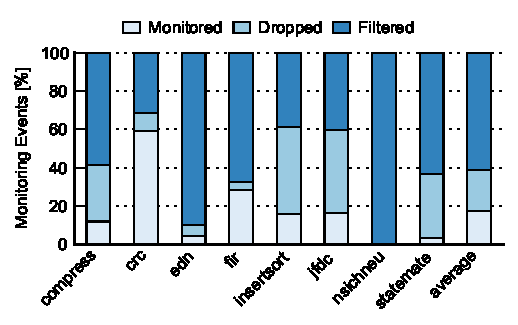
\includegraphics{monitoring_hard_drop/data/zero_slack_umc.pdf}
    \caption{Percentage of monitored, dropped, and filtered monitoring events
    for UMC with zero headstart slack.}
    \label{fig:monitoring_hard_drop.evaluation.zero_slack_umc}
  \end{center}
\end{figure}
% Monitoring event breakdown for LRC
\begin{figure}
  \begin{center}
    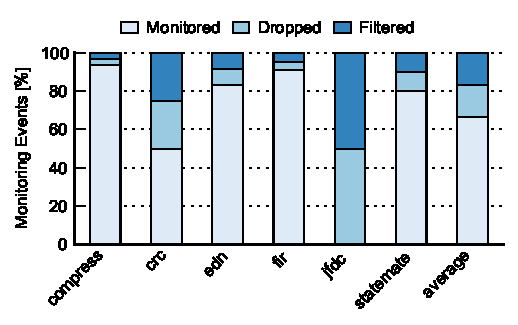
\includegraphics{monitoring_hard_drop/data/zero_slack_lrc.pdf}
    \caption{Percentage of monitored, dropped, and filtered monitoring events
    for RAC with zero headstart slack.}
    \label{fig:monitoring_hard_drop.evaluation.zero_slack_lrc}
  \end{center}
\end{figure}
% Monitoring event breakdown for UMC
\begin{figure}
  \begin{center}
    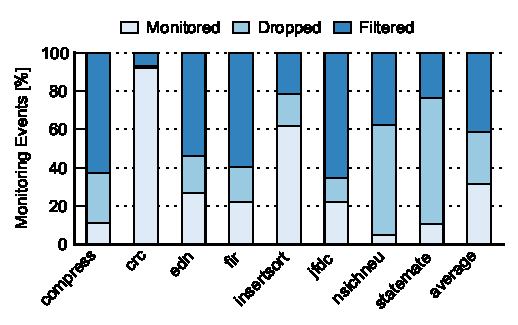
\includegraphics{monitoring_hard_drop/data/zero_slack_dift.pdf}
    \caption{Percentage of monitored, dropped, and filtered monitoring events
    for DIFT with zero headstart slack.}
    \label{fig:monitoring_hard_drop.evaluation.zero_slack_dift}
  \end{center}
\end{figure}

% Coverage
\begin{figure}
  \begin{center}
    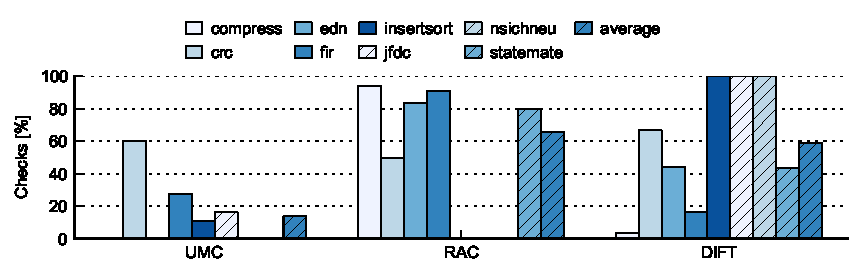
\includegraphics{monitoring_hard_drop/data/zero_slack_coverage.pdf}
    \caption{Percentage of checks that are not dropped or filtered for zero
    headstart slack.}
    \label{fig:monitoring_hard_drop.evaluation.zero_slack_coverage}
  \end{center}
\end{figure}

%In this section, we first present results using only the STM and MIM. The MFM
%is not enabled.
Table~\ref{tab:monitoring_hard_drop.evaluation.zero_slack} shows the number of
monitoring events that are monitored, dropped, and filtered as a percentage of
the total number of monitoring events. We find that a portion of monitoring can
still be done without exceeding the main task's WCET. This is due to the
dynamic slack that is gained during run time. On average, UMC can perform 17\%
of its monitoring tasks. RAC can perform 66\% of its monitoring and DIFT can
perform 31\% of its monitoring.  No results are shown for {\tt insertsort} and
{\tt nsichneu} for RAC because these benchmarks do not make any function calls.
For DIFT, we store the actual DIFT register file metadata in the MISP instead
of invalidation flags. This optimization allows us to use the MIM and MFM to
perform certain monitoring tasks (see Section~\ref{sec:extensions.dift} of the
Appendix for details). These correct metadata updates are counted as
``Monitored'' in the statistics while events are counted as dropped or filtered
only if they were due to insufficient slack.

As expected, a false positive never occurred in our experiments. However, false
negatives can occur due to dropping monitoring tasks. Specifically, dropped or
filtered check-type monitoring operations can result in false negatives.
Table~\ref{tab:monitoring_hard_drop.evaluation.zero_slack_coverage} shows the
number of checks that are monitored as a percentage of the total checks. This
acts as a measure of the coverage achieved by the monitors. The coverage for
UMC is 15\% on average and the coverage for RAC is 66\% on average. The average
coverage for DIFT is 59\% which is much higher than the percentage of
monitoring tasks that are not dropped or filtered. In fact, for some of the
benchmarks, DIFT is able to achieve 100\% coverage. This implies that only a
portion of the monitoring operations performed by DIFT actually affect the
checks.  For example, DIFT propagates metadata on every ALU, load, and store
instruction. However, only instructions that eventually propagate metadata to
an indirect jump instruction affect the coverage.

% Coverage for UMC
\begin{figure}
  \begin{center}
    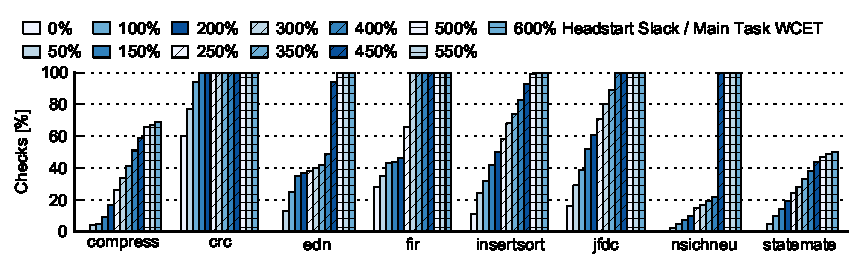
\includegraphics{monitoring_hard_drop/data/umc_sweep.pdf}
    \caption{Percentage of checks performed as headstart slack is varied for
    UMC. Headstart slack is shown normalized to the main task's WCET.}
    \label{fig:monitoring_hard_drop.evaluation.umc_sweep}
  \end{center}
\end{figure}

% Coverage DIFT
\begin{figure}
  \begin{center}
    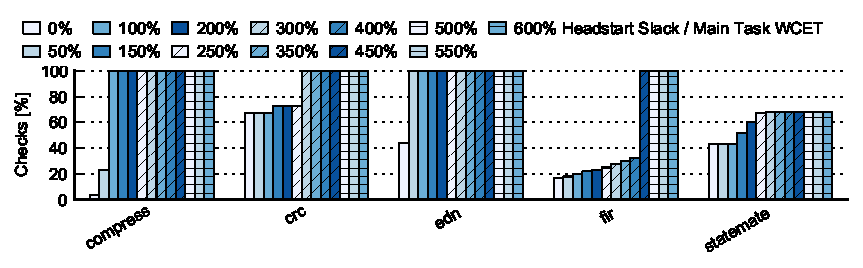
\includegraphics{monitoring_hard_drop/data/dift_sweep.pdf}
    \caption{Percentage of checks performed as headstart slack is varied for
    DIFT. Headstart slack is shown normalized to the main task's WCET.}
    \label{fig:monitoring_hard_drop.evaluation.dift_sweep}
  \end{center}
\end{figure}

For an underutilized system, if some headstart slack is given to a task
initially, then the amount of monitoring that can be performed can be
increased. As an example,
Figure~\ref{fig:monitoring_hard_drop.evaluation.umc_sweep} shows how the
coverage increases as we increase the headstart slack given to the main task
for UMC. Figure~\ref{fig:monitoring_hard_drop.evaluation.dift_sweep} shows how
the coverage varies with headstart slack for DIFT. Results for RAC are similar
and can be found in Section~\ref{sec:appendix.rac} of the Appendix.  The
headstart slack is displayed as a percentage of the main task's WCET for each
benchmark and is varied from 0\% to 600\%. With enough headstart slack, 100\%
of the monitoring is able to be performed. For DIFT, only benchmarks which were
not able to reach 100\% coverage with zero headstart slack are shown.  {\tt
compress} and {\tt statemate} do not reach 100\% coverage across the varied
range. This is not surprising as both had especially high WCET for performing
monitoring without dropping (see
Figure~\ref{fig:monitoring_hard_drop.drop.sw_drop_wcet}). With higher headstart
slack, these benchmarks should also reach 100\% coverage.

% Coverage for LRC
\begin{figure}
  \begin{center}
    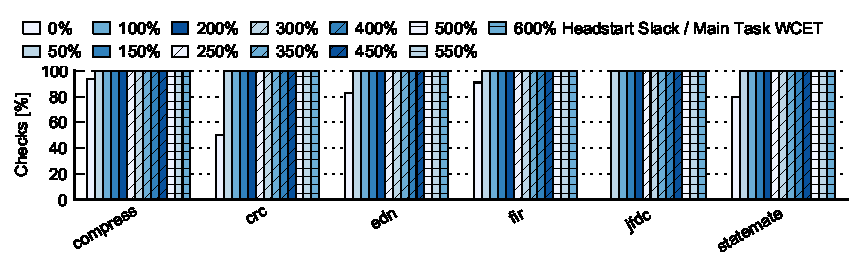
\includegraphics{monitoring_hard_drop/data/lrc_sweep.pdf}
    \caption{Percentage of checks performed as headstart slack is varied for
    RAC implemented on a processor core. Headstart slack is shown normalized
    to the main task's WCET.}
    \label{fig:monitoring_hard_drop.evaluation.lrc_sweep}
  \end{center}
\end{figure}

\begin{figure}
  \begin{center}
    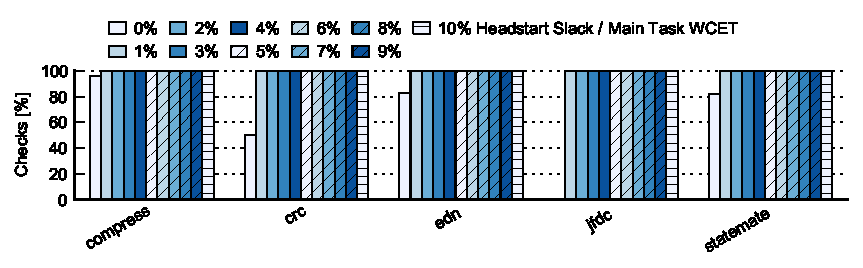
\includegraphics{monitoring_hard_drop/data/flex_lrc_sweep.pdf}
    \caption{Percentage of checks performed as headstart slack is varied for
    RAC on an FPGA-based monitor. Headstart slack is shown normalized to the
    main task's WCET.}
    \label{fig:monitoring_hard_drop.evaluation.flex_lrc_sweep}
  \end{center}
\end{figure}

This section shows how the coverage varies as headstart slack is changed for
RAC. Figure~\ref{fig:monitoring_hard_drop.evaluation.lrc_sweep} shows the
coverage for a processor core implementation of RAC while
Figure~\ref{fig:monitoring_hard_drop.evaluation.flex_lrc_sweep} shows the
coverage for an FPGA-based monitor. {\tt insertsort} and {\tt nsichneu} were
omitted as they do not perform function calls. {\tt fir} is not shown for the
FPGA-based monitor because it already achieves 100\% coverage with zero
headstart slack. In both cases, we see that with a small amount of headstart
slack, RAC is able to reach 100\% coverage for all benchmarks.

\subsection{FPGA-based Monitor}
\label{sec:monitoring_hard_drop.evaluation.fpga}

% % Full monitoring at zero slack on Flex
% \begin{table}[tb]
%   \begin{center}
%     \caption{Number of monitored, dropped, and filtered monitoring events as a
%     percentage of the total number of monitoring events for an FPGA-based
%     monitor. These percentages are shown for zero headstart slack.}
%     \begin{footnotesize}
%     
% Full monitoring at zero slack on Flex

\begin{tabular}{|c|c|c|c|c|c|c|c|c|c|c|}
\hline

\multirow{2}{*}{\bf Monitor} & \multirow{2}{*}{\bf Type} & \multicolumn{8}{c|}{\bf Benchmark} & \multirow{2}{*}{\bf Average} \\ \cline{3-10}
 & & {\tt compress} & {\tt crc} & {\tt edn} & {\tt fir} & {\tt insertsort} & {\tt jfdc} & {\tt nsichneu} & {\tt statemate} & \\ \hline \hline

\multirow{3}{*}{UMC}
  & Monitored & 29.6\% & 85.9\% & 97.3\% & 83.3\% & 91.4\% & 88.7\% & 14.5\% & 45.7\% & 67.1\% \\ \cline{2-11}
   & Dropped & 17.4\% & 3.3\% & 0.05\% & 2.7\% & 3.0\% & 3.1\% & 0.10\% & 8.5\% & 4.8\% \\ \cline{2-11}
    & Filtered & 53.0\% & 10.8\% & 2.7\% & 14.0\% & 5.6\% & 8.3\% & 85.4\% & 45.8\% & 28.2\% \\

\hline
\hline

\multirow{3}{*}{RAC} 
 & Monitored & 94.8\% & 50.0\% & 83.3\% & 95.5\% & - & 0.0\% & - & 81.0\% & 67.4\% \\ \cline{2-11}
  & Dropped & 3.1\% & 25.0\% & 8.3\% & 4.5\% & - & 50.0\% & - & 10.0\% & 16.8\% \\ \cline{2-11}
   & Filtered & 2.1\% & 25.0\% & 8.3\% & 0.0\% & - & 50.0\% & - & 9.0\% & 15.7\% \\
 
\hline
\hline

\multirow{3}{*}{DIFT} 
 & Monitored & 40.6\% & 97.6\% & 64.7\% & 50.6\% & 97.9\% & 75.8\% & 96.6\% & 51.5\% & 71.9\% \\ \cline{2-11}
  & Dropped & 8.8\% & 0.06\% & 13.6\% & 0.91\% & 0.97\% & 0.95\% & 2.1\% & 33.6\% & 7.6\% \\ \cline{2-11}
   & Filtered & 50.6\% & 2.3\% & 21.7\% & 48.5\% & 1.1\% & 23.3\% & 1.3\% & 14.9\% & 20.5\% \\

\hline

\end{tabular}

%     \end{footnotesize}
%     \label{tab:monitoring_hard_drop.evaluation.zero_slack_flex}
%   \end{center}
% \end{table}
% 
% % Full monitoring at zero slack on Flex
% \begin{table}[tb]
%   \begin{center}
%     \caption{Percentage of checks that are not dropped or filtered for an
%     FPGA-based monitor. These percentages are shown for zero headstart slack.}
%     \label{tab:monitoring_hard_drop.evaluation.zero_slack_flex_coverage}
%     \begin{footnotesize}
%     
% Full monitoring at zero slack

\begin{tabular}{|c|c|c|c|c|c|c|c|c|c|}
\hline

\multirow{2}{*}{\bf Monitor} & \multicolumn{8}{c|}{\bf Benchmark} & \multirow{2}{*}{\bf Average} \\ \cline{2-9}
 & {\tt compress} & {\tt crc} & {\tt edn} & {\tt fir} & {\tt insertsort} & {\tt jfdc} & {\tt nsichneu} & {\tt statemate} & \\ \hline \hline

UMC & 9.9\% & 87.8\% & 97.1\% & 85.1\% & 86.1\% & 84.8\% & 14.5\% & 28.3\% & 61.7\% \\\hline
RAC & 95.8\% & 50.0\% & 83.3\% & 100.0\% & - & 0.0\% & - & 82.0\% & 68.5\% \\\hline
DIFT & 3.8\% & 93.3\% & 100.0\% & 100.0\% & 100.0\% & 100.0\% & 100.0\% & 88.3\% & 85.7\% \\\hline

\end{tabular}

%     \end{footnotesize}
%   \end{center}
% \end{table}

% Monitoring event breakdown for UMC
\begin{figure}
  \begin{center}
    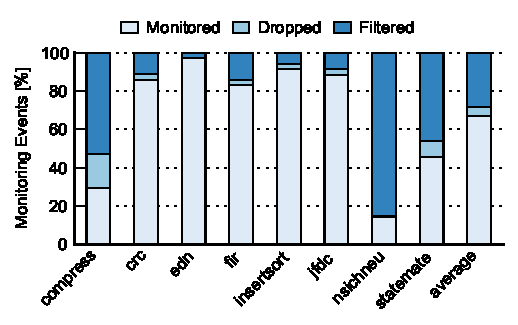
\includegraphics{monitoring_hard_drop/data/zero_slack_flex_umc.pdf}
    \caption{Percentage of monitored, dropped, and filtered monitoring events
    for UMC on an FPGA-based monitor with zero headstart slack.}
    \label{fig:monitoring_hard_drop.evaluation.zero_slack_flex_umc}
  \end{center}
\end{figure}
% Monitoring event breakdown for LRC
\begin{figure}
  \begin{center}
    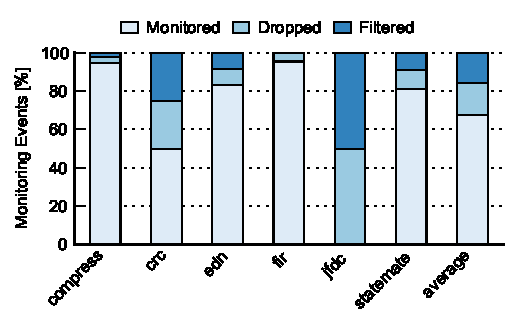
\includegraphics{monitoring_hard_drop/data/zero_slack_flex_lrc.pdf}
    \caption{Percentage of monitored, dropped, and filtered monitoring events
    for RAC on an FPGA-based monitor with zero headstart slack.}
    \label{fig:monitoring_hard_drop.evaluation.zero_slack_flex_lrc}
  \end{center}
\end{figure}
% Monitoring event breakdown for UMC
\begin{figure}
  \begin{center}
    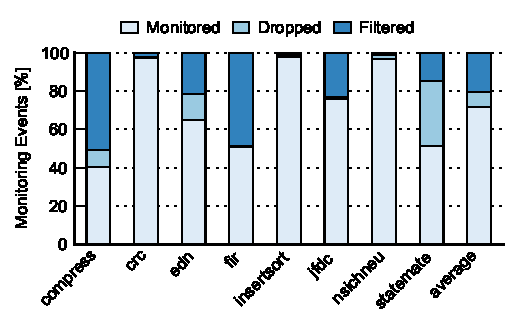
\includegraphics{monitoring_hard_drop/data/zero_slack_flex_dift.pdf}
    \caption{Percentage of monitored, dropped, and filtered monitoring events
    for DIFT on an FPGA-based monitor with zero headstart slack.}
    \label{fig:monitoring_hard_drop.evaluation.zero_slack_flex_dift}
  \end{center}
\end{figure}

% Coverage
\begin{figure}
  \begin{center}
    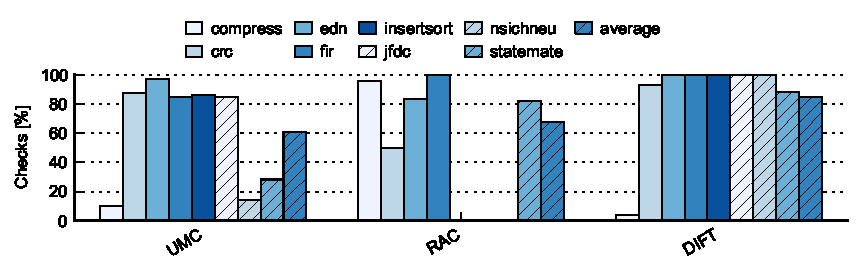
\includegraphics{monitoring_hard_drop/data/zero_slack_flex_coverage.pdf}
    \caption{Percentage of checks that are not dropped or filtered on an
    FPGA-based monitor for zero headstart slack.}
    \label{fig:monitoring_hard_drop.evaluation.zero_slack_flex_coverage}
  \end{center}
\end{figure}

Performing monitoring in software, although parallelized, can still incur high
overheads since multiple instructions are needed to handle each monitoring
event. One possible solution to improve the performance of monitoring while
maintaining programmability is to use an FPGA-based monitor
\cite{flexcore-micro10}. We model the FPGA-based monitor as being able to
run at 250 MHz and handle up to one monitoring event each cycle. Note that this
means that the FPGA-based monitor can process a monitoring event every two
cycles of the main core which runs at 500 MHz.
Table~\ref{tab:monitoring_hard_drop.evaluation.zero_slack_flex} shows the
number of monitored, dropped, and filtered events with no headstart slack for
this FPGA-based monitor. UMC and RAC are able to run 67\% of their monitoring
tasks on average, while DIFT is able to run 72\% of its monitoring tasks on
average.
Table~\ref{tab:monitoring_hard_drop.evaluation.zero_slack_flex_coverage} shows
the coverage achieved by these monitoring schemes on an FPGA-based monitor. RAC
shows similar numbers to processor-based monitoring because the number of calls
and returns in these benchmarks is relatively small. However, for UMC and DIFT,
we see that an FPGA-based monitor allows much more monitoring to be done
without increasing the headstart slack. The coverage for UMC increases from
15\% to 62\% while the coverage for DIFT increases from 59\% to 86\%.

\begin{figure}
  \begin{center}
    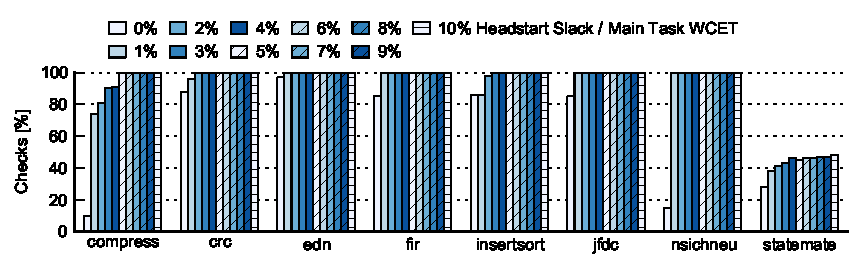
\includegraphics{monitoring_hard_drop/data/flex_umc_sweep.pdf}
    \caption{Percentage of checks performed as headstart slack is varied for
    UMC on an FPGA-based monitor. Headstart slack is shown normalized to the
    main task's WCET.}
    \label{fig:monitoring_hard_drop.evaluation.flex_umc_sweep}
  \end{center}
\end{figure}

\begin{figure}
  \begin{center}
    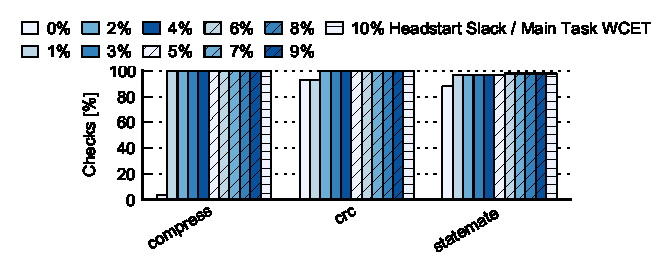
\includegraphics{monitoring_hard_drop/data/flex_dift_sweep.pdf}
    \caption{Percentage of checks performed as headstart slack is varied for
    DIFT on an FPGA-based monitor. Headstart slack is shown normalized to the
    main task's WCET.}
    \label{fig:monitoring_hard_drop.evaluation.flex_dift_sweep}
  \end{center}
\end{figure}

Figure~\ref{fig:monitoring_hard_drop.evaluation.flex_umc_sweep} shows how the
coverage for UMC varies as we increase the headstart slack from 0\% to 10\% for
an FPGA-based monitor.
Figure~\ref{fig:monitoring_hard_drop.evaluation.flex_dift_sweep} shows this
data for DIFT and results for RAC can be found in
Section~\ref{sec:appendix.rac} of the Appendix.  We can see that for a
high-performance FPGA-based monitor, with a small amount of slack, we are able
to achieve 100\% monitoring for almost all benchmarks while guaranteeing the
main task's execution time does not exceed its WCET. 

\subsection{Area and Power Overheads}

% Area and Power Overheads
\begin{table}[tb]
  \begin{center}
    \caption{Average power overheads for dropping hardware at zero headstart
    slack. Percentages in parentheses are normalized to the main core's power usage.}
    \begin{footnotesize}
    
% Full monitoring at zero slack

\begin{tabular}{|c|c|c|c|}
\hline

\multicolumn{2}{|c|}{\bf Monitor} & {\bf Peak Power [mW]} & {\bf Runtime Power [mW]} \\ \hline\hline

\multirow{3}{*}{Processor} 
& UMC  & 4.9 (3.2\%) & 4.7 (6.6\%) \\ \cline{2-4}
& RAC  & 4.7 (3.1\%) & 4.7 (6.6\%) \\ \cline{2-4}
& DIFT & 5.0 (3.3\%) & 4.8 (6.7\%) \\ \hline\hline

\multirow{3}{*}{FPGA} 
& UMC  & 16.7 (10.9\%) & 8.5 (11.9\%) \\ \cline{2-4}
& RAC  &  4.7  (3.1\%) & 4.7  (6.6\%) \\ \cline{2-4}
& DIFT & 13.0  (8.5\%) & 8.8 (12.3\%) \\ \hline

\end{tabular}

    \end{footnotesize}
    \label{tab:monitoring_hard_drop.evaluation.area_power}
  \end{center}
\end{table}

Adding the dropping hardware in order to enable adjustable overheads adds
overheads in terms of area and power. We use McPAT \cite{mcpat-micro09} to get
a first-order estimate of these area and power overheads in a 40 nm technology
node. McPAT estimates the main core area as 1.96 mm$^2$ and the peak power
usage as 152.9 mW averaged across all benchmarks. The average runtime power
usage was 71.6 mW. These area and power numbers consist of the core and L1
cache, but do not include memory controllers and other peripherals. The power
numbers include dynamic as well as static (leakage) power. For the dropping
hardware, the ALUs, MISP, MIT, and configuration tables are modeled using the
corresponding objects in McPAT. We note that this is only a rough area and
power result since components such as the wires connecting these modules have
not been modeled. However, this gives a sense of the order-of-magnitude
overheads involved with implementing our approach.

An additional 0.132 mm$^2$ of silicon area is needed, an increase of 7\% of the
main core area. Table~\ref{tab:monitoring_hard_drop.evaluation.area_power}
shows the peak and runtime power overheads with zero headstart slack for both a
processor-based monitor as well as an FPGA-based monitor. The peak power is
5-17 mW, which is 3-11\% of the main core's peak power usage. The average
runtime power is 5-9 mW, corresponding to 7-12\% of the main core's runtime
power. For UMC and DIFT, the core-based monitor has lower power usage due to
more monitoring events being filtered out that do not require invalidation.
This reduces the activity of the Metadata Invalidation Module which reduces the
power usage.



\chapter{Run-Time Monitoring with Adjustable Overheads Using Dataflow-Guided Filtering}
\label{chap:monitoring_dift_drop}

\section{Introduction}
\label{sec:monitoring_dift_drop.introduction}

In the last chapter, we described a hardware architecture that dynamically
limits the amount of monitoring performed in order to meet hard real-time
deadlines. This allows run-time monitoring to be implemented even when the
worst-case impact of performing full monitoring cannot be tolerated. 
For some of these monitoring techniques, even the average or typical case
overheads can be prohibitively high depending on the application and system
requirements.  Thus, in this chapter, we explore the use of similar hardware
techniques in order to enable a new trade-off dimension for run-time monitoring
designs.  We propose to enable low overhead monitors by using partial
monitoring. This enables a trade-off between overhead and
monitoring coverage or accuracy. 

We enable partial monitoring with adjustable overhead by dynamically dropping
monitoring operations when the overhead exceeds a specified overhead budget.
Similar to the architecture presented in
Chapter~\ref{chap:monitoring_hard_drop}, we must again be careful to prevent
false positives due to out-of-date metadata information. In order to prevent
these false positives, we use an invalidation-based approach as before.
However, here we back up the invalidation flags to memory and do not have
aliasing. The result is that the hardware effectively acts as a dataflow
tracking engine. We show how a simple extension to this dataflow engine can
enable null metadata filtering. In addition, we investigate different policies
for deciding which events to drop for partial monitoring.  These different
policies show a trade-off between closely matching the overhead budget and
increasing the monitoring coverage.

This chapter is organized as follows.
Section~\ref{sec:monitoring_dift_drop.monitoring} introduces the notion of
adjustable overhead through partial monitoring.
Section~\ref{sec:monitoring_dift_drop.dropping} discusses the hardware
architecture that enables partial monitoring using our dataflow tracking
engine.  Section~\ref{sec:monitoring_dift_drop.policies} investigates the
design space for dropping policies that determine when and which monitoring
operations to drop.  Section~\ref{sec:monitoring_dift_drop.evaluation} presents
our evaluation methodology and results. 


\section{Partial Run-Time Monitoring}
\label{sec:monitoring_dift_drop.monitoring}

% Previous work overheads
\begin{table}
  \begin{center}
    \begin{tiny}
    %\begin{tabular}{|l|p{2in}|r|r|}
\begin{tabular}{|l|l|l|r|}

\hline
{\bf Name} & {\bf Type} & {\bf Monitoring scheme and flexibility} & {\bf Slowdown (avg./worst)} \\ \hline\hline

% DIFT \cite{dift-asplos04} & Custom HW & DIFT only & 1.1\% / 23\% \\ \hline
% FlexiTaint \cite{flexitaint-hpca08} & Custom HW & DIFT w/ programmable policies & 1.1\%-3.7\% / 8.7\% \\ \hline
% Hardbound \cite{hardbound-asplos08} & Custom HW & Array bounds checks only & 5\%-9\% / 22\% \\ \hline
% Harmoni \cite{harmoni-dsn12} & Custom HW & Tag-based monitors & 1\%-10\% / 20\% \\ \hline\hline

DIFT \cite{dift-asplos04} & Custom HW & DIFT only & 1.01x / 1.23x \\ \hline
FlexiTaint \cite{flexitaint-hpca08} & Custom HW & DIFT w/ programmable policies & 1.01x-1.04x / 1.09x \\ \hline
Hardbound \cite{hardbound-asplos08} & Custom HW & Array bounds checks only & 1.05x-1.09x / 1.22x \\ \hline
Harmoni \cite{harmoni-dsn12} & Custom HW & Tag-based monitors & 1.01x-1.10x / 1.20x \\ \hline\hline

FlexCore \cite{flexcore-micro10} & Dedicated FPGA & Instruction-trace monitoring & 1.05x-1.44x / 1.84x \\ \hline
FADE \cite{fade-hpca14} & Core+Custom HW & Instruction-trace monitoring (effective when HW filters work) & 1.2x-1.8x / 3.3x \\ \hline
LBA-accelerated \cite{lba-isca08} & Multi-core+Custom HW & Instruction-trace monitoring (effective when accelerators work) & 1.02x-3.27x / 5x \\ \hline
LBA \cite{lba-asid06} & Multi-core+Custom HW & Instruction trace monitoring & 3.23x-7.80x / 11x \\ \hline \hline

Multi-core DIFT \cite{nagarajan-interact08} & SW (multithreaded) & DIFT (compiled for each application) & 1.48x / 2.2x \\ \hline

LIFT \cite{lift-micro06} & SW (DBI) & DIFT (fully flexible) & 3.6x / 7.9x \\ \hline
Purfiy \cite{purify-usenix92} & SW (DBI) & Memory leak checks (fully flexible) & 2.3x / 5.5x \\ \hline
TaintCheck \cite{taintcheck-ndsss05} & SW (DBI) & DIFT (fully flexible) & 10x / 27x \\ \hline


\end{tabular}

    \end{tiny}
    \caption{Trade-off between performance overhead and flexibility/complexity
    of run-time monitoring systems.}
    \label{tab:monitoring_dift_drop.monitoring.previous_overheads}
  \end{center}
\end{table}

\subsection{Overhead of Run-Time Monitoring}

There have been a number of proposals for run-time monitoring systems exploring
various design points.
Table~\ref{tab:monitoring_dift_drop.monitoring.previous_overheads} summarizes
some of the representative designs and their reported performance overheads.
The previous studies clearly show that there exist trade-offs between
efficiency, flexibility, and hardware costs.  For example, a run-time
monitoring scheme can often be realized with fairly low performance overhead
(less than 20\%) if implemented with custom hardware that is designed only for
one monitor or a narrow set of monitors. However, the custom hardware monitors
cannot be modified or updated, and require dedicated silicon area.  On the
other hand, flexible systems that support a wide range of monitors lead to
noticeable performance overhead, often too high for wide deployment in
practice.  Software-only implementations \cite{nagarajan-interact08,
lift-micro06, purify-usenix92, taintcheck-ndsss05} or multi-core monitors with
minimal hardware changes \cite{lba-asid06} are reported to have severalfold
slowdowns.  On-chip FPGA monitors \cite{flexcore-micro10} and cores with
monitoring accelerators \cite{lba-isca08, fade-hpca14} can reduce overhead
significantly, but still show slowdowns of several tens of percents in some
cases.  In today's monitoring systems, the overhead is also unpredictable
because it depends heavily on the characteristics of applications and
monitoring operations.  In summary, users currently need to either pay
noticeable overhead or the cost of custom hardware in order to use fine-grained
run-time monitoring in deployed systems.

\subsection{Partial Monitoring for Adjustable Overhead}

In this paper, we aim to develop a general framework that enables monitoring
overhead to be dynamically adjusted by dropping a portion of monitoring
operations if necessary. In essence, this framework adds a new dimension to the
monitor design space by allowing coverage or accuracy to be traded off for
lower overhead. For example, the capability to adjust overhead allows users to
use monitoring with partial coverage in order to reduce performance or energy
overhead. Alternatively, partial monitoring allows designers to use less
expensive hardware for a given performance overhead budget.

In this framework, a user specifies how much monitoring should be done in the
form of a target overhead budget, a target coverage, a percentage of monitoring
operations to be performed, etc.  Then, the framework dynamically drops a
portion of monitoring operations to match the target. In particular, this paper
focuses on matching a performance overhead target while maximizing the
coverage. Given that the overhead of custom hardware monitors can already be
quite low, the focus is on enabling the trade-off in {\em general-purpose}
monitoring systems that support a wide range of monitors.  We also consider the
target overhead as a soft constraint and do not aim to provide a strict
worst-case guarantee.

\subsection{Applications and Metrics}

While it is ideal if run-time monitoring can be performed in full, we believe
that the capability to trade-off coverage/accuracy for lower
performance/hardware overhead will be useful in many application scenarios
where full monitoring is not a viable option.  Here, we briefly discuss example
applications of partial monitoring and the metrics that are important in each
case.

{\bf Cooperative testing, debugging, and protection:} 
Recent studies have shown that software testing, debugging, or attack detection
may be done in a cooperative fashion across a large number of systems
\cite{liblit-pldi05, chilimbi-asplos04, greathouse-cgo11, testudo-micro08}. In
this case, each system is only willing to pay very low overhead (e.g., a few
percent) and only performs a small subset of checks.  High coverage is achieved
by having different systems check different parts of a program.  The partial
monitoring framework allows high-overhead monitoring to be used in a
cooperative fashion.  The main metric that represents the effectiveness of
monitoring in this case is the coverage (the percentage of checks that were
performed) over multiple runs.

{\bf Monitoring of soft real-time systems:}
Soft real-time systems or interactive systems need to meet deadlines or
response-time requirements. Unfortunately, the overhead of run-time monitoring
is often unpredictable and varies significantly depending on the application
and monitor characteristics. The partial monitoring framework allows monitoring
to be performed while providing a level of guarantee on its impact on the
execution time.  In this case, it is important that the system can closely
match the desired overhead target while maximizing the effectiveness of
monitoring.

{\bf Partial protection for low overhead:}
Even without real-time constraints, systems may have tight budgets for the
performance, energy, or hardware overhead that they can tolerate for run-time
monitoring. In such cases, full monitoring cannot be enabled unless its
overhead is low enough. Adjustable monitoring allows partial protection on such
systems. For example, array bounds may be checked for a subset of memory
accesses. For dynamic information flow tracking (DIFT), a subset of information
flows may be tracked for partial attack detection. In this scenario, the
effectiveness of partial monitoring can be measured as the percentage of
run-time checks that are performed on each program run, which reflects how
likely it is for a bug or an attack to be detected for a system. 

{\bf Profiling:} 
The run-time monitoring system can be used to implement various profiling tools
to collect statistics on program behavior for performance optimizations as well
as security protection. For example, a recent study showed that an instruction
mix can be used to identify malware from normal programs \cite{demme-isca13,
tang-raid14}.  In such profiling tools, the partial monitoring framework can be
used to obtain statistical samples rather than complete counts of all program
events, essentially trading off accuracy for lower overhead.

\subsection{Design Challenges}

While conceptually simple, designing a general framework to dynamically adjust
monitoring overhead introduces new challenges that need to be addressed.  The
following summarizes the main design goals and associated design challenges.

\begin{enumerate}
  \item \textbf{General:} Since we mainly target flexible run-time monitoring
  systems, which often have high overhead, the framework also needs to be
  general enough to be applicable to a wide range of monitoring schemes.

  \item \textbf{No false positive:} The framework needs to ensure that dropping
  a portion of monitoring operations does not lead to a false positive. We
  found that a dataflow engine that tracks invalid metadata can serve as a
  general solution to this problem
  (Section~\ref{sec:monitoring_dift_drop.dropping}).

  \item \textbf{Intelligent dropping:} The framework needs to match the
  overhead budget while maximizing the effectiveness of monitoring. To this
  end, partial monitoring needs to carefully choose which operations to drop
  and when. We address this problem by studying different dropping policies
  (Section~\ref{sec:monitoring_dift_drop.policies}) and their trade-offs.
\end{enumerate}


\section{Architecture for Partial Monitoring}
\label{sec:monitoring_dift_drop.dropping}

% Example monitor
\begin{figure}
  \begin{center}
    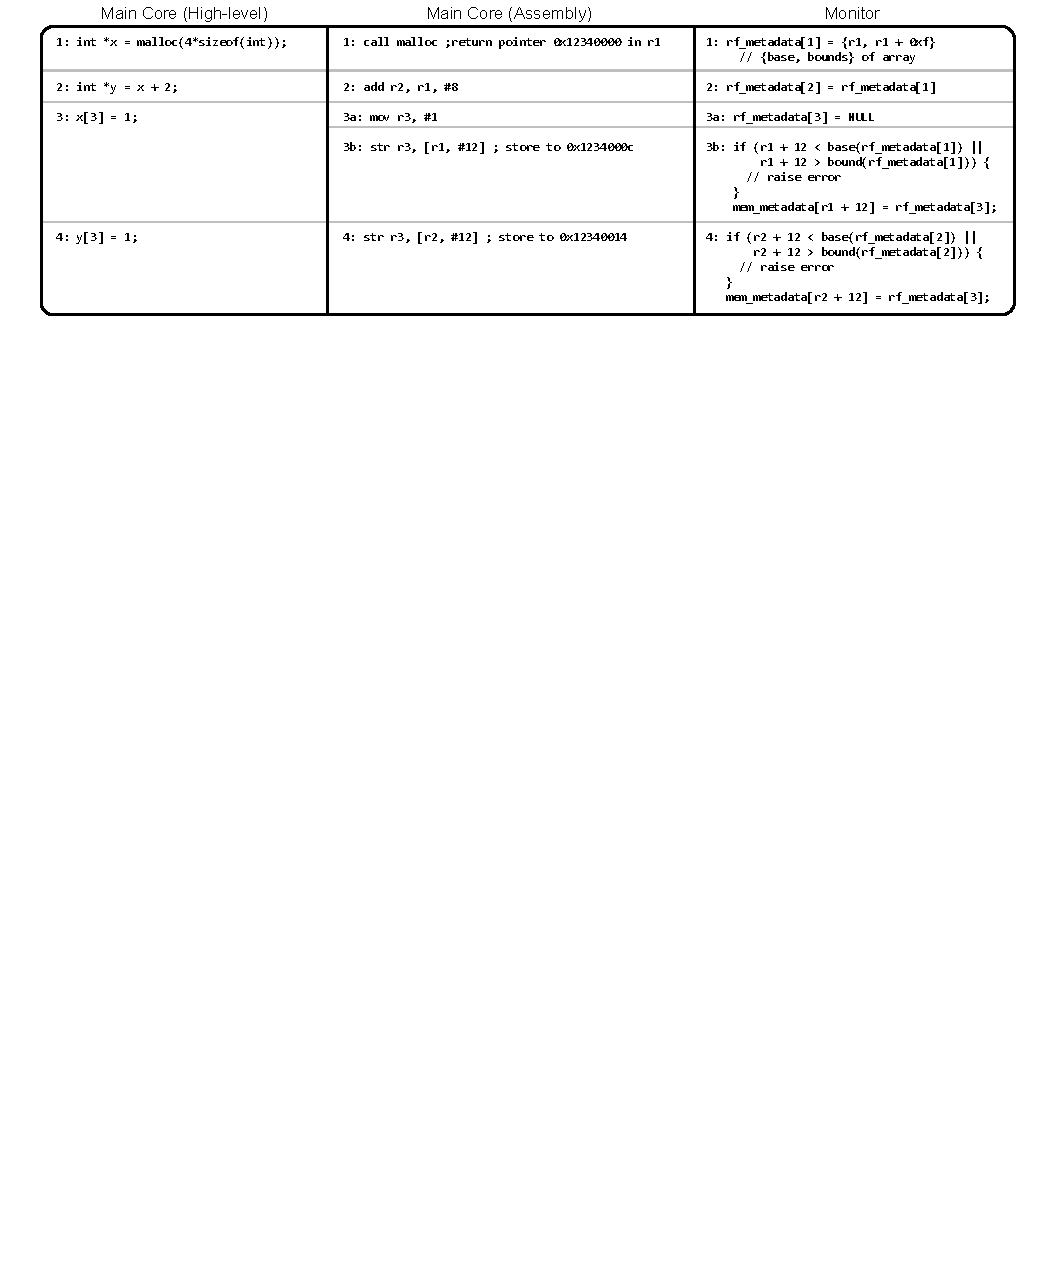
\includegraphics{monitoring_wcet/figs/example_full.pdf}
    \caption{Example of array bounds check monitor.}
    \label{fig:monitoring_dift_drop.dropping.example_full}
  \end{center}
\end{figure} 

In this section, we present our hardware architecture that enables partial
monitoring for adjustable overhead. We will revisit the array bounds check
monitor and example code sequence that was shown in
Figure~\ref{fig:monitoring_wcet.monitoring.example_full} from
Section~\ref{sec:monitoring_wcet.monitoring.example}. This example is repeated
in Figure~\ref{fig:monitoring_dift_drop.dropping.example_full} for easy
reference.

\subsection{Effects of Dropping Monitoring}
\label{sec:monitoring_dift_drop.dropping.false_neg_pos}

Our goal is to drop some monitoring operations in order to reduce the overhead
of run-time monitoring. This dropping can affect the functionality of the
monitoring scheme. There are three possible outcomes for dropping a monitoring
operation. The first is that there is no difference in operation from the
original execution. For example, if we drop line 3b from our array bounds check
example (Figure~\ref{fig:monitoring_dift_drop.dropping.example_full}), then the
check on accessing {\tt x+12} is skipped. However, this is a valid access and
so skipping the check does not change anything.

On the other hand, if the monitoring for accessing memory location {\tt y+12}
on line 4 is skipped, then a false negative occurs. Originally, the monitor
would catch this access as an out-of-bounds access and raise an error. However,
if the monitoring operation for this is dropped, then the error is not
detected. This reflects the trade-off that we make in order to reduce overhead.
Instead of either 100\% coverage with all the associated overhead or no
coverage and no overhead, we enable middle points of partial coverage with some
fraction of the full overhead.

The final possible outcome of dropping a monitoring operation is a false
positive.  For example, suppose the monitoring for line 1 is dropped, causing
the bound information for pointer {\tt x} to never be set. The result is that
when the access using {\tt x} is checked on line 3b, an error will be raised.
This creates a false positive where an error is incorrectly raised. Although
false negatives are part of the trade-off we make to reduce overhead, we need
to prevent false positives.

\subsection{Invalidation for Preventing False Positives}
\label{sec:monitoring_dift_drop.dropping.prevent_false_pos}

% Example with invalidation
\begin{figure}
  \begin{center}
    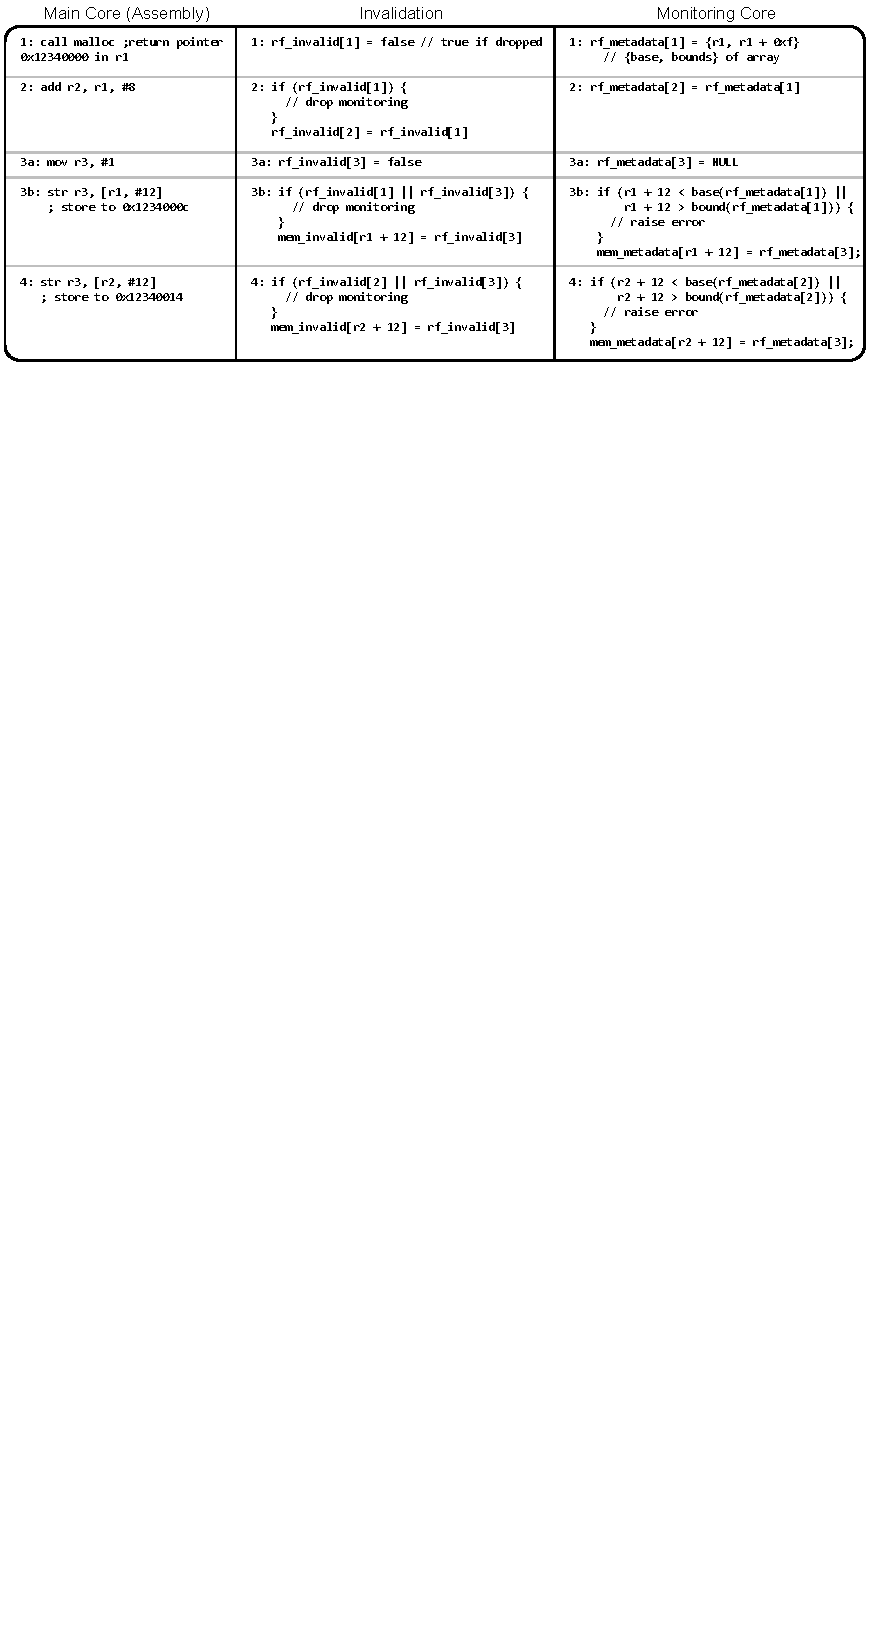
\includegraphics{monitoring_dift_drop/figs/example_invalid.pdf}
    \caption{Example of using invalidation information to prevent false positives.}
    \label{fig:monitoring_dift_drop.dropping.example_invalid}
  \end{center}
\end{figure}

The key cause of false positives is dropping monitoring operations that update
metadata. Dropping monitoring operations that check for an error (such as the
check for line 4 in
Figure~\ref{fig:monitoring_dift_drop.dropping.example_full}) can only cause
false negatives and will never cause false positives. On the other hand,
skipping monitoring operations that update metadata can lead to false positives
and false negatives.  Essentially, when an update operation is skipped, we can
no longer trust the corresponding metadata. Thus, our general approach for
preventing false positives is to associate a 1-bit invalidation flag with each
metadata in order to mark these metadata as valid or invalid, as was done for
the hard real-time monitoring architecture presented in
Chapter~\ref{chap:monitoring_hard_drop}. Furthermore, this
invalidation information is propagated in the same way that metadata is.
Figure~\ref{fig:monitoring_dift_drop.dropping.example_invalid} shows an example
of associating invalidation flags with metadata. Suppose that the monitoring
for line 1 is dropped in order to meet the overhead target. When a monitoring
event is dropped, metadata that would have been updated is marked as invalid.
In this case, instead of the normal operation of marking {\tt rf\_invalid[1]}
as {\tt false}, it is instead marked as {\tt true}. Thus, when line 3 is
reached, the monitoring event is dropped since {\tt rf\_invalid[1]} is marked
as true. Note that in this case, line 2 also propagates this invalidation flag
to {\tt rf\_invalid[2]} and causes the check performed on line 4 to also be
dropped. This is necessary because an error would have been raised even if the
access on line 4 was within bounds.

\subsection{Dataflow Engine for Preventing False Positives}
\label{sec:monitoring_dift_drop.dropping.arch}

% Dataflow engine high-level
\begin{figure}
  \begin{center}
    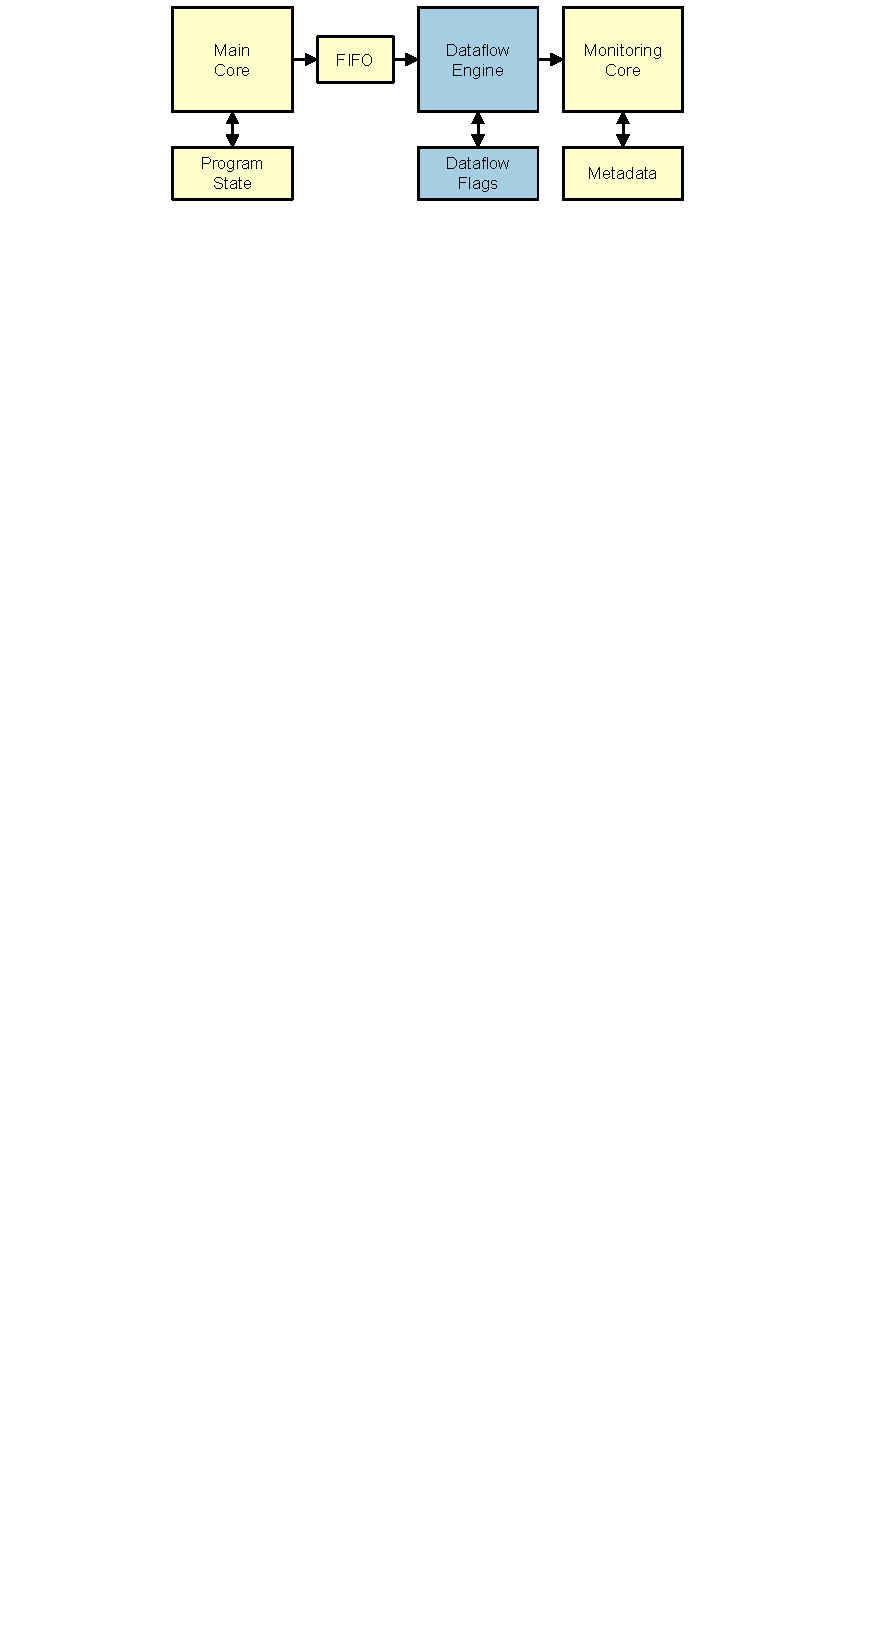
\includegraphics{monitoring_dift_drop/figs/dataflow_overview.pdf}
    \caption{Hardware support for dropping.}
    \label{fig:monitoring_dift_drop.dropping.dataflow_overview}
  \end{center}
\end{figure}

Although the functionality of dropping and invalidation could be implemented on
the monitor, this is unlikely to be much faster than performing the full
monitoring operations.  Instead, in order to efficiently support dropping
monitoring events and to prevent false positives, we propose to insert a
hardware module between the main core and monitor (see
Figure~\ref{fig:monitoring_dift_drop.dropping.dataflow_overview}).  This module
handles the invalidation operations shown in the middle column of
Figure~\ref{fig:monitoring_dift_drop.dropping.example_invalid}.  There are two
operations that are done for handling invalidation information:

\begin{enumerate}
  \item Propagate invalidation flags, following the dataflow of metadata.
  \item Filter out monitoring operations based on invalidation flags.
\end{enumerate}

% Detailed architecture of dataflow engine
\begin{figure}
  \begin{center}
    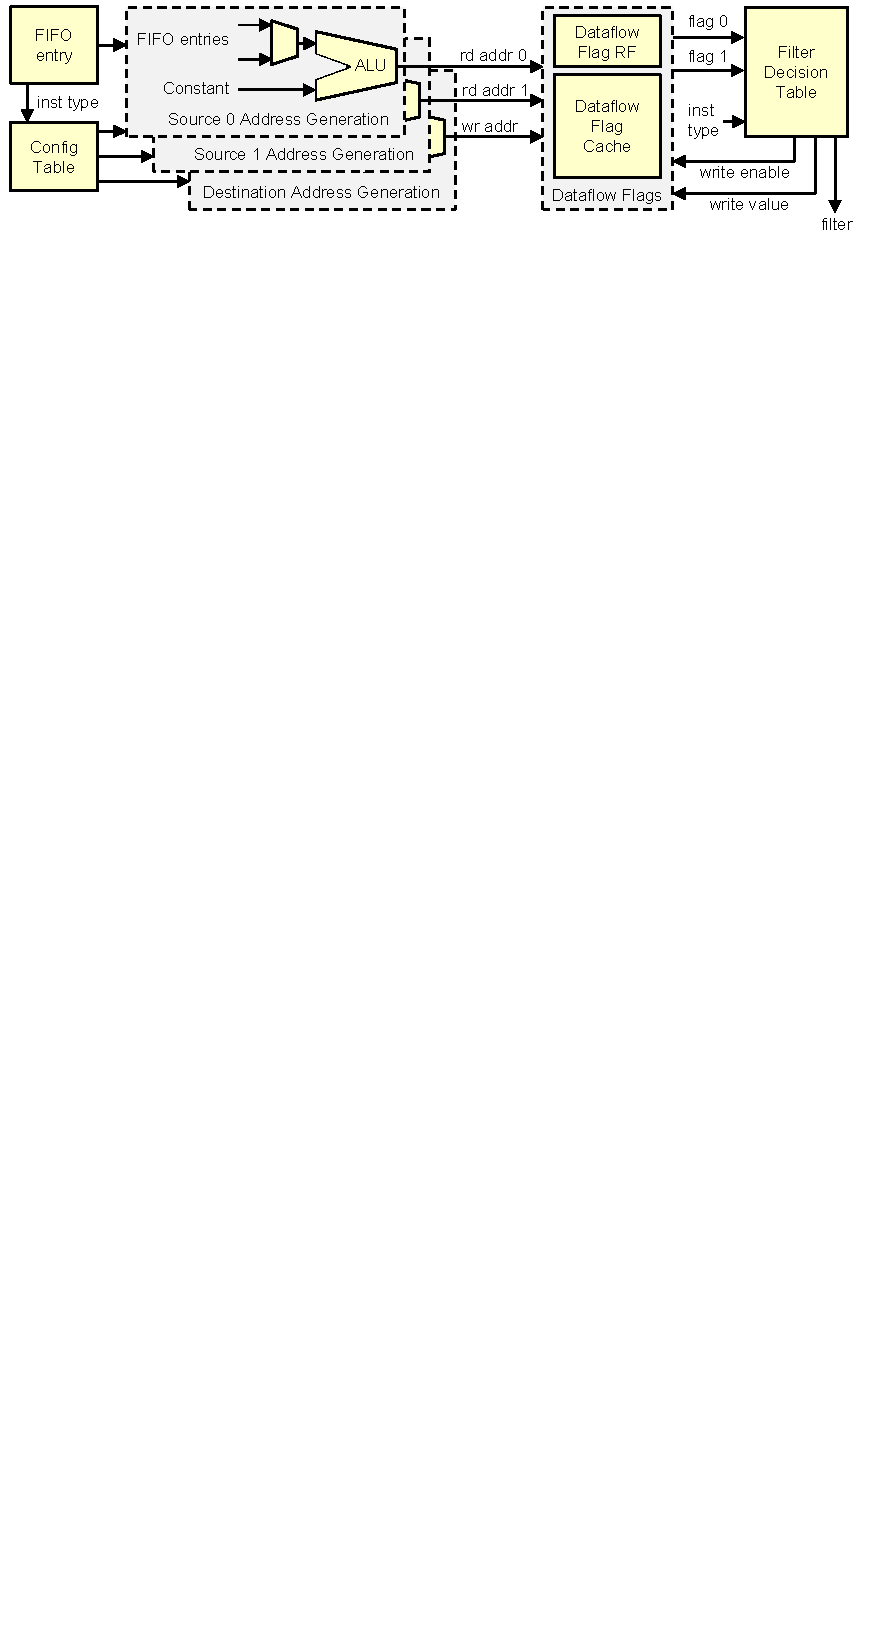
\includegraphics{monitoring_dift_drop/figs/dataflow_architecture.pdf}
    \caption{Hardware architecture of the dataflow engine.}
    \label{fig:monitoring_dift_drop.dropping.dataflow} 
  \end{center}
\end{figure}

Thus, the hardware acts effectively as a dataflow tracking engine in order to
track a 1-bit invalidation flag per metadata.
Figure~\ref{fig:monitoring_dift_drop.dropping.dataflow} shows a detailed block
diagram of this hardware module. The dataflow engine uses two address
generation units to read in up to two invalidation flags. These source
invalidation flags are used to decide whether a monitoring event should
filtered. A third address generation unit is used to optionally specify a
target to propagate the invalidation information. The module includes a
register file to store invalidation flags corresponding to register file
metadata. In addition, it uses a small memory-backed cache to handle
invalidation flags corresponding to memory metadata. The fact that the dataflow
flags are backed to memory differs from the design presented in
Chapter~\ref{chap:monitoring_hard_drop} for hard real-time systems. This allows
the architecture to have perfect invalidation information without aliasing. In
the worst-case, misses in the dataflow flag cache can cause high overheads for
dropping. However, we expect misses to be rare.

Since different monitoring operations are performed based on instruction type,
the dataflow engine is also configured based on instruction type. The source
and operation of the address generation units are set based on instruction
type. Note that the address generation units also take information from the
monitored event as inputs. Thus, in the same way that the monitor selects
metadata based on register indices or memory address of the specific monitoring
event, the dataflow engine also reads the appropriate flags. In addition, the
filter decision table is configured based on instruction type to decide what
combination of input flags will lead to a filtered event and whether
propagation is required.

\subsection{Filtering Null Metadata}
\label{sec:monitoring_dift_drop.dropping.null_filtering}

% Null filtering code example
\begin{figure}
  \begin{center}
    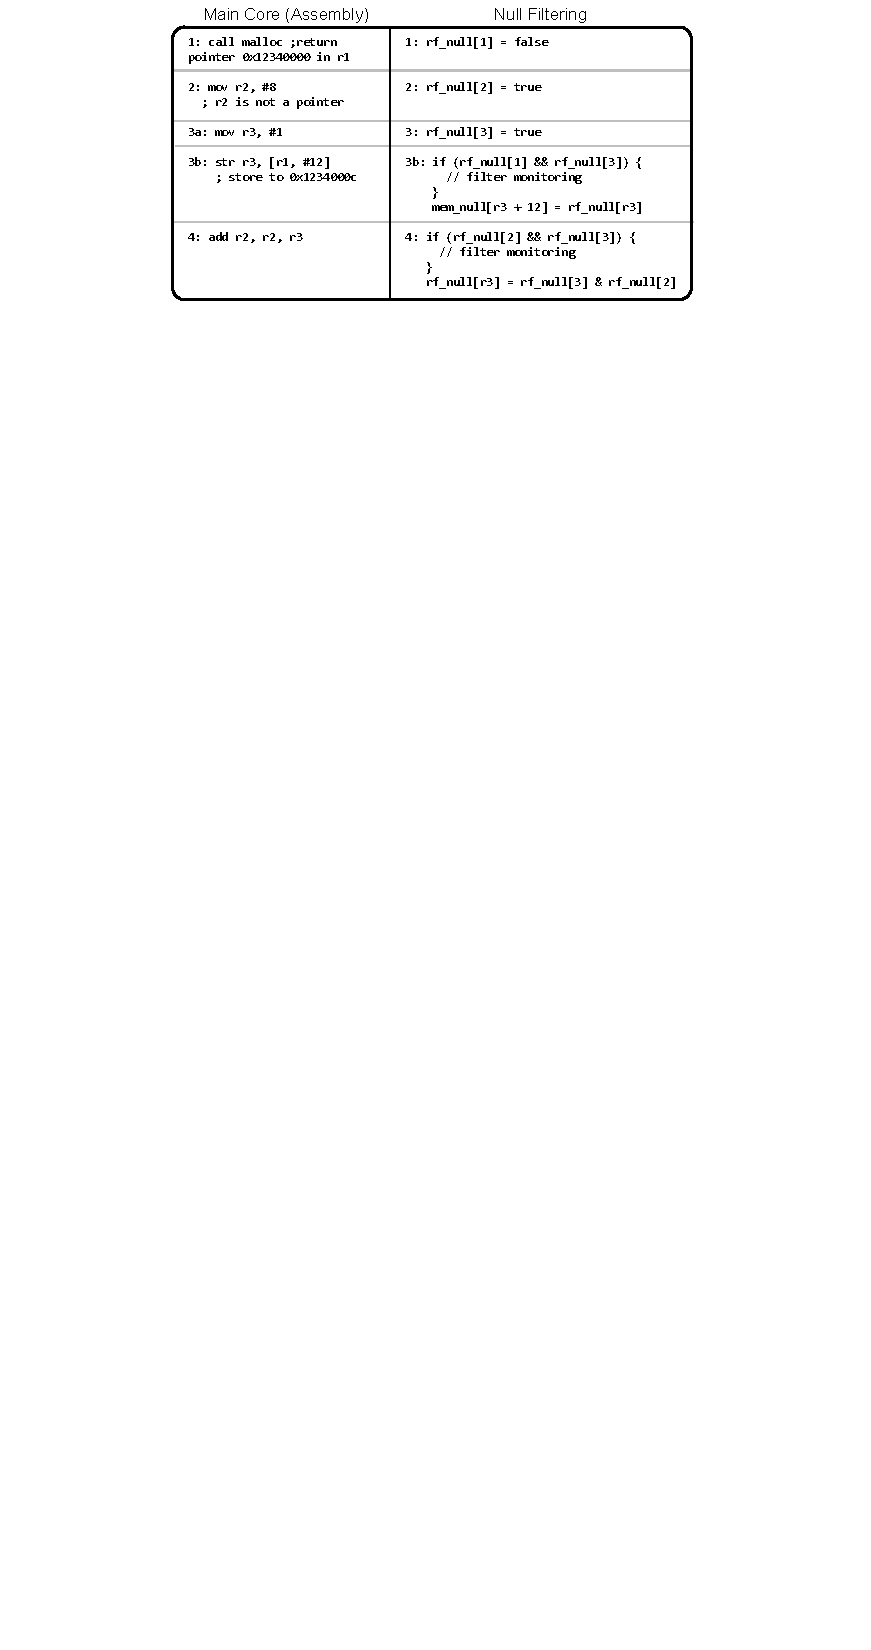
\includegraphics{monitoring_dift_drop/figs/example_null_filtering.pdf}
    \caption{Example of using information about null metadata to filter monitoring events.}
    \label{fig:monitoring_dift_drop.dropping.example_null} 
  \end{center}
\end{figure}

One way to reduce the number of monitoring events that must be handled by the
monitor is to filter out monitoring events that correspond to operating on null
metadata. Null metadata correspond to events that are not relevant to the
monitor. For example, Hardbound \cite{hardbound-asplos08} filters out
operations on non-pointer (i.e., no base and bounds metadata) instructions
since it is not relevant to array bounds checking. More recently, FADE
\cite{fade-hpca14} has been proposed as a general hardware module to perform
this null metadata filtering for a variety of monitoring schemes. Our
architecture is able to support this null metadata filtering with a small
modification.

Figure~\ref{fig:monitoring_dift_drop.dropping.example_null} shows an example of
how this null filtering operates.  Here, the main core's code has been slightly
modified from Figure~\ref{fig:monitoring_dift_drop.dropping.example_full} and
on line 2, {\tt r2} is no longer set as an array pointer.  Without null
metadata filtering, the instruction for line 4 would be forwarded to the
monitor since the system does not know whether {\tt r2} contains a pointer
address or not. However, if we use a 1-bit flag to mark {\tt r2} as null when
it is loaded with a constant, then we can propagate this null information and
filter out monitoring for line 4.

The operations performed by null filtering are almost identical to the
operations needed for invalidation shown in
Figure~\ref{fig:monitoring_dift_drop.dropping.example_invalid} except for a
small change in the propagation policy. Instead of taking a logical OR of the
source invalidation flags to determine whether monitoring can be skipped, null
metadata filtering takes a logical AND of the source null flags.  Thus, we can
easily enable this null metadata filtering on our architecture by extending the
dataflow flags to be two bits wide. One bit is used to keep track of
invalidation information while the second bit is used to keep track of null
information. All flags are initialized to null and the filter decision table is
extended with the propagation and filtering decision rules for null metadata
filtering.  The result is a single hardware design that enables both partial
monitoring and null metadata filtering.


%\section{Dropping Policies} 
\label{sec:monitoring_dift_drop.policies}

In order to use partial monitoring to enable adjustable overhead, we must also
specify a policy for when and which monitoring events are dropped. In this
section, we discuss some of the options and trade-offs for dropping policies.
We split this decision into two components: 
\begin{enumerate} 
  \item When do we need to drop events in order to enable reduced overhead? (Section~\ref{sec:monitoring_dift_drop.policies.when}) 
  \item Which events should be dropped? (Section~\ref{sec:monitoring_dift_drop.policies.which}) 
\end{enumerate}

\subsection{Deciding When to Drop} 
\label{sec:monitoring_dift_drop.policies.when}

% Slack
\begin{figure} 
  \begin{center}
    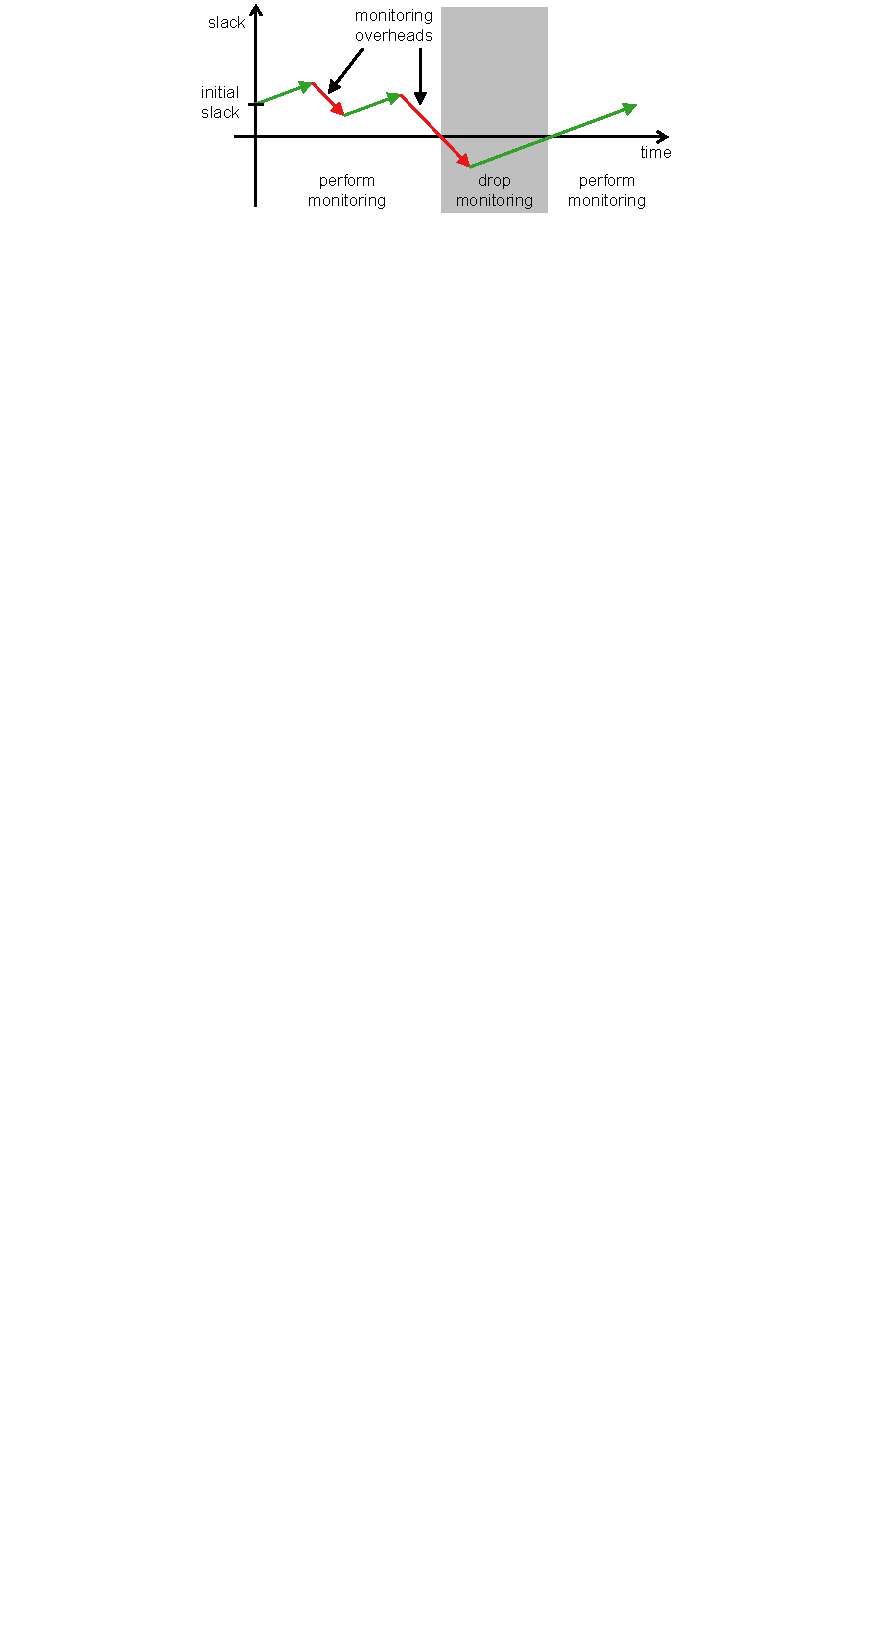
\includegraphics{monitoring_dift_drop/figs/slack.pdf} 
    \caption{Slack and its effect on monitoring over time.}
    \label{fig:monitoring_dift_drop.policies.slack} 
  \end{center} 
\end{figure}

In this section, we discuss two possible ways to determine when events should
be dropped.  The first possibility is to probabilistically drop events. By
setting the probability of dropping events appropriately, overhead can be
reduced. This works well for enabling partial monitoring for cooperative
testing and debugging since the randomness allows different users and runs to
monitor different portions of the program. However, using a probabilistic
dropping policy can make it difficult to meet a target overhead without prior
profiling.

Alternatively, we can specify a target overhead and estimate, at run-time, the
overhead of monitoring in order to decide whether dropping is needed.  The
overhead budget is specified as a percentage of the main program's execution
cycles without monitoring. In order to estimate the overhead at run-time, we
define \emph{slack} as the number of cycles of monitoring overhead that can be
incurred while staying within the budget target. Slack is essentially the
difference between the actual overhead seen and the budget specified. Slack is
generated as the main program runs and consumed as monitoring overheads occur.
For example, if no monitoring overheads occur during 1000 cycles of the main
program's execution and the designer sets a 20\% overhead target, then the
slack that is built up during this period is 200 cycles. If the main core is
then stalled for 50 cycles due to monitoring, then the remaining slack is 150
cycles.  In addition to this accumulated slack, a small amount of initial slack
can be given in order for monitoring to be performed at the start of a program.
Figure~\ref{fig:monitoring_dift_drop.policies.slack} shows an example of how
slack can change over time.  In this slack-based policy, if the slack falls
below zero (i.e., the overhead budget is exceeded), then monitoring events are
dropped.

Slack can be easily measured in hardware by using a counter that increments on
every $k$-th cycle of the main core (e.g., every 5th cycle for a 20\% target
budget). The value of this counter is the accumulated slack. Whenever the main
core is stalled due to the monitor, the measured slack is decremented. It is
difficult to precisely determine the entire impact of monitoring on the main
core due to the difficulty in measuring certain overheads such as contention
for shared memory. However, we have found that using only the stalls due to
FIFO back pressure works well in practice.

\subsection{Deciding Which Events to Drop} 
\label{sec:monitoring_dift_drop.policies.which}

\begin{figure} 
  \begin{center} 
    \begin{subfigure}[Unrestricted Dropping] {
      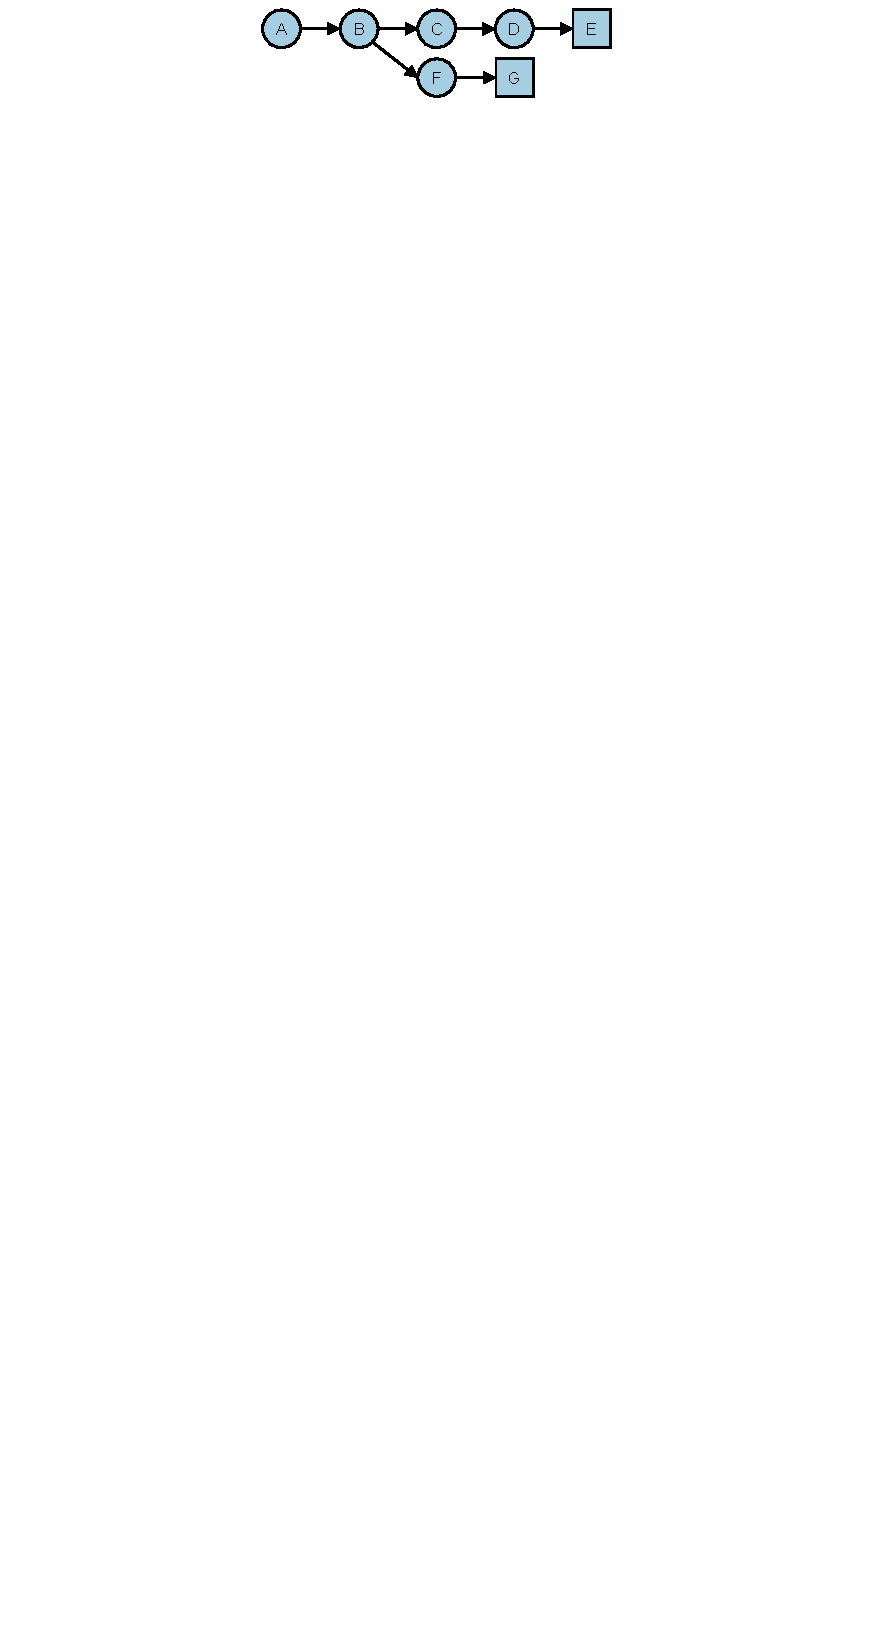
\includegraphics{monitoring_dift_drop/figs/unrestricted_drop.pdf}
      \label{fig:monitoring_dift_drop.policies.all_drop} 
    }
    \end{subfigure}
    \\
    \begin{subfigure}[Source-Only Dropping] { 
      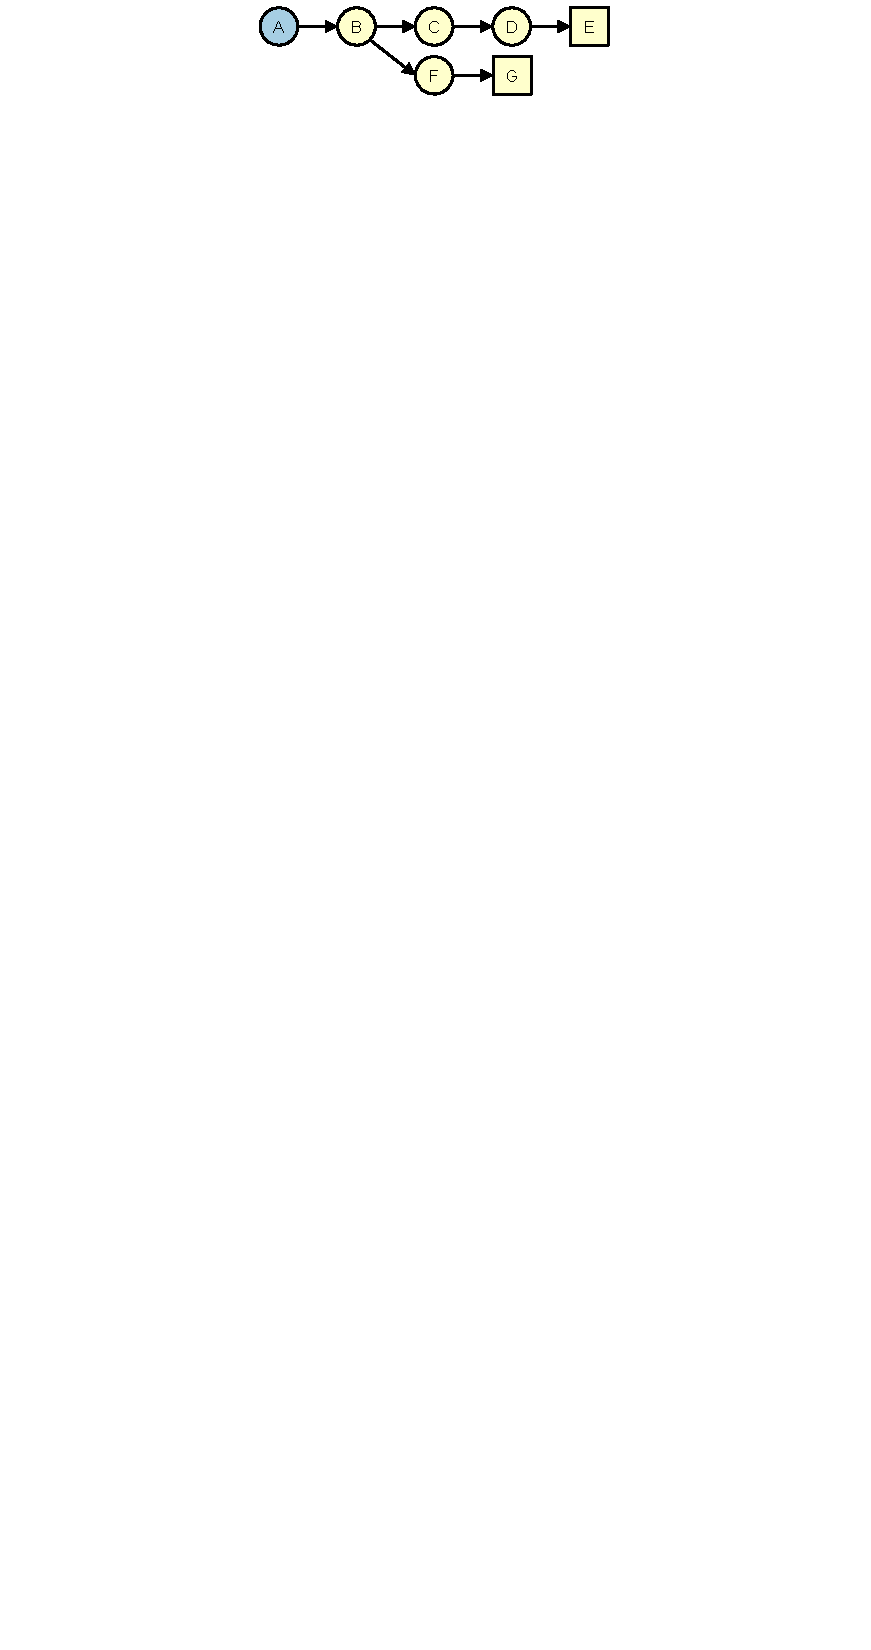
\includegraphics{monitoring_dift_drop/figs/source_drop.pdf}
      \label{fig:monitoring_dift_drop.policies.source_drop} 
    } 
    \end{subfigure}
    \\
    \begin{subfigure}[Sub-Flow Dropping] { 
      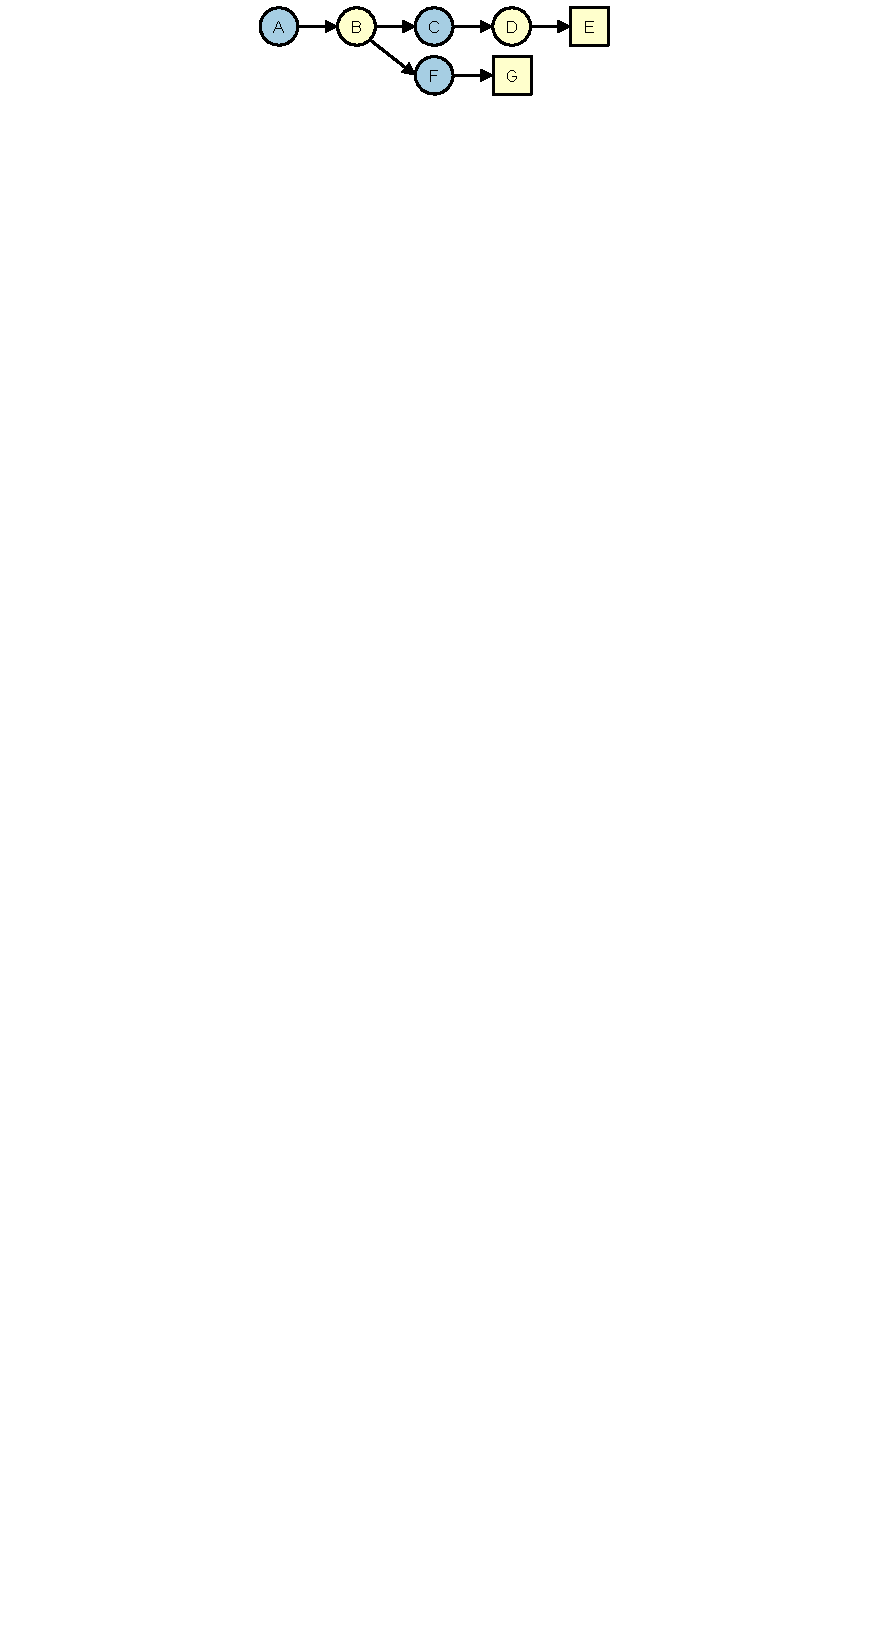
\includegraphics{monitoring_dift_drop/figs/subflow_drop.pdf}
      \label{fig:monitoring_dift_drop.policies.subflow_drop} 
    } 
    \end{subfigure}
  \end{center} 
  \caption{Comparison of dropping policies using metadata dependence graphs.
  Square nodes represent events where check are performed. Blue (dark) nodes
  indicate which nodes can be dropped.} 
  \label{fig:policies.policies} 
\end{figure}

In addition to deciding when dropping is required, trade-offs also exist in
deciding which events should be dropped.  The simplest policy is to drop
monitoring events when slack is less than or equal to zero.  However, this can
result in wasted work. For example, consider the metadata dependence graph
shown in Figure~\ref{fig:monitoring_dift_drop.policies.all_drop}. Here, an edge
from node {\tt A} to node {\tt B} represents that if event {\tt A} is dropped,
then due to its invalidated metadata, it will cause event {\tt B} to be
dropped. Square nodes indicate events where monitoring checks are performed. In
the example, suppose that event {\tt E} is meant to perform a check operation
but is dropped.  In this situation, the monitoring operations that were done
for events {\tt C} and {\tt D} were wasted since their results were not used
for any monitoring checks.  That is, by the time we decide to drop event {\tt
E}, we have already updated metadata for events {\tt C} and {\tt D} even though
they are no longer needed.

An alternative dropping policy which eliminates this wasted work is to only
make dropping decisions at the root or source of these metadata flows (see
Figure~\ref{fig:monitoring_dift_drop.policies.source_drop}). That is, we will
decide to either monitor or not monitor an entire metadata flow. An example of
these source nodes is the monitoring done to initialize base and bounds
information on {\tt malloc} for an array bounds check. These source nodes are
easily identifiable by the dropping hardware because they typically correspond
to the special instructions that are used to set up metadata information. Thus,
it is not necessary to generate and analyze the monitoring dependence graph to
identify source nodes. We refer to this dropping decision policy as
\emph{source-only dropping} and we refer to the previous policy of dropping any
event as \emph{unrestricted dropping}.

More complex dropping policies can be implemented given more detailed
information about the monitoring dependence graph. This information can be
found through static analysis or profiling, though we do not explore how to
find it in detail here. Given this information, we describe one possible policy
to use it, which we call \emph{sub-flow dropping}. Sub-flow dropping makes
dropping decisions at a granularity in between unrestricted dropping and
source-only dropping (see
Figure~\ref{fig:monitoring_dift_drop.policies.subflow_drop}).  The basic idea
of sub-flow dropping is to drop portions of the monitoring dependence graph at
the smallest granularity such that no work is wasted.  Sub-flow dropping allows
source nodes to be dropped and nodes after branch points in the monitoring
dependence graph to be dropped. From
Figure~\ref{fig:monitoring_dift_drop.policies.subflow_drop}, this corresponds
to nodes {\tt A}, {\tt C}, and {\tt F}. For example, dropping node {\tt C}
causes nodes {\tt D} and {\tt E} to be skipped. However, performing monitoring
on the remaining nodes allows the check at node {\tt G} to be performed with no
wasted work.  Similarly, dropping {\tt F} allows node {\tt E} to be checked
with no wasted work.  Note that sub-flow dropping can still result in wasted
work if there are merge points in the monitoring dependence graph and only part
of the incoming flows are dropped, but it should result in less wasted work
than compared to an unrestricted dropping policy. 

Source-only dropping will result in no wasted work and thus better coverage at
a given overhead than unrestricted dropping. However, because of the
coarser-grained decision, it may be more difficult to closely match overhead
targets.  Sub-flow dropping enables a design point in between unrestricted
dropping and source-only dropping in terms of matching overhead and coverage
achieved.  If the monitoring dependence graph is highly connected, then
source-only dropping will perform poorly. On the other hand, we expect
source-only dropping to work well when there are a large number of independent
metadata flows.  Monitoring dependence graphs with a large number of branches
will favor a sub-flow dropping policy.

The choice of dropping policy can also depend on whether probabilistic dropping
is performed instead of slack-based dropping.  Probabilistic dropping works
poorly with an unrestricted dropping policy. Since every event in a dependent
chain (e.g., events {\tt A} through {\tt E}) needs to be monitored in order for
the monitoring check to be useful, randomly dropping any event is likely to
cause the final check to be invalid by dropping at least one event in the
chain. Instead, source-only dropping works well when performing probabilistic
dropping.

Depending on the target application of partial monitoring, different policies
are more applicable.  For applications where closely matching an overhead
target is important, a slack-based, unrestricted dropping policy is
appropriate. However, if matching the overhead target is not as important, then
a slack-based, sub-flow or source-only dropping policy could provide better
coverage.  Finally, if the goal is to use partial monitoring to enable
cooperative debugging and testing with very low overhead, then a probabilistic,
source-only or sub-flow dropping policy can be used to provide good total
coverage over multiple runs.


%\section{Evaluation}
\label{sec:monitoring_dift_drop.evaluation}

\subsection{Experimental Setup}
\label{sec:monitoring_dift_drop.evaluation.setup}

We implemented our dataflow-guided monitoring architecture by modifying the ARM
version of the gem5 simulator \cite{gem5} to support parallel run-time
monitoring. We implement the monitor as a software-based monitor running on a
parallel processor core, similar to LBA \cite{lba-asid06}.  We model the main
and monitoring cores as running at 2.5 GHz with 4-way set-associative 32 kB
private L1 I/D caches and a shared 8-way 2 MB L2 cache. This setup is similar
to the Snapdragon 801 processor commonly found in mobile systems. A 16-entry
FIFO was used to connect the main core to the monitoring core. The dataflow
engine uses a 1 kB cache for invalidation and null flags.

In order to explore the generality of the architecture for different monitors,
we implemented five different monitors: uninitialized memory check (UMC), array
bounds check (BC), dynamic information flow tracking (DIFT), instruction-mix
profiling (IMP), and LockSet-based race detection (LS).  Since we implement the
monitor using a processor core and our dataflow engine was designed to be
generally applicable, the same hardware platform supports all of these
monitoring techniques.  Uninitialized memory check seeks to detect loading from
memory locations that are not initialized first. Array bounds check is a monitoring
scheme that aims to detect buffer overflows where memory accesses go beyond the
boundaries of an array. We modify the implementation of {\tt malloc} to set
base and bound metadata information. Dynamic information flow tracking is a
security monitoring scheme which detects when information from untrusted
sources is used to affect the program control flow (i.e., indirect control
instructions). For the benchmarks we consider, we mark data read from files as
untrusted. We implemented a multi-bit DIFT scheme which marks untrusted data
with a 32-bit metadata identifier so that if an error is detected, it is
possible to have information about where the data originated from.
Instruction-mix profiling counts the number of ALU, load, store, and control
instructions that are executed. This profiling information can be useful for
performing optimizations or to detect malicious software \cite{tang-raid14}.
Finally, LockSet \cite{eraser-tocs97} attempts to detect possible race conditions in
multi-threaded programs by tracking metadata about which locks are protecting
shared memory locations. If a shared memory location is accessed while
unprotected then a race condition may exist.

We tested our system using benchmarks from SPECint CPU2006 \cite{spec2006}.
Since our implementation of BC depends on the modification of {\tt malloc} to
set array bounds information, we focus on the C SPECint benchmarks. Although we
do not show results for the C++ benchmarks, we note that the results for UMC,
DIFT, and IMP for these benchmarks are similar to the other results shown.  We
fast-forwarded each benchmark for 1 billion instructions and then simulated for
2 billion instructions. 

Since LockSet race detection requires multi-threaded programs, we tested it
using the applications from the SPLASH-2 benchmark set \cite{splash-isca95}.
Each benchmark was run using 2 main cores to run the benchmark application.
{\tt fmm} and {\tt raytrace} were run without fast-forwarding because they ran
to completion in under 2 billion instructions.  Each main core was connected to
a dataflow engine and a monitoring core.

\subsection{Baseline Monitoring Overhead}

% Filter monitoring overheads
\begin{figure}
  \begin{center}
    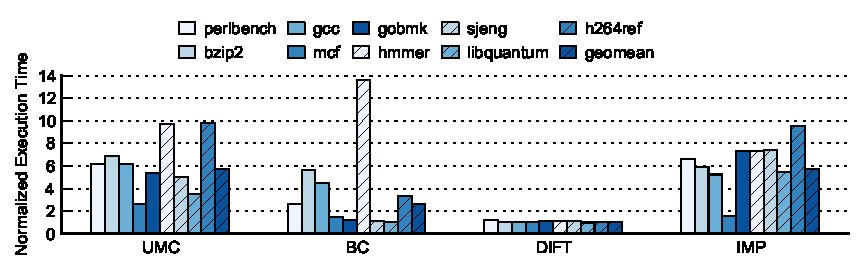
\includegraphics{monitoring_dift_drop/data/filter_mon.pdf}
    \caption{Monitoring overhead with null metadata filtering.}
    \label{fig:monitoring_dift_drop.evaluation.filter_mon}
  \end{center}
\end{figure}

Figure~\ref{fig:monitoring_dift_drop.evaluation.filter_mon} shows the execution
times of performing monitoring with null filtering enabled normalized to the
execution time of the benchmarks without monitoring. UMC sees normalized
execution times of 2.6-9.8x with an average of 5.7x.  For BC, normalized
execution times are 2.7x on average and range from 1.02x to 13.6x.  DIFT sees
an average of 1.1x slowdown with a maximum slowdown of 1.3x with null metadata
filtering. This low overhead is due to the fact that for our implementation of
DIFT on SPEC benchmarks, we only mark data read from files as tainted. Instead,
if we targeted network or streaming applications, which have larger amounts of
untrusted input data, we would observe higher overhead. IMP shows normalized
execution times of 1.6-9.5x with an average of 5.8x. Overheads for LS (not
pictured) applied to the SPLASH-2 benchmarks are 1.04-1.29x after null metadata
filtering and the average overhead observed is 1.13x.  Our baseline system and
overheads are similar to previous multi-core monitoring systems such as
LBA-accelerated \cite{lba-isca08} and FADE \cite{fade-hpca14} (see
Table~\ref{tab:monitoring_dift_drop.monitoring.previous_overheads}). In
Section~\ref{sec:monitoring_dift_drop.evaluation.fpga}, we also evaluate a
higher performance, FPGA-based monitor that shows low tens of percent of
overhead. 

\subsection{Coverage with Adjustable Partial Monitoring}

% BC sweep
\begin{figure}
  \begin{center}
    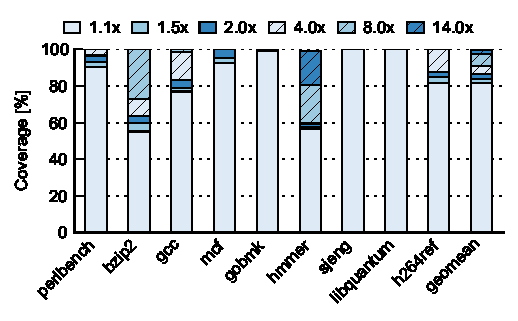
\includegraphics{monitoring_dift_drop/data/hb_sweep.pdf}
    \caption{Coverage vs. varying overhead budget for BC.}
    \label{fig:monitoring_dift_drop.evaluation.bc_sweep}
  \end{center}
\end{figure}

% UMC sweep
\begin{figure}
  \begin{center}
    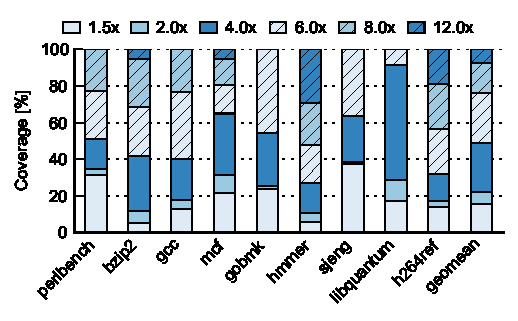
\includegraphics{monitoring_dift_drop/data/umc_sweep.pdf}
    \caption{Coverage vs. varying overhead budget for UMC.}
    \label{fig:monitoring_dift_drop.evaluation.umc_sweep}
  \end{center}
\end{figure}

% LS sweep
\begin{figure}
  \begin{center}
    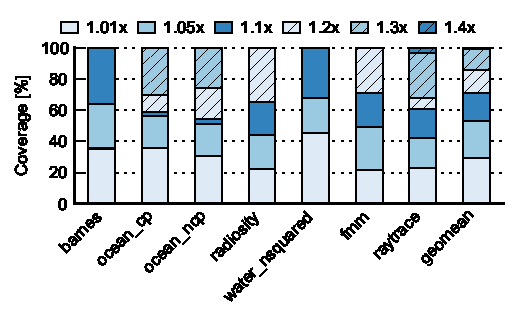
\includegraphics{monitoring_dift_drop/data/ls_sweep.pdf}
    \caption{Coverage vs. varying overhead budget for LS.}
    \label{fig:monitoring_dift_drop.evaluation.ls_sweep}
  \end{center}
\end{figure}

% IMP sweep
\begin{figure}
  \begin{center}
    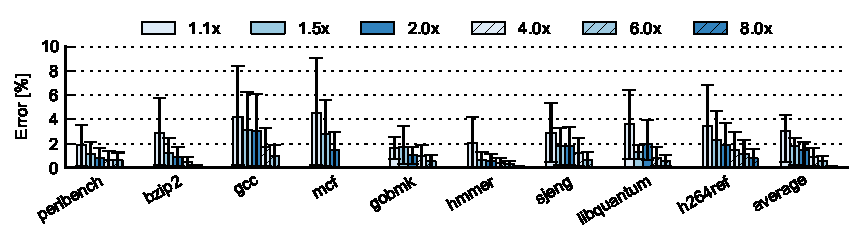
\includegraphics{monitoring_dift_drop/data/imp_sweep.pdf}
    \caption{Average error vs. varying overhead budget for instruction-mix
    profiling. Whisker bars show min and max errors.}
    \label{fig:monitoring_dift_drop.evaluation.imp_sweep}
  \end{center}
\end{figure}

In this section, we evaluate the effectiveness of using partial monitoring to
trade-off coverage for reduced overhead.  For these results, we use a
slack-based, unrestricted dropping policy.
Figure~\ref{fig:monitoring_dift_drop.evaluation.bc_sweep} shows the monitoring
coverage achieved by array bounds checking as we vary the overhead budget.  We
define \emph{monitoring coverage} as the percentage of dynamic checks that are
performed (indirect jumps in DIFT, loads in UMC, and memory accesses in BC and
LS).  The metric is chosen to understand how likely an error/attack instance is
to be detected on an individual system, assuming that errors/attacks are
uniformly distributed across checks. This may not necessarily be true for
actual errors/attacks and so the reported coverage may not be the same as the
probability of detecting actual errors/attacks.  However, we believe this
metric provides a good initial estimate of the detection capabilities of the
system.  In the figure, the bottom portion of each bar shows the coverage for a
1.1x overhead target and the additional coverage for increased overhead targets
are stacked above this.

We see that by varying the overhead budget, the coverage achieved also varies.
With only a 1.1x overhead target, array bounds check still achieves over 80\%
monitoring coverage on average. The high coverage achieved with such low
overhead is due to two main effects.  The first is that monitoring can be done
in parallel, providing a certain level of monitoring coverage without
introducing overhead. The second effect is that there may still exist a large
number of monitoring events that do not lead to bounds checks. As a result,
dropping these events can reduce overhead without a large impact on monitoring
coverage.

Figure~\ref{fig:monitoring_dift_drop.evaluation.umc_sweep} shows the analogous
graph for UMC. Again we see that varying overhead budgets enables partial
monitoring.  With a 2x overhead target, UMC achieves 22\% monitoring coverage
on average and with a 4x overhead target, this increases to 49\%.  Even higher
coverage can be achieved by allowing higher overhead budgets.  Similarly,
Figure~\ref{fig:monitoring_dift_drop.evaluation.ls_sweep} shows the coverage
achieved by LS.  With only a 1.01x overhead, LS achieves 30\% coverage on
average. This increases to 71\% coverage with a 1.1x overhead budget.  For DIFT
(not pictured), an overhead target of 1.05x is enough for all benchmarks tested
to reach 100\% coverage.  Note that the overheads shown are the target
overhead. In some cases, a high overhead target is needed in order to achieve
100\% coverage. For example, for {\tt mcf} with UMC monitoring, a 12x overhead
target is needed to achieve 100\% coverage while the overheads of performing
monitoring in full were 2.6x (see
Figure~\ref{fig:monitoring_dift_drop.evaluation.filter_mon}). This is due to
the fact that we accumulate slack gradually and so bursty monitoring events may
require a higher overhead target in order for all monitoring to be performed.
However, the actual overheads seen are in-line with the overhead of performing
monitoring without dropping (e.g., {\tt mcf} with UMC monitoring at a 12x
overhead target shows a 2.6x overhead).

The instruction-mix profiling monitor does not perform check operations. Thus,
the concept of coverage is not applicable here. Instead, for each instruction
type profiled, we calculate its count as a percentage of the total instructions
monitored. We take the difference of these percentages compared to the case
when full monitoring is performed to calculate the error.
Figure~\ref{fig:monitoring_dift_drop.evaluation.imp_sweep} shows the min, max,
and average error across instruction types for each benchmark and for varying
overhead. We see that with a 1.1x overhead, a max error of 9\% is observed
across the benchmarks and the average error across instruction types and
benchmarks is 3\%. 

\subsection{FPGA-based Monitor}
\label{sec:monitoring_dift_drop.evaluation.fpga}

% Flex UMC sweep
\begin{figure}
  \begin{center}
    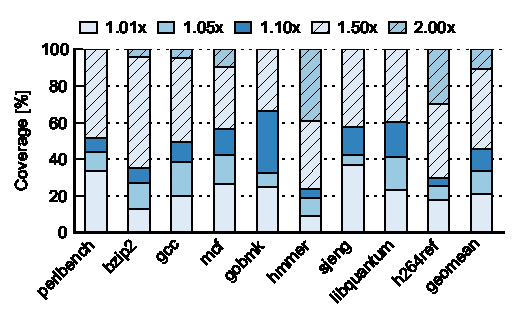
\includegraphics{monitoring_dift_drop/data/fpga_umc_sweep.pdf}
    \caption{Coverage versus varying overhead budget for UMC running on an FPGA-based monitor.}
    \label{fig:monitoring_dift_drop.evaluation.fpga_umc_sweep}
  \end{center}
\end{figure}

In addition to evaluating our system for a core-based monitor, we also
evaluated partial monitoring on a higher performance FPGA-based monitor. This
setup is based on the FlexCore \cite{flexcore-micro10} setup and uses a
fully-pipelined monitor running on an FPGA fabric at half the frequency of the
main core. In this case, the full overheads of monitoring
range from 1.1-1.9x with an average overhead of 1.4x.
Figure~\ref{fig:monitoring_dift_drop.evaluation.fpga_umc_sweep} shows the
coverage achieved as we sweep the overhead target from 1.01-2.0x. We see that
partial monitoring can allow the overhead of such a system to be pushed to 1.1x
while still providing 45\% coverage.

\subsection{Comparing Dropping Policies}

\begin{figure}
  \begin{center}
  \begin{subfigure}[Overhead budget error.]{
    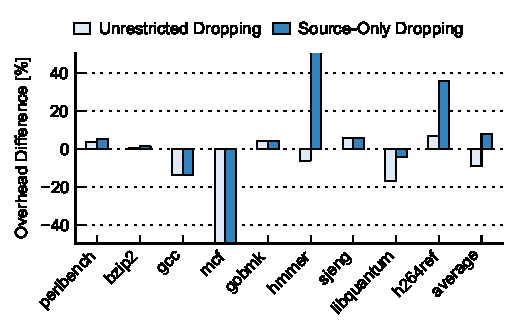
\includegraphics{monitoring_dift_drop/data/umc_overhead.pdf}
    \label{fig:monitoring_dift_drop.evaluation.umc_exec_time}
  }
  \end{subfigure}
  \\
  \begin{subfigure}[Coverage.]{
    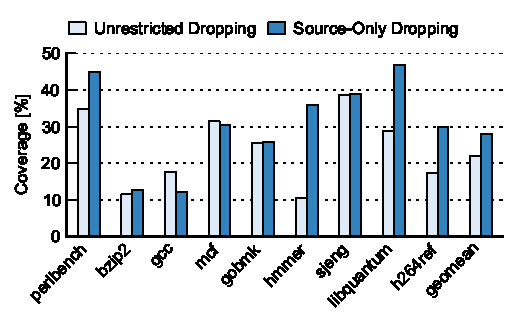
\includegraphics{monitoring_dift_drop/data/umc_coverage.pdf}
    \label{fig:monitoring_dift_drop.evaluation.umc_coverage}
  }
  \end{subfigure}
  \caption{Comparing dropping policies for UMC.}
  \label{fig:monitoring_dift_drop.evaluation.umc_policies}
  \end{center}
\end{figure}

In this section, we evaluate the trade-offs between different dropping
policies.  Figure~\ref{fig:monitoring_dift_drop.evaluation.umc_exec_time} shows
the difference between the overhead budget and the run-time monitoring overhead
for UMC when the overhead target is set to 2.0x. A positive value means that
the overhead target was overshot while a negative value indicates that the
overhead budget was met. For most benchmarks, we see similar results for
unrestricted dropping and source-only dropping due to the fact that UMC
consists of a large number of short, independent monitoring dependence chains.
Source-only dropping causes overshoot of the overhead target for {\tt hmmer}
and {\tt h264ref}.
Figure~\ref{fig:monitoring_dift_drop.evaluation.umc_coverage} shows the
coverage of UMC for unrestricted dropping and source-only dropping. We see
that, in several cases, source-only dropping achieves higher coverage than
unrestricted dropping while still closely matching the overhead target. For
example, {\tt perlbench} shows a 10\% increase in coverage and {\tt libquantum}
shows an 18\% increase in coverage by using source-only dropping. This is due
to the fact that some of the overhead of monitoring for unrestricted dropping
is being spent on wasted work as discussed in
Section~\ref{sec:monitoring_dift_drop.policies.which}.

\begin{figure}
  \begin{center}
  \begin{subfigure}[Overhead budget error.]{
    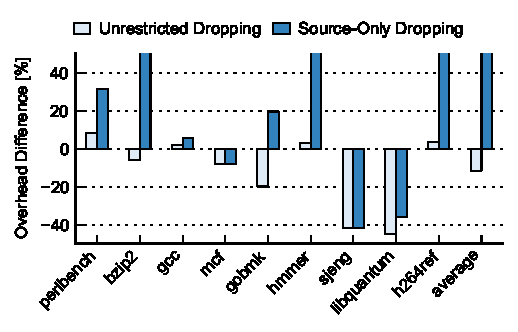
\includegraphics{monitoring_dift_drop/data/hb_overhead.pdf}
    \label{fig:monitoring_dift_drop.evaluation.bc_exec_time}
  }
  \end{subfigure}
  \\
  \begin{subfigure}[Coverage.]{
    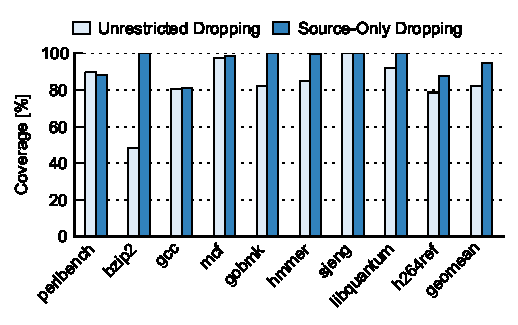
\includegraphics{monitoring_dift_drop/data/hb_coverage.pdf}
    \label{fig:monitoring_dift_drop.evaluation.bc_coverage}
  }
  \end{subfigure}
  \caption{Comparing dropping policies for BC.}
  \label{fig:monitoring_dift_drop.evaluation.bc_policies}
  \end{center}
\end{figure}

Next, we evaluate these trade-offs between source-only dropping and
unrestricted dropping for BC.
Figure~\ref{fig:monitoring_dift_drop.evaluation.bc_exec_time} shows the
overhead differences for BC and
Figure~\ref{fig:monitoring_dift_drop.evaluation.bc_coverage} shows the coverage
for BC.  Here, the overhead target is 1.5x.  From
Figure~\ref{fig:monitoring_dift_drop.evaluation.bc_exec_time}, we see that for
several benchmarks, source-only dropping fails to meet the specified overhead
target.  The overshoot of the overhead target is quite high with overhead
differences over 100\% for {\tt bzip2}, {\tt hmmer}, and {\tt h264ref}.  Since
only infrequently occurring array allocations are considered as source events
for BC, it can be difficult for source-only dropping to match overhead targets.
Although Figure~\ref{fig:monitoring_dift_drop.evaluation.bc_coverage} shows
higher coverage for source-only dropping, this is largely due to the fact that
it is running with higher overhead.
On the other hand, UMC showed higher coverage while matching overhead well with
source-only dropping because UMC monitoring consists of a large number of short,
independent dependences (i.e, store to load dependence).

From these results, we see that depending on the monitor and the program
behavior, source-only dropping can provide better coverage than unrestricted
dropping with the same overhead. However, unrestricted dropping is better at
meeting an overhead target.  Thus, for applications where staying within an
overhead target is especially important, such as soft real-time systems, a
slack-based, unrestricted dropping policy is more appropriate. On the other
hand, if maximum coverage is desired and occasional slowdowns are acceptable,
then source-only dropping can provide better coverage on average.

The results for the sub-flow dropping policy are not included in these graphs
because our profiling infrastructure to identify sub-flow nodes currently does
not support fast-forwarding. Instead, we compared the sub-flow dropping with
other policies by running simulations for 1 billion instructions without
fast-forwarding. The results (not shown) showed that sub-flow dropping produced
similar coverage and overhead target matching to unrestricted dropping for the
benchmarks and monitors that we tested.

\subsection{Multiple-Run Coverage}

% Multi-run coverage with unrestricted dropping
\begin{figure}
  \begin{center}
    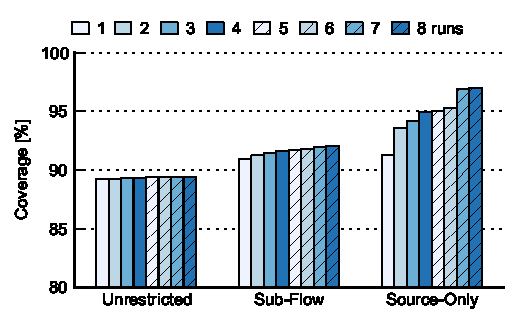
\includegraphics{monitoring_dift_drop/data/multi_run.pdf}
    \caption{Coverage over multiple runs for BC with a 10\% probability to not drop events.}
    \label{fig:monitoring_dift_drop.evaluation.multirun}
  \end{center}
\end{figure}

One application of partial monitoring with low overhead is to enable
cooperative debugging.  The idea with cooperative debugging is to use partial
monitoring with very low overhead across a large number of users or runs. By
varying the pattern of partial monitoring done on each run, the goal is to
achieve high coverage across multiple runs. Varying the monitoring that is done
for different runs can be achieved by using a probabilistic dropping policy.
Figure~\ref{fig:monitoring_dift_drop.evaluation.multirun} shows the total
coverage achieved over multiple runs for array bounds check using unrestricted,
sub-flow, and source-only dropping policies with probabilistic dropping.  These
numbers are averaged across all benchmarks. Here, we use a 10\% probability
that events are not dropped.  Each run was simulated for 500 million
instructions.  Since the effectiveness of cooperative debugging is often
measured by code coverage, coverage here is measured as the percentage of
static instructions which are monitored in at least one of the runs.  We see
that for the unrestricted dropping policy there is almost no increase in
coverage.  This is due to the fact that it is likely that at least one
monitoring event in a metadata dependence chain will be dropped with the
unrestricted dropping policy.  Instead, sub-flow dropping and source-only
dropping are much better suited for achieving high coverage over multiple runs.
Source-only dropping shows a 6\% increase in coverage with only eight runs
while sub-flow dropping shows a 1\% increase in coverage over eight runs.
While sub-flow dropping shows a slower increase in coverage than source-only
dropping, sub-flow dropping is better able to meet overhead targets.  With
enough runs, both sub-flow dropping and source-only dropping should be able to
reach 100\% code coverage.

\subsection{Area and Power Overheads}

% Area and Power Overheads
\begin{table}[tb]
  \begin{center}
    \begin{footnotesize}
    
% Full monitoring at zero slack

\begin{tabular}{|c|c|c|}
\hline

{\bf Monitor} & {\bf Peak Power [mW]} & {\bf Runtime Power [mW]} \\ \hline\hline

UMC  & 48 (4.9\%) & 29 (7.7\%) \\ \hline
BC   & 69 (7.1\%) & 41 (10.7\%) \\ \hline
DIFT & 72 (7.4\%) & 41 (10.6\%) \\ \hline
IMP  & 41 (4.3\%) & 20 (5.1\%) \\ \hline
LS   & 31 (3.2\%) & 13 (3.9\%) \\ \hline

\end{tabular}

    \end{footnotesize}
    \caption{Average power overhead for dropping hardware. Percentages 
    are normalized to the main core power.}
    \label{tab:monitoring_dift_drop.evaluation.area_power}
  \end{center}
\end{table}

Adding the dataflow engine in order to enable filtering and partial monitoring
adds overheads in terms of area and power consumption. We use McPat
\cite{mcpat-micro09} to get a first-order estimate of these area and power
overheads in a 40 nm technology node. McPat estimates the main core area as
2.71 mm$^2$ and the peak power usage as 965 mW averaged across all benchmarks.
The average runtime power usage was 385 mW. These area and power numbers
consist of the core and L1 cache, but do not include L2 cache, memory
controller, and other peripherals. The power numbers include dynamic as well as
static (leakage) power. For the dataflow engine, we modeled the ALUs used for
address calculation, the dataflow flag register file and cache, the
configuration tables, and the filter decision table. These were modeled using
the corresponding memory and ALU objects in McPat. We note that this is only a
rough area and power estimate since components such as the wires connecting
these modules have not been modeled. However, this gives a sense of the
order-of-magnitude overheads involved with implementing our approach.

Our results show that an additional 0.197 mm$^2$ of silicon area is needed, an
increase of 7\% of the main core area.
Table~\ref{tab:monitoring_dift_drop.evaluation.area_power} shows the peak and
runtime power overheads averaged across all benchmarks running with a 1.5x
monitoring overhead target. The peak power is 31-72 mW, which is less than 8\%
of the main core's peak power usage. Similarly, the average runtime power is
13-43 mW, corresponding to 4-11\% of the main core's runtime power.

% Runtime power of monitoring core
\begin{table}[tb]
  \begin{center}
    \begin{footnotesize}
    
% Runtime power for monitoring core

\begin{tabular}{|c|c|c|}
\hline

{\bf Monitor} & {\bf 1.5x Overhead} & {\bf Full Monitoring} \\ \hline\hline

UMC  & 338 mW & 363 mW \\ \hline
BC   & 320 mW & 343 mW \\ \hline
DIFT & 304 mW & 304 mW \\ \hline
IMP  & 345 mW & 367 mW \\ \hline
LS   & 327 mW & 327 mW \\ \hline

\end{tabular}

    \end{footnotesize}
    \caption{Average runtime power of the monitoring core.}
    \label{tab:monitoring_dift_drop.evaluation.monitor_power}
  \end{center}
\end{table}

Table~\ref{tab:monitoring_dift_drop.evaluation.monitor_power} shows the runtime
power usage of the monitoring core averaged across all benchmarks. These
results are shown for an overhead target of 1.5x as well as when full
monitoring is performed.



\chapter{DVFS Control for Soft Real-Time Systems}
\label{chap:exec_time_prediction}

\section{Introduction}
\label{sec:exec_time_prediction.introduction}

Many modern applications on mobile and desktop systems are interactive.
That is, users will provide inputs and expect a response in a timely manner.
For example, games must read in user input, update game state, and display the
result within a small time window in order for the game to feel responsive.
Previous studies on human-computer interaction have shown that latencies of 100
milliseconds are required in order to maintain a good experience
\cite{endo-osdi96, card-chi91, miller-afips68} while variations in response
time faster than 50 milliseconds are imperceptible \cite{lindgaard-bit06,
eqos-hpca15}. These tasks are effectively soft real-time tasks which have a
user response-time deadline. The task must finish by the deadline for good user
experience, but finishing faster does not necessarily improve the user
experience due to the limits of human perception.

As finishing these tasks faster is not beneficial, we can use power-performance
trade-off techniques, such as dynamic voltage and frequency scaling (DVFS), in
order to reduce energy usage while maintaining the same utility to the user. By
reducing the voltage and frequency, we can run the task slower and with less
energy usage. As long as the task still completes by the deadline, then the
experience for the user remains the same. 

Existing Linux power governors \cite{linux_governors} do not take into account
these response-time requirements when adjusting DVFS levels. More recent work
has looked at using DVFS to minimize energy in the presence of deadlines.
However, these approaches are typically reactive, using past histories of task
execution time as an estimate of future execution times \cite{gu-dac08,
choi-iccad02, pegasus-isca14, nachiappan-hpca15}.  However, the execution time
of a task can vary greatly depending on its input.  Reactive controllers cannot
respond fast enough to input-dependent execution time variations.  Instead,
proactive or predictive control is needed in order to adjust the operating
point of a task before it runs, depending on the task inputs. This has been
explored for specific applications \cite{gu-rtas08, zhu-hpca13, eqos-hpca15,
adrenaline-hpca15}, but these approaches were developed using detailed analysis
of the applications of interest. As a result, they are not easily generalizable
to other domains.

In this chapter, we present an automated and general framework for creating
prediction-based DVFS controllers. Given an application, we show how to create
a controller to predict the appropriate DVFS level for each task execution,
depending on its input and program state values, in order to satisfy
response-time requirements. Our approach is based on recognizing that the
majority of execution time variation can be explained by differences in control
flow.  Given a task, we use program slicing to create a minimal code fragment
that will calculate control-flow features based on input values and current
program state. We train a model to predict the execution time for a task given
these features. At run-time, we are able to quickly run this code fragment and
predict the execution time of a task. With this information, we can
appropriately select a DVFS level in order to minimize energy while satisfying
response-time requirements.  Our main contributions include:
\begin{enumerate}
  \item An automated approach for generating control flow features.
  \item A method for training a model to map features to execution times in
  such a way as to be conservative and avoid deadline misses.
  \item Application of these predictions to DVFS control in order to minimize
  energy in the presence of deadlines.
\end{enumerate}

We implemented a prototype of this method on an ODROID-XU3 development board.
We tested eight different applications, including games, speech recognition,
video decoding, and a web browser. Our results show energy savings of 56\% over
running at maximum frequency with almost no deadline misses. This is 27\%
increased energy savings compared to the default Linux interactive governor
which shows 2\% deadline misses.  Compared to a PID-based governor, our
approach sees only a 1\% improvement in energy savings but the PID-based
controller shows 13\% deadline misses on average.

The rest of the chapter is organized as follows.
Section~\ref{sec:exec_time_prediction.applications} discusses general
characteristics of interactive applications and the challenges of designing a
DVFS controller to take advantage of execution time variation.
Section~\ref{sec:exec_time_prediction.prediction} discusses our method of
predicting execution time and using this to inform DVFS control.
Section~\ref{sec:exec_time_prediction.system} discusses the overall framework
and system-level issues. Section~\ref{sec:exec_time_prediction.evaluation}
shows our evaluation results. 

\section{Execution Time Variation in Interactive Applications}
\label{sec:apps}

\subsection{Tasks and Jobs}

% Tasks and jobs
\begin{figure}
  \begin{center}
    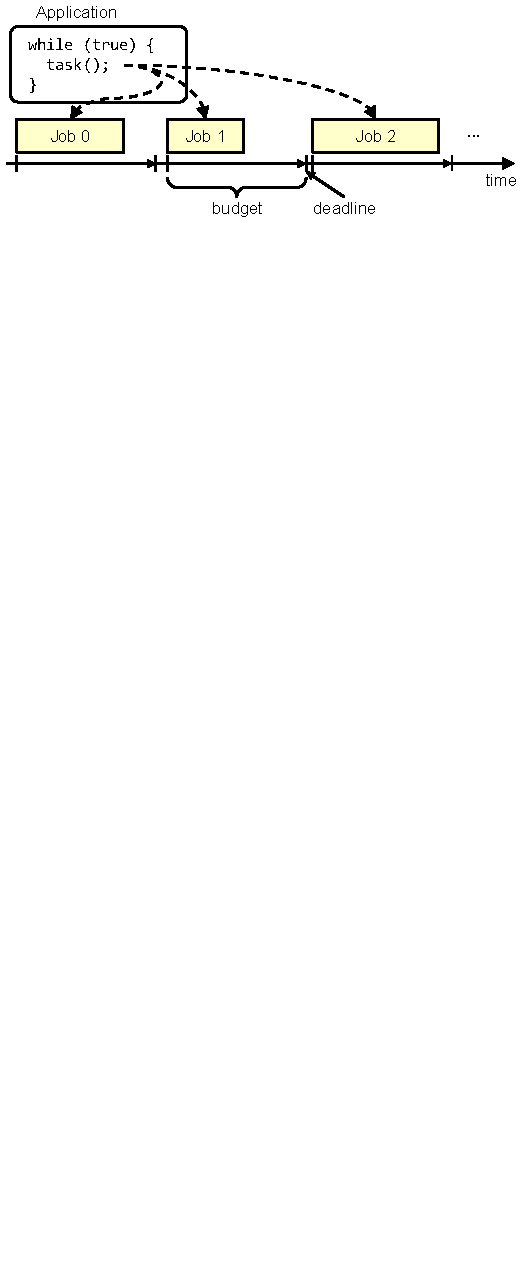
\includegraphics{exec_time_prediction/figs/jobs.pdf}
    \caption{Example of tasks, jobs, and deadlines.}
    \label{fig:applications.jobs}
  \end{center}
\end{figure}

We define a \emph{task} as a portion of an application that has an associated
response-time requirement. We refer to the time period in which it must
complete as its \emph{time budget}. For example, games are typically written with a
main task that
handles reading user input, updating game state, and displaying the output. In
order to maintain a certain frame rate (e.g., 30 frames per second), this task
must finish within the frame period budget (e.g., 33 milliseconds for 30
frames per second operation).

We define a \emph{job} as a dynamic instance of a task.
Figure~\ref{fig:applications.jobs} shows how a task maps to multiple jobs. Each
job has a deadline which is the time by which it must finish execution. For
example, for a game running at 30 frames-per-second, 30 jobs for the game loop
task are run each second. Each of these jobs has a deadline which is 33
milliseconds after the job's start time. These jobs all correspond to the same
set of static
task code, but their dynamic behavior differs due to different inputs and
program state. For example, one job may see that the user has pressed a button
and thus execute code to process this button press. Other jobs may see no new
user input and skip the need to process user input.  As a result, job execution
times can vary depending on input and program state.

\subsection{Variations in Execution Time}

% Execution time variation
\begin{figure}
  \begin{center}
    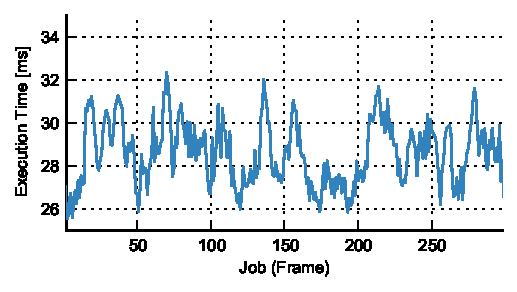
\includegraphics{exec_time_prediction/figs/ldecode_time.pdf}
    \caption{Execution time of jobs (frames) for ldecode (video decoder).}
    \label{fig:applications.ldecode_time}
  \end{center}
\end{figure}

These variations in execution times between jobs can be significant. 
Figure~\ref{fig:applications.ldecode_time} shows the execution time per job (frame) for
a video decoder application (ldecode) running on an ODROID-XU3 development board (see
Section~\ref{sec:evaluation} for full experimental setup). We can see that
there
are large variations in execution time from job to job due to differences in
input and program state when each job executes. Because of this large
variation, setting the appropriate DVFS level is a difficult problem. 

Using a
single DVFS level based on the average execution time (28.6 milliseconds) will
lead to a number of jobs missing their deadline. On the other hand, looking at the
worst-case execution time (32.3 milliseconds) implies that the application must
be run at its maximum frequency, which means that minimal energy saving from DVFS is
possible. Instead, the large variations from job to job imply that we need a
fine-grained, per-job decision of the DVFS level to use in order to minimize
energy usage while avoiding deadline misses.

\subsection{Existing DVFS Controllers}
\label{sec:apps.existing}

% Utilization
There are a large number of existing and proposed DVFS controllers. Most
controllers, such as the built-in Linux governors \cite{linux_governors}, adjust DVFS based on 
CPU utilization. When utilization is high, voltage and frequency are
increased, while when utilization is low, voltage and frequency are decreased.
This does not explicitly take into account deadlines and can result in high
energy usage or deadline misses. For example, high CPU utilization can cause a
high voltage and frequency level to be used. However, the time budget for the task
may actually be very long and a lower voltage and frequency would be
sufficient, resulting in lower energy usage. Similarly, CPU utilization for a
job could be low due to memory stalls, causing the controller to lower voltage
and frequency levels. However, if the task has a tight time budget, then this can
result in a deadline miss, whereas running at higher frequencies may have been
able to meet the deadline.
% This does not explicitly take into account deadlines and can result in high
% energy usage (e.g., running fast with a long deadline) or deadline
% misses (e.g., running slow with a tight deadline).

% RT
DVFS has been explored in hard real-time systems in order to save energy while
guaranteeing that deadlines are met \cite{rtdvfs-systor12}. In order to ensure
that deadlines are never missed, the analysis must be strictly conservative
which limits the amount of energy that can be saved. That is, a task will
always be run at a frequency such that even the slowest jobs will meet the
deadline. 
%For {\tt 2048} in Figure~\ref{fig:applications.2048},  this implies
%that all jobs must be run at maximum frequency.

% PID example
\begin{figure}
  \begin{center}
    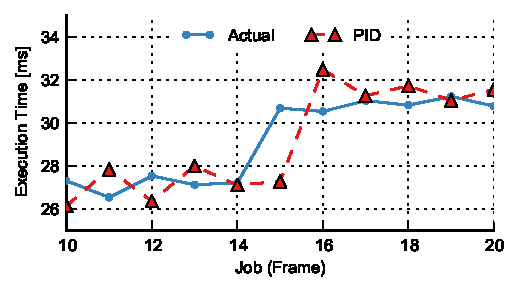
\includegraphics{exec_time_prediction/figs/ldecode_pid.pdf}
    \caption{Execution time of jobs (blue, solid) and execution time
    expected by a PID controller (red, dashed) for ldecode (video decoder).}
    \label{fig:applications.ldecode_pid}
  \end{center}
\end{figure}

% Workload
% Other work has explored characterizing workloads or phases in order to
% determine an appropriate DVFS level \cite{pacora-hotpar11, paragon-asplos13,
% quasar-asplos14}. These coarse-grained approaches use global or local
% average-case behavior in order to decide which DVFS level to use. This is not
% able to capture fine-grained job-to-job variations in execution times.
% Reactive
%Similarly, reactive controllers, such as PID-based control, are not able to
%respond in time to large fine-grained variations \cite{gu-dac08,
%pegasus-isca14, octopusman-hpca15, nachiappan-hpca15}.
%Figure~\ref{fig:applications.ldecode_pid} shows the expected execution times that a
%PID-based controller uses for setting the DVFS level and the real execution times of
%the jobs. As we can see, the PID controller's decision lags the actual
%execution times of the jobs.
Other work has explored using run-time information to inform DVFS control in
the presence of deadlines. These approaches are largely reactive and use
information about past job execution times to predict future job times
\cite{gu-dac08, choi-iccad02, pegasus-isca14, nachiappan-hpca15}. This can capture
coarse-grained phase changes in execution time, but cannot capture the
fine-grained job-to-job variations in execution times as the adjustment in DVFS
level happens too late.
For example, Figure~\ref{fig:applications.ldecode_pid} shows the expected
execution times that a PID-based controller uses for setting the DVFS level and
the real execution times of the jobs. As we can see, the PID controller's
decision lags the actual execution times of the jobs.

% Specific
More recently, people have investigated predicting job execution time and
setting DVFS in order to meet deadlines for specific applications (e.g., game rendering \cite{gu-rtas08}, web
browsing \cite{zhu-hpca13, eqos-hpca15}, web server/Memcached
\cite{adrenaline-hpca15}). These approaches involved careful analysis of the
application of interest, requiring extensive programmer effort, in order to
design the controller. As a result, the resulting controllers cannot be applied
to other applications.

\subsection{Prediction-Based Control}

% Prediction-based control overview
\begin{figure}
  \begin{center}
    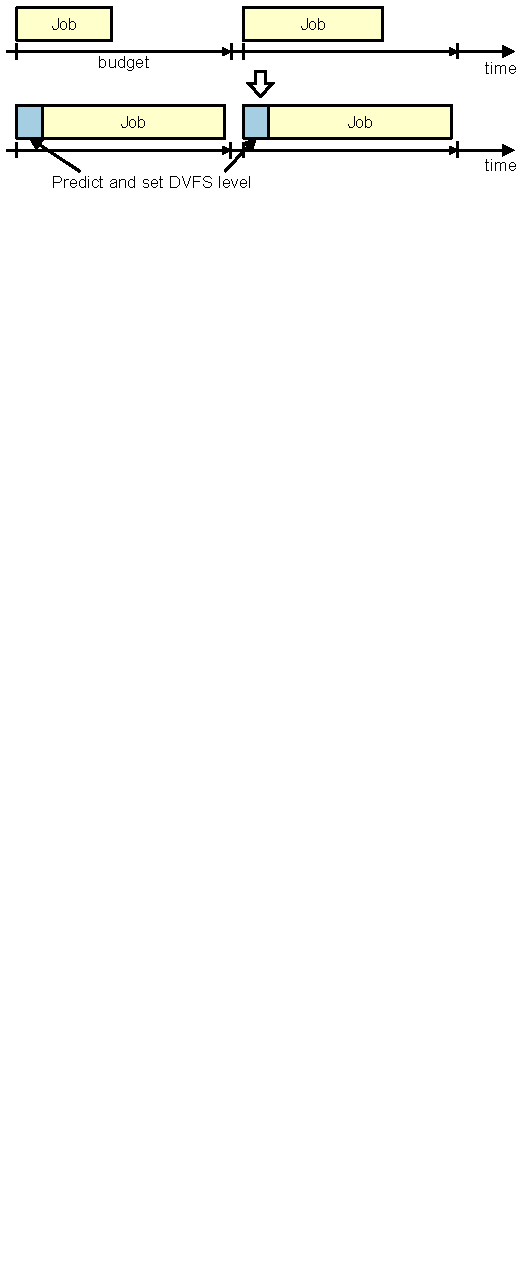
\includegraphics{exec_time_prediction/figs/prediction_overview.pdf}
    \caption{Overview of prediction-based control.}
    \label{fig:applications.prediction_overview}
  \end{center}
\end{figure}

Our goal in this work is to develop a general and automated framework in order to
create prediction-based DVFS controllers that can minimize energy usage without
missing deadlines.
Figure~\ref{fig:applications.prediction_overview} shows an overview of the operation of our
proposed prediction-based controller. The basic idea is to pre-pend tasks 
with a small segment of code. This segment of code will predict
the appropriate DVFS level to use for each of the task's jobs depending on the job's input and
current program state.

The main source of execution time variation between jobs is due to different
inputs and program state. Thus, the main challenge in developing a
prediction-based DVFS controller is determining how to map job input and
program state values to the appropriate DVFS frequency level. In general,
finding a direct mapping from input values to frequency levels is challenging
because the mapping can be irregular and complicated. In addition, this mapping
varies from application to application. For example, for one application,
pressing the ``down'' key may correspond to a large increase in execution time
while for other applications it may have no effect on execution time. Our
solution is to take advantage of the program source to give us hints about how
input values and program state will affect execution time. We use the program
source to automatically generate a prediction-based DVFS controller.

% Our goal in this work is to create a DVFS controller that sets the DVFS level
% for each job in such a way as to minimize energy usage without missing
% deadlines. In order to capture fine-grained variations in execution time, our
% controller needs to be proactive instead of reactive. That is, frequency needs
% to be increased before a long-running job begins in order to avoid deadline
% misses. In addition, the controller needs to be designed to be general across a
% wide-range of applications and largely automated with little need
% for programmer knowledge.

%Based on these previous controllers and our observations of large fine-grained
%variations in job execution time, our goal in this work is to create a
%controller with the following properties.
%\begin{enumerate}
%  \item \textbf{Proactive:} Control needs to be proactive instead of
%  reactive. That is, frequency needs to be increased/decreased before the
%  execution of a slow/fast job rather than after seeing such a job.
%  \item \textbf{Conservative:} The controller should aim to be conservative in
%  order to minimize deadline misses.
%  \item \textbf{General:} We aim to design a general methodology that is
%  applicable to a wide-range of applications without the need of detailed
%  programmer knowledge.
%  \item \textbf{Automated:} The methodology should be largely automated, with
%  limited need for programmer intervention.
%\end{enumerate}


\section{Execution Time Prediction for Energy-Efficiency}
\label{sec:prediction}

\subsection{Overview}
\label{sec:prediction.overview}

%The main challenge in developing our prediction-based controller is determining how to predict the
%appropriate frequency to use for each job. The main source of execution time
%variation between jobs is due to different inputs and program state. Thus, we
%need a model to map job input and program state values to frequency
%levels. In general, finding a direct mapping from input values to frequency levels
%is challenging because the mapping can be irregular and complicated. In
%addition, this mapping varies from application to application. For example, for
%one application, pressing the ``down'' key may correspond to a large increase
%in execution time while for other applications it may have no effect on execution
%time. 
%As a result,
%we break the prediction down into multiple steps and take advantage of the
%program source to give us hints about how input values and program state will
%affect execution time.

% Control flow graph
\begin{figure}
  \begin{center}
    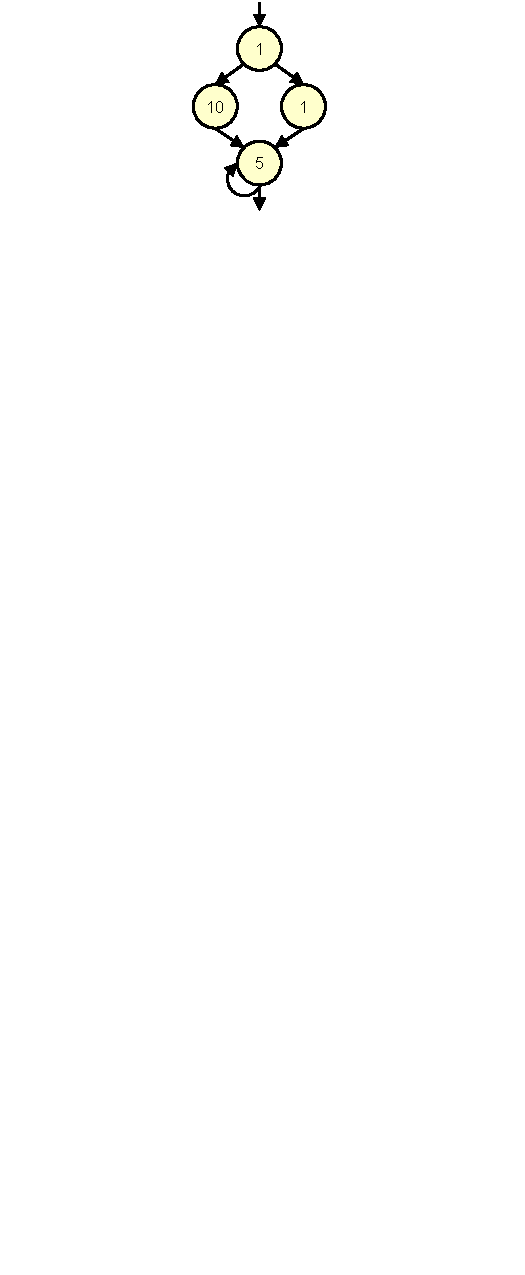
\includegraphics{exec_time_prediction/figs/cfg.pdf}
    \caption{Example control flow graph. Each node is annotated with its number of instructions.}
    \label{fig:prediction.cfg}
  \end{center}
\end{figure}

The basic intuition behind our prediction methodology is that, to first-order,
execution time correlates with the number of instructions run. Variations in
the number of instructions run are described by the control flow taken by a
specific job. For example, consider the control flow graph for a task shown in
Figure~\ref{fig:prediction.cfg}. Each node is marked with its number of instructions.
Taking the left branch instead of the right
branch corresponds to nine more instructions being executed. Similarly, each
additional loop iteration of the last basic block adds five instructions to the
number of instructions executed. By knowing which branch is taken and the
number of loop iterations, we can know the number of instructions
executed and estimate the execution time. 
With an estimate of the execution time, we can then estimate the performance-scaling impact of DVFS and choose
an appropriate frequency and voltage level to run at in order to just
meet the deadline.

% Prediction flow
\begin{figure}
  \begin{center}
    \includegraphics{exec_time_prediction/figs/prediction_flow.pdf}
    \caption{Steps to predict execution time from job input and program state.}
    \label{fig:prediction.prediction_flow}
  \end{center}
\end{figure}

Figure~\ref{fig:prediction.prediction_flow} shows the main steps in our
prediction method. We first instrument the task source code and use program
slicing to create a code fragment that will
calculate control flow features for a job. The code fragment is run before a
job executes in order to generate the control flow features
(Section~\ref{sec:prediction.features}). Next, we use a linear model, which we train off-line, to map
control flow features to an execution time estimate for the job 
(Section~\ref{sec:prediction.model}). Finally, we use classical linear models \cite{xie-pldi03, wu-micro05}
that describe the frequency-performance trade-off of DVFS to select an
appropriate frequency (Section~\ref{sec:prediction.dvfs}).

\subsection{Program Features}
\label{sec:prediction.features}

% Example insertion of feature counters
\begin{figure}
  \begin{center}
    \includegraphics{exec_time_prediction/figs/features.pdf}
    \caption{Example of feature counters inserted for conditionals, loops, and function calls.}
    \label{fig:prediction.features}
  \end{center}
\end{figure}

The first step needed for our prediction is to generate control flow features.
That is, we want to know the control flow of a task when executing with a
specific input and program state.
For this purpose, we instrument the task source to count these control flow features.
Specifically, we instrument the task to count the following features:
\begin{itemize}
  \item Number of iterations for each loop
  \item Number of times each conditional branch is taken
  \item Address of each function pointer call
\end{itemize}
Figure~\ref{fig:prediction.features} shows examples of how these features are
instrumented. 
We focus on control flow features because these explain 
most of the execution time variation. However, other features, such as variable
values or memory accesses, could be included to improve the prediction
accuracy.

% Add loop counters, slice
\begin{figure*}
  \begin{center}
    \includegraphics{exec_time_prediction/figs/code_transformations.pdf}
    \caption{Example of program slicing for control flow features.}
    \label{fig:prediction.code_transformations}
  \end{center}
\end{figure*}

Generating these features using an instrumented version of the task code is not
suitable for prediction because the instrumented task will take at least as long
as the original task to run. Instead, we need to quickly generate these features before
the task execution. In order to minimize the prediction execution time, we use
program slicing to produce the minimal code needed to calculate these features.
Figure~\ref{fig:prediction.code_transformations} shows a simple example of this
flow. By removing the actual computation and only running through the control
flow, the execution time can be greatly reduced. We refer to the resulting
program slice that computes the control flow
features as the \emph{prediction slice} or simply as the \emph{slice}.

One problem that arises with running this prediction slice before a task is the
issue of side-effects. That is, the slice could write to global variables and
break the correctness of the program. In order to prevent this, the slice
creates local copies of any global variables that are used. Values for these
local copies are updated at the start of the slice and writes are only applied
to the local copy. A similar process is applied to any arguments that are
passed by reference.

\subsection{Execution Time Prediction Model}
\label{sec:prediction.model}

% Runtime power of monitoring core
\begin{table}[tb]
  \begin{center}
    \begin{small}
    \begin{tabular}{|c|l|l|}

\hline
Variable & Type & Description \\ \hline\hline
$\bar{y}$ & Scalar & Predicted execution time \\ \hline
$\textbf{x}$ & Vector & Feature values \\ \hline
$\boldsymbol{\beta}$ & Vector & Model coefficients \\ \hline\hline
$\textbf{y}$ & Vector & Profiled execution times \\ \hline
$\textbf{X}$ & Matrix & Profiled feature values \\ \hline
$\textbf{X}\boldsymbol{\beta} - \textbf{y}$ & Vector & Prediction errors \\ \hline\hline
$\alpha$ & Scalar & Under-predict penalty weight \\ \hline
$\gamma$ & Scalar & Number of terms penalty weight \\ \hline
$\|\cdot\|$ & Scalar & L2-norm (sum of squares) \\ \hline
$\|\cdot\|_1$ & Scalar & L1-norm (sum of absolute values) \\ \hline

\end{tabular}


    \end{small}
    \caption{Variable and notation descriptions.}
    \label{tab:prediction.variables}
  \end{center}
\end{table}

Next, we need to predict the execution time from the control flow features.  This section
describes our model that maps features to execution time.
Table~\ref{tab:prediction.variables} summarizes the variables and
notation that are used in this section. 
We use a linear model to map features to execution time as this captures the
basic correlation. 
Higher-order or non-polynomial models may provide better accuracy.
However, a linear model has the advantage of being both simple to
train and fast to evaluate at run-time. In addition, it is always convex which
allows us to use convex optimization-based methods to fit the model.
Our linear model can be expressed as
\begin{align*}
  \bar{y} = \mathbf{x} \boldsymbol{\beta}
\end{align*}
where $\bar{y}$ is the predicted execution time, $\mathbf{x}$ is a vector of
feature values, and $\boldsymbol{\beta}$ are the coefficients that map feature
values to execution time. These $\boldsymbol{\beta}$ coefficients are
fit using profiling data. Specifically, we profile the program to
produce a set of training data consisting of execution times $\mathbf{y}$ and
feature vectors $\mathbf{X}$ (i.e., each row of $\mathbf{X}$ is a vector of
features, $\mathbf{x}_i$, for one job). Note that in order to achieve the expected linear
correlation between features and execution time, addresses recorded for
function calls are converted to a one-hot encoding indicating whether particular
function addresses were called or not.

The most common way to fit a linear model is to use linear least squares regression.
Linear least squares regression finds the coefficients $\boldsymbol{\beta}$ that minimize the mean
square error:
\begin{align*}
\begin{aligned}
  \underset{\boldsymbol{\beta}}{\text{argmin}} & & \|\mathbf{X}\boldsymbol{\beta} - \textbf{y}\|^2
\end{aligned}
\end{align*}
Essentially, this aims to minimize the sum of the absolute errors in the
prediction. That is, it weights negative and positive errors equally. However,
these two errors lead to different behaviors on our system.
Negative errors (under-prediction) lead to deadline misses since we predict the
job to run faster than its actual execution time. On the other hand, positive errors
(over-prediction) result in an overly conservative frequency setting which does
not save as much energy as possible. In order to maintain a good user
experience, we would prefer to avoid deadline misses, possibly at the cost of
energy usage. In other words, we should place greater weight on avoiding
under-prediction as opposed to over-prediction.

We can place greater weight on under-prediction by modifying our optimization objective:
\begin{align*}
\begin{aligned}
  \underset{\boldsymbol{\beta}}{\text{argmin}} & & \|pos(\textbf{X}\boldsymbol{\beta} - \textbf{y})\|^2 + \alpha \|neg(\textbf{X}\boldsymbol{\beta} - \textbf{y})\|^2
\end{aligned}
\end{align*}
where $pos(x) = max\{x, 0\}$ and $neg(x) = max\{-x, 0\}$ and these functions are applied
element-wise to vectors. Thus, $\|pos(\textbf{X}\boldsymbol{\beta} -
\textbf{y})\|^2$ represents the over-prediction error and
$\|neg(\textbf{X}\boldsymbol{\beta} - \textbf{y})\|^2$ represents the
under-prediction error. $\alpha$ is a weighting factor that allows us to place a
greater penalty on under-predictions by setting $\alpha > 1$.
Since this objective is convex, we can use existing convex optimization solvers
to solve for $\boldsymbol{\beta}$.

Coefficients which are zero imply that the corresponding control flow features
do not need to be calculated by the prediction slice. We can use this
information to further reduce the size and execution time of the prediction
slice. We can extend our optimization objective to favor using less features
by using the Lasso method \cite{lasso-jrss96}:
\begin{align*}
\begin{aligned}
  \underset{\boldsymbol{\beta}}{\text{argmin}} & & \|pos(\textbf{X}\boldsymbol{\beta} - \textbf{y})\|^2 + \alpha \|neg(\textbf{X}\boldsymbol{\beta} - \textbf{y})\|^2 + \gamma \|\boldsymbol{\beta}\|_1
\end{aligned}
\end{align*}
where $\|\cdot\|_1$ is the L1-norm and $\gamma$ is a weighting factor that
allows us to trade-off prediction accuracy with the number of features needed.

\subsection{DVFS Model}
\label{sec:prediction.dvfs}

% DVFS linearity
\begin{figure}
  \begin{center}
    \includegraphics{exec_time_prediction/figs/dvfs_linearity.pdf}
    \caption{Average execution time of jobs (frames) for ldecode (video
    decoding) as frequency level varies.}
    \label{fig:prediction.dvfs_linearity}
  \end{center}
\end{figure}

Given a predicted execution time, we need to
estimate how the execution time will change with varying frequency. For this,
we use the classical linear model found in literature \cite{xie-pldi03, wu-micro05}:
\begin{align*}
  t = T_{mem} + N_{dependent}/f
\end{align*}
where $t$ is the execution time, $T_{mem}$ is the memory-dependent execution time
that does not scale with frequency, $N_{dependent}$ is the number of CPU cycles
that do not overlap with memory and scale with frequency, and $f$ is
the frequency.
In order to verify this linearity assumption, we measured average job execution
times as frequency was varied. Figure~\ref{fig:prediction.dvfs_linearity} shows
the average job execution time versus $1/f$ for ldecode (video decoder
application). We can see that $t$ and $1/f$ do show a linear relationship. We
saw similar results for the other applications we tested.

For this linear model, by predicting the execution time at two points, we can
determine $T_{mem}$ and $N_{dependent}$ 
for a job and calculate the minimum frequency $f$ to satisfy a
given time budget $t_{budget}$. More specifically, we predict the execution time
$\bar{t}_{fmin}$ at minimum frequency $f_{min}$ and the execution time
$\bar{t}_{fmax}$ at maximum frequency $f_{max}$. Using these two points, we can calculate $T_{mem}$ and $N_{dependent}$ as
\begin{align*}
  N_{dependent} &= \frac{f_{min}f_{max}(\bar{t}_{fmin} - \bar{t}_{fmax})}{f_{max} - f_{min}} \\
  T_{mem} &= \frac{f_{max}\bar{t}_{fmax} - f_{min}\bar{t}_{fmin}}{f_{max} - f_{min}}
\end{align*}

For a given budget $t_{budget}$, we want the minimum frequency $f_{budget}$ that will meet this time. This can be calculated as
\begin{align*}
  f_{budget} = \frac{N_{dependent}}{t_{budget} - T_{mem}}
\end{align*}

Since execution time can vary even with the same job inputs and program state, 
we add a margin to the predicted execution times used
($t_{fmin}$ and $t_{fmax}$). In our experiments we used a margin of 10\%. A
higher margin can decrease deadline misses while a lower margin can improve the
energy savings. 
The resulting predicted frequency is the exact frequency that we expect will just satisfy the
time budget. However, DVFS is only supported for a set of
discrete frequency levels. Thus, the actual frequency we select is the smallest
frequency allowed that is greater than $f_{budget}$. 

% Effective budget
\begin{figure}
  \begin{center}
    \includegraphics{exec_time_prediction/figs/effective_budget.pdf}
    \caption{The effective budget decreases due to slice and DVFS execution time.}
    \label{fig:prediction.effective_budget}
  \end{center}
\end{figure}

% DVFS switching time
\begin{figure}
  \begin{center}
    \includegraphics{exec_time_prediction/data/dvfs_heatmap.pdf}
    \caption{95th-percentile switching times for DVFS.}
    \label{fig:prediction.dvfs_heatmap}
  \end{center}
\end{figure}

The execution of the prediction slice and DVFS switch
reduces the amount of time available for a job to execute and still satisfy its
budget. Thus, the effective budget when choosing a frequency to run at
needs to consider these overheads (see
Figure~\ref{fig:prediction.effective_budget}). Although the execution time of
the prediction slice can be measured, the DVFS switching time must be
estimated, as the switch has not been performed yet.  This is done by
microbenchmarking the DVFS switching time.
Figure~\ref{fig:prediction.dvfs_heatmap} shows the 95th-percentile DVFS
switching times for our test platform for each possible start and ending
frequency. We use the 95th-percentile switching times in order to be
conservative in our estimate of DVFS switching time while omitting rare
outliers. 
%As the switching time depends on the start and end frequencies, we
%search through the target frequencies to find the minimal frequency that will
%satisfy the time budget, taking into account the slice and DVFS times.

% If the portion of the job that does not scale with frequency is negligible
% (i.e., $T_{mem} \approx 0$), then we only need to profile at one point and
% $N_{dependent}$ simplifies to
% \begin{align*}
%   N_{dependent} &= t_{fmax}f_{max}
% \end{align*}
% and the frequency calculation simplifies to
% \begin{align*}
%   f_{deadline} = \frac{N_{dependent}}{t_{deadline}} = \frac{t_{fmax}f_{max}}{t_{deadline}}
% \end{align*}
% For the applications we tested, we found $T_{mem}$ to be negligible. Thus, we
% were able to select an appropriate DVFS level with only one predicted execution
% time (at $f_{max}$).

\subsection{Alternate Prediction Models}

In this section, we have described our specific prediction strategy for each
step in our overall prediction flow shown in
Figure~\ref{fig:prediction.prediction_flow}. However, we note that each step in
this prediction flow can be substituted with alternate models as long as it
produces the needed prediction for the next step.
The most obvious change would be to use more complex prediction models for each
step (e.g., more features generated and higher-order, non-linear models).
For the benchmarks we evaluated, we saw relatively little gain to be had from
improved prediction (see Section~\ref{sec:evaluation.overheads}) and thus the
increased overheads of more complex models were not justified.
Instead, we discuss here some alternative extensions.

For feature generation, we have focused on automated generation in order for
the approach to be general and limit the need for domain-specific expertise.
However, this does not preclude the programmer from manually adding ``hints''
that they expect would correlate well with a job's execution time. For example,
the programmer may be able to extract meta-data from input files and manually
encode these to features.

%For our prediction-based DVFS controller, we focused on control flow features
%as these describe most of the execution time variation. Additional features may
%improve prediction accuracy for certain applications. For example,
%cache-sensitive applications may want to include features related to memory
%accesses. For multi-threaded applications, number of threads and features
%related to possible parallelism could be useful. In addition, the programmer
%could add ``hint'' features that they expect would correlate well with a
%job's execution time. For example, if they know that certain user inputs will
%correlate to high execution time, they could explicitly code these as features
%in the prediction slice.

One interesting extension to execution time prediction involves its use in
feature selection. Additional constraints could be added to the execution
time prediction in order to limit the use of features which require high
overhead to generate. Features over some overhead threshold could
be explicitly disallowed or the overhead for each feature could be
introduced as penalties in the optimization objective.
%For execution time prediction, many options exist including higher-order, non-linear
%models or machine-learning based approaches such as artificial neural networks.
% However, these approaches introduce both increased training time and on-line
% execution times. As this time reduces the effective deadline, the improvement
% in prediction accuracy needs to be large enough to justify the overhead.

The last step in our flow focuses on selecting an appropriate
frequency level for DVFS control. However, this last step could be substituted to
support other performance-energy trade-off mechanisms, such as heterogeneous
cores. By using alternate models for how the execution time scales with the
performance-energy trade-off mechanism, an appropriate operating point can be
selected for the mechanism of interest.

\section{System-Level Framework}
\label{sec:exec_time_prediction.system}

This section describes the overall framework and operation of our
prediction-based controller.

\subsection{Programmer Annotation}

% Programmer annotation
\begin{figure}
  \begin{center}
    \includegraphics{exec_time_prediction/figs/programmer_annotation.pdf}
    \caption{Example of programmer annotation to mark task boundaries and time
    budgets.}
    \label{fig:exec_time_prediction.system.programmer_annotation}
  \end{center}
\end{figure}

In order to identify tasks and their time budgets, programmer annotation is
required. The programmer must annotate the start and the end of a task and the
desired response-time requirement.
Figure~\ref{fig:exec_time_prediction.system.programmer_annotation} shows an
example of this annotation.  For ease of analysis and to ensure that tasks that
start always end, we require the start and end of a task to be within one
function.  Arbitrary code paths can be modified to fit this model by using a
wrapper function or re-writing the code. Multiple non-overlapping tasks can be
supported, though we only considered one task in the applications we tested.

\subsection{Off-line Analysis}

% High-level flow of framework
\begin{figure*}
  \begin{center}
    \includegraphics{exec_time_prediction/figs/high_level_flow.pdf}
    \caption{Overall flow for prediction-based DVFS control.}
    \label{fig:exec_time_prediction.system.high_level_flow}
  \end{center}
\end{figure*}

Figure~\ref{fig:exec_time_prediction.system.high_level_flow} shows the overall
flow of our framework for creating prediction-based DVFS controllers. Given
programmer annotation to identify tasks, we can automatically instrument these
tasks to record control flow features. Off-line, we profile these tasks in
order to collect traces of feature values and job execution times.  This is
used to train our execution time prediction model, as described in
Section~\ref{sec:exec_time_prediction.prediction.model}. Since execution time
depends on the specific hardware and platform that an application is run on,
profiling and model training needs to be done for the platform that the
application will be run on. For common platforms, the program developer can
perform this profiling and distribute the trained model coefficients with the
program. Alternatively, profiling can be done by the user during the
application's installation.

% Differences in slice features
\begin{table*}
  \begin{center}
    \begin{footnotesize}
    \begin{tabular}{|l|l|r|r|r|}

\hline
\multirow{2}{*}{\bf Platform} & \multirow{2}{*}{\bf Benchmark} & \multirow{2}{*}{\bf Feature Diff} & \multicolumn{2}{r|}{\bf Prediction Diff} \\ \cline{4-5}
& & & {\bf Average} & {\bf Max} \\ \hline\hline

\multirow{8}{*}{ARM-big}
& 2048         & --     & 0\%   & 0\%   \\ \cline{2-5}
& curseofwar   & --     & 0\%   & 0\%   \\ \cline{2-5}
& ldecode      & --     & 0\%   & 0\%   \\ \cline{2-5}
& pocketsphinx & --     & 0\%   & 0\%   \\ \cline{2-5}
& rijndael     & --     & 0\%   & 0\%   \\ \cline{2-5}
& sha          & --     & 0\%   & 0\%   \\ \cline{2-5}
& uzbl         & --     & 0\%   & 0\%   \\ \cline{2-5}
& xpilot       & -2, +1 & 0.1\% & 8.7\% \\ \hline\hline

\multirow{8}{*}{x86}
& 2048         & +67    & 0.4\% & 2.9\% \\ \cline{2-5}
& curseofwar   & --     & 0\%   & 0\%   \\ \cline{2-5}
& ldecode      & --     & 0\%   & 0\%   \\ \cline{2-5}
& pocketsphinx & +2     & 0\%   & 0\%   \\ \cline{2-5}
& rijndael     & --     & 0\%   & 0\%   \\ \cline{2-5}
& sha          & --     & 0\%   & 0\%   \\ \cline{2-5}
& uzbl         & -1     & 0\%   & 0\%   \\ \cline{2-5}
& xpilot       & +6, -8 & 0.7\% & 2.9\% \\ \hline 

\end{tabular}

    \end{footnotesize}
    \caption{Differences in features selected and predicted execution times for
    different platforms compared to an ARM-LITTLE platform.}
    \label{tab:exec_time_prediction.system.slice_differences}
  \end{center}
\end{table*}

The trained execution time model only requires a subset of all the features to
perform prediction. Thus, this information is used to eliminate code for
calculating unneeded features.  Program slicing is then used to create a
minimal code fragment to calculate the needed control flow features.  Note that
since the features needed depends on the training of the execution time
prediction model, which is platform-dependent, the features needed could vary
across platforms. However, we expect the features that are needed are
primarily a function of the task semantics (i.e., execution time variations
across control paths) rather than the platform it is run on. In fact, we
compared the predictions made for an x86-based (Intel Core i7) platform when
using the features selected for an ARM LITTLE-based ODROID-XU3 platform and for the
features selected for the x86 platform itself. We also compared using the ARM
big core compared to the LITTLE core on the ODROID-XU3 platform. 
Table~\ref{tab:exec_time_prediction.system.slice_differences} shows the
features that are added or removed in the prediction slices for these platforms
compared to the prediction slice generated for the ARM LITTLE core. In
addition, the differences in predicted execution times using the prediction
slice generated for the platform and using the prediction slice from the ARM
LITTLE core are shown. 
For the ARM big core, only one benchmark shows differences in features selected
with the resulting difference in prediction times being only 0.1\% on average.
For the x86-based platform, four benchmarks show differences in features
selected. In two of these cases, the predicted execution times are not
affected. In the remaining two cases, average differences in predicted
execution times are less than 1\%.
%For all but three of the
%benchmarks we tested, the features selected were exactly the same.  For one of
%these, the features selected by the x86 platform were a subset of those
%selected by the ARM platform and so the predicted times were exactly the same.
%For the remaining two benchmarks, the predicted times differed by less than
%3\%. 
Although we had to re-train the execution time model coefficients for these new
platforms, the same prediction slice was applicable across both platforms.

\subsection{Run-time Prediction}

% Slice operation choices
\begin{figure}
  \begin{center}
    \includegraphics{exec_time_prediction/figs/predictor_operation.pdf}
    \caption{Options for how to run predictor.}
    \label{fig:exec_time_prediction.system.predictor_operation}
  \end{center}
\end{figure}

The prediction slice, execution time predictor, and frequency predictor are
combined to form the \emph{DVFS predictor} or simply \emph{predictor} There are
several options for how to run the predictor in relation to jobs.
Figure~\ref{fig:exec_time_prediction.system.predictor_operation} shows some of
these options.  The simplest approach is to run the slice just before the
execution of a job. This uses up part of the time budget to execute the predictor, as
mentioned in Section~\ref{sec:exec_time_prediction.prediction.dvfs}. However,
if this time is low, then the impact is minimal.

An alternative option would be to run the predictors and jobs in a parallel,
pipelined manner such that during job $i$, the predictor for job $i+1$ is run.
This ensures that the DVFS decision is ready at the start of a job with no
impact on time budget from the predictor. Due to the longer time budget,
running in a pipelined manner can save more energy than running in a sequential
manner. However, this assumes that
information needed by the prediction slice, specifically the job inputs and
program state, is ready one job in advance. This is not possible for
interactive tasks which depend on real-time user inputs or tasks which are not
periodic.

The predictor could also be run in parallel with the task. This avoids the
issue of needing input values early. In terms of time budget, this mode of
operation still reduces the effective budget by the predictor execution time.
However, part of the task also executes during the prediction time, so the
remaining work to be done is also reduced. Thus, this could still lead to
higher energy savings than running in a sequential manner.
Running in parallel also avoids the issue of side-effects
caused by the prediction slice that was discussed in
Section~\ref{sec:exec_time_prediction.prediction.features}. However, running in
parallel either requires forking off the predictor for each job or sharing data
with a dedicated predictor thread, both of which can introduce overhead.

For our target applications, we found that the execution time of the predictor
was low. Thus, we decided to run the predictor and task in a sequential manner
(i.e., ``Sequential'' in
Figure~\ref{fig:exec_time_prediction.system.predictor_operation})
For applications which require more complicated predictors, these alternative
operation modes may be beneficial.

\section{Evaluation}
\label{sec:exec_time_prediction.evaluation}

\subsection{Experimental Setup}
\label{sec:exec_time_prediction.evaluation.setup}

% Benchmark descriptions
\begin{table*}
  \begin{center}
    \begin{footnotesize}
    \begin{tabular}{|l||l|l||r|r|r|}

\hline
\multirow{2}{*}{\bf Benchmark} & \multirow{2}{*}{\bf Description} & \multirow{2}{*}{\bf Task} & \multicolumn{3}{c|}{\bf{Job Times [ms]}} \\ \cline{4-6}
& & & {\bf Min} & {\bf Avg} & {\bf Max} \\ \hline\hline


2048 \cite{2048} & Puzzle game & Update and render one turn &
  0.52 & 1.2 & 2.1 \\ \hline
curseofwar \cite{curseofwar} & Real-time strategy game & Update and render one game loop iteration &
  0.02 & 6.2 & 37.2 \\ \hline
ldecode \cite{ldecode} & H.264 decoder & Decode one frame & 
  6.2 & 20.4 & 32.5 \\ \hline
pocketsphinx \cite{pocketsphinx-icassp06} & Speech recognition & Process one speech sample & 
  718 & 1661 & 2951 \\ \hline
rijndael \cite{mibench} & Advanced Encryption Standard (AES) & Encrypt one piece of data & 
  14.2 & 28.5 & 43.6 \\ \hline
sha \cite{mibench} & Secure Hash Algorithm (SHA) & Hash one piece of data & 
  4.7 & 25.3 & 46.0 \\ \hline
%stringsearch \cite{mibench} & Search for words in phrases & Perform a set of searches \\ \hline
uzbl \cite{uzbl} & Web browser & Execute one command (e.g., refresh page) & 
  0.04 & 2.2 & 35.5 \\ \hline
xpilot \cite{xpilot} & 2D space game & Update and render one game loop iteration & 
  0.2 & 1.3 & 3.1 \\ \hline


\end{tabular}

    \end{footnotesize}
    \caption{Benchmark descriptions and task of interest.}
    \label{tab:exec_time_prediction.evaluation.benchmarks}
  \end{center}
\end{table*}

% Benchmark execution times
\begin{table*}
  \begin{center}
    \begin{footnotesize}
    \begin{tabular}{|l|r|r|r|}

\hline
{\bf Benchmark} & {\bf Min [ms]} & {\bf Avg. [ms]} & {\bf Max [ms]} \\ \hline\hline

2048         & 0.52 &  1.2 &  2.1 \\ \hline
curseofwar   & 0.02 &  6.2 & 37.2 \\ \hline
ldecode      & 6.2  & 20.4 & 32.5 \\ \hline
pocketsphinx & 718  & 1661 & 2951 \\ \hline
rijndael     & 14.2 & 28.5 & 43.6 \\ \hline
sha          & 4.7  & 25.3 & 46.0 \\ \hline
uzbl         & 0.04 & 2.2  & 35.5 \\ \hline
xpilot       & 0.2  & 1.3  & 3.1 \\ \hline

\end{tabular}

    \end{footnotesize}
    \caption{Execution time statistics when running
    at maximum frequency.}
    \label{tab:exec_time_prediction.evaluation.job_statistics}
  \end{center}
\end{table*}

We applied our framework for prediction-based DVFS control to a set of eight
benchmark applications including three games, a web browser, speech
recognition, a video decoder and two applications from the MiBench suite
\cite{mibench}.  Table~\ref{tab:exec_time_prediction.evaluation.benchmarks}
lists and describes these benchmarks and the task of interest for each.
Table~\ref{tab:exec_time_prediction.evaluation.job_statistics} shows the
minimum, average, and maximum job execution times for these benchmarks when run
at maximum frequency.

We ran our experiments on an ODROID-XU3 \cite{odroid} development board running
Ubuntu 14.04. The ODROID-XU3 includes a Samsung Exynos5422 SoC with ARM
Cortex-A15 and Cortex-A7 cores. We show results here for running on the more
power-efficient A7 core but we saw similar trends when running on the A15 core.
In order to isolate measurements for the application of interest, we pinned the
benchmark to run on the A7 core while using the A15 to run OS and background
jobs. We measured power using the on-board power sensors with a sampling rate
of 213 samples per second and integrated over time to calculate energy usage.

We compare our proposed prediction-based DVFS controller with existing
controllers and previously proposed control schemes. Specifically, we measure
results for the following DVFS schemes:
\begin{enumerate}
  \item \textbf{performance}: The Linux performance governor
  \cite{linux_governors} always runs at the maximum frequency. We normalize our
  energy results to this case.
  \item \textbf{interactive}: The Linux interactive governor
  \cite{linux_governors} was designed for interactive mobile applications. It
  samples CPU utilization every 80 milliseconds and changes to maximum
  frequency if CPU utilization is above 85\%.
  \item \textbf{pid}: The PID-based controller uses previous prediction errors
  with a PID control algorithm in order to predict the execution time of the
  next job \cite{gu-dac08}. The PID parameters are trained offline and are
  optimized to reduce deadline misses.
  \item \textbf{prediction}: This is our prediction-based controller as
  described in this paper.
\end{enumerate}

\subsection{Energy Savings and Deadline Misses}

% Energy, deadline misses
\begin{figure*}
  \begin{center}
    \includegraphics{exec_time_prediction/data/em_summary.pdf}
    \caption{Normalized energy usage and deadline misses.}
    \label{fig:exec_time_prediction.evaluation.em_summary}
  \end{center}
\end{figure*}

Figure~\ref{fig:exec_time_prediction.evaluation.em_summary} compares energy
consumption and deadline misses for the different DVFS controllers across our
benchmark set. These experiments are run with a time budget of 50 ms per job as
running faster than this is not noticeable to a user \cite{lindgaard-bit06,
eqos-hpca15}.  pocketsphinx takes at least 100s of milliseconds to run (see
Table~\ref{tab:exec_time_prediction.evaluation.benchmarks}) so we use a 4
second deadline. This corresponds to the time limit that a user is willing to
wait for a response \cite{miller-afips68}.  Energy numbers are normalized to
the energy usage of the performance governor.  Deadline misses are reported as
the percentage of jobs that miss their deadline. 

We see that, on average, our prediction-based controller saves 56\% energy
compared to running at max frequency. This is 27\% more savings than the
interactive governor and 1\% more savings than the PID-based controller.  For
ldecode, pocketsphinx, and rijndael, prediction-based control shows higher
energy consumption than PID-based control. However, if we look at deadline
misses, we see that PID-based control shows a large number of misses for these
benchmarks. On average, the interactive governor shows 2\% deadline misses and
the PID-based controller shows 13\% misses. In contrast, our prediction-based
controller shows 0.1\% deadline misses for curseofwar and no deadline misses
for the other benchmarks tested. Overall, we see that the interactive governor
has a low number of deadline misses, but achieves this with high energy
consumption. On the other hand, PID-based control shows lower energy usage than
the prediction-based controller in some cases, but this comes at the cost of a
large number of deadline misses. Instead, on average, our prediction-based
control is able to achieve both better energy consumption and less deadline
misses than the interactive governor and PID-based control.

% Deadline sweeps
\begin{figure*}
  \begin{center}
  \begin{subfigure}[2048]{
    \includegraphics{exec_time_prediction/data/2048.pdf}
  }
  \end{subfigure}
  \begin{subfigure}[curseofwar]{
    \includegraphics{exec_time_prediction/data/curseofwar.pdf}
  }
  \end{subfigure}

  \begin{subfigure}[ldecode]{
    \includegraphics{exec_time_prediction/data/ldecode.pdf}
  }
  \end{subfigure}
  \begin{subfigure}[pocketsphinx]{
    \includegraphics{exec_time_prediction/data/pocketsphinx.pdf}
  }
  \end{subfigure}

  \begin{subfigure}[rijndael]{
    \includegraphics{exec_time_prediction/data/rijndael.pdf}
  }
  \end{subfigure}
  \begin{subfigure}[sha]{
    \includegraphics{exec_time_prediction/data/sha.pdf}
  }
  \end{subfigure}

  \begin{subfigure}[uzbl]{
    \includegraphics{exec_time_prediction/data/uzbl.pdf}
  }
  \end{subfigure}
  \begin{subfigure}[xpilot]{
    \includegraphics{exec_time_prediction/data/xpilot.pdf}
  }
  \end{subfigure}

  \caption{Normalized energy usage and deadline misses as time budget is
  varied.}
  \label{fig:exec_time_prediction.evaluation.sweeps}
  \end{center}
\end{figure*}

Since our prediction-based controller takes the time budget into account, it is
able to save more energy with longer time budgets. Similarly, with shorter time
budgets, it will spend more energy to attempt to meet the tighter deadlines.
In order to study this trade-off, we swept the time budget around the point
where we expect to start seeing deadline misses. Specifically, we set a
normalized budget of 1 to correspond to the maximum execution time seen for the
task when running at maximum frequency (see
Table~\ref{tab:exec_time_prediction.evaluation.benchmarks}). This corresponds
to the tightest budget such that all jobs are able to meet their deadline.
Figure~\ref{fig:exec_time_prediction.evaluation.sweeps} shows the energy usage
and deadline misses for the various benchmarks as the normalized budget is
swept below and above 1.  We see that our prediction-based controller is able
to save more energy with longer time budgets and continues to outperform the
interactive governor and the PID-based controller for varying time budgets.
For normalized budgets less than 1, our prediction-based controller shows
deadline misses. However, the number of misses is typically close to the number
seen with the performance governor.  This implies that the only deadline misses
are the ones that are impossible to meet at the specified time budget, even
with running at the maximum frequency.

\subsection{Analysis of Overheads and Error}
\label{sec:exec_time_prediction.evaluation.overheads}

% Overhead time
\begin{figure}
  \begin{center}
    \includegraphics{exec_time_prediction/data/overhead_time.pdf}
    \caption{Average time to run prediction slice and switch DVFS levels.}
    \label{fig:exec_time_prediction.evaluation.overhead_time}
  \end{center}
\end{figure}

Figure~\ref{fig:exec_time_prediction.evaluation.overhead_time} shows the
average times for executing the predictor and for switching DVFS levels.  On
average, the predictor takes 3.2 ms to execute and DVFS switching takes 0.8 ms.
Excluding pocketsphinx, the average total overhead is less than 1 ms which is
2\% of a 50 ms time budget.  pocketsphinx shows a long execution time for the
predictor. However, this time is negligible compared to the execution time of
pocketsphinx jobs which are on the order of seconds.

% Results w/o overhead
\begin{figure}
  \begin{center}
    \includegraphics{exec_time_prediction/data/overhead_comparison.pdf}
    \caption{Normalized energy usage and deadline misses with overheads removed
    and oracle prediction.}
    \label{fig:exec_time_prediction.evaluation.overhead_comparison}
  \end{center}
\end{figure}

The overheads of executing the predictor and DVFS switching decrease the energy
savings achievable. This is due to the energy consumed to perform these
operations as well as the decrease in effective budget.  Better program slicing
and/or feature selection could reduce the predictor execution time.  Similarly,
faster DVFS switching circuits \cite{booster-hpca12, shortstop-vlsic13,
fgsync-micro14} have shown switching times on the order of tens of nanoseconds.
In order to explore the limits of what is achievable, we evaluated our
prediction-based control when the overheads of the predictor and DVFS switching
are ignored.
Figure~\ref{fig:exec_time_prediction.evaluation.overhead_comparison} shows the
energy and deadline misses when these overheads are removed. These results are
shown for a time budget of 4 s for pocketsphinx and 50 ms for all other
benchmarks.  On average, we see a 3\% decrease in energy consumption when
removing the overheads of DVFS switching. Removing the overhead of running the
predictor shows negligible improvement past removing the DVFS switching
overhead.

% Prediction error
\begin{figure}
  \begin{center}
    \includegraphics{exec_time_prediction/data/prediction_error.pdf}
    \caption{Box-and-whisker plots of prediction error. Positive number
    correspond to over-prediction and negative numbers correspond to
    under-prediction.}
    \label{fig:exec_time_prediction.evaluation.prediction_error}
  \end{center}
\end{figure}

In addition to these overheads, the accuracy of our prediction limits the
effectiveness of the prediction-based controller.
Figure~\ref{fig:exec_time_prediction.evaluation.prediction_error} shows
box-and-whisker plots of the prediction error.  The box indicates the first and
third quartiles and the line in the box marks the median value. Outliers
(values over 1.5 times the inner quartile range past the closest box end) are
marked with an ``x'' and the non-outlier range is marked by the whiskers.
Positive values represent over-prediction and negative-numbers represent
under-prediction. We can see that the prediction skews toward over-prediction
with average errors greater than 0.  Most benchmarks show prediction errors of
less than 5 ms, which is only 10\% of a 50 ms time budget. ldecode and rijndael
show higher prediction errors, which limits the energy savings possible.
pocketsphinx (not shown) has errors ranging from 60 ms under-prediction to 2
seconds over-prediction with an average of 880 ms over-prediction. Although
these errors are larger in absolute terms than the other benchmarks, they are
on the same order of magnitude when when compared to the execution time of
pocketsphinx jobs.

In order to explore the possible improvements with perfect prediction, we
implemented an ``oracle'' controller that uses recorded job times from a
previous run with the same inputs to predict the execution time of jobs.
Figure~\ref{fig:exec_time_prediction.evaluation.overhead_comparison} also
includes these oracle results. We see than an additional 11\% energy savings
are achievable with oracle on top of removing the predictor and DVFS switching
overheads. Note that we do not have oracle results for uzbl and xpilot as
non-deterministic variations in the ordering of jobs across runs made it
difficult to implement a good oracle controller.

\subsection{Under-prediction Trade-off}

% Under-predict trade-off
\begin{figure}
  \begin{center}
    \includegraphics{exec_time_prediction/data/underpredict_sweep.pdf}
    \caption{Energy vs. deadline misses for various under-predict penalty
    weights ($\alpha$) for ldecode.}
    \label{fig:exec_time_prediction.evaluation.underpredict_sweep}
  \end{center}
\end{figure}

In Section~\ref{sec:exec_time_prediction.prediction.model}, we discussed how we
can vary the penalty weight for under-prediction, $\alpha$, when we fit our
execution time prediction model. Placing greater penalty on under-prediction
increases the energy usage but reduces the likelihood of deadline misses.
Figure~\ref{fig:exec_time_prediction.evaluation.underpredict_sweep} shows the
energy and deadline misses for varying under-predict penalty weights for
ldecode. We see that as the weight is decreased, energy consumption decreases
but deadline misses increase. Reducing the weight from 1000 to 100 keep misses
at 0, but reducing the weight to 10 introduces a small number of deadline
misses (0.03\%). Other benchmarks show similar trends and we found that across
the benchmarks we tested, an under-predict penalty weight of 100 provided good
energy savings without sacrificing deadline misses. The results in this paper
have been shown with a weight of 100.



\chapter{Related Work}
\label{chap:related}

\chapter{Conclusion}
\label{chap:conclusion}

\section{Summary}

% Summary
%Traditionally, real-time requirements have been handled at the software level,
%with the hardware being agnostic to these timing requirements. However,
%hardware operation can affect timing in ways that are not always exposed to
%software. In addition, opportunities exist for better designs by exposing these
%timing requirements to hardware. 
In this thesis, we have addressed some of the challenges and explored some of
the opportunities for the hardware design of real-time systems. We have looked
at how to design secure, reliable, and energy-efficient real-time systems.

% Security
We have explored how to apply run-time monitoring techniques for improving
security and reliability to real-time systems. We have developed a method
to estimate the worst-case execution time (WCET) of run-time monitoring,
allowing it to be accounted for in real-time scheduling and analysis frameworks
(Chapter~\ref{chap:monitoring_wcet}). Our estimated bounds for run-time
monitoring are within 71\% of observed worst-case performance, similar to the
baseline tools which show up to 52\% differences between simulations and WCET
estimates. We have also developed architectures for applying run-time
monitoring to existing systems with hard real-time deadlines
(Chapter~\ref{chap:monitoring_hard_drop}) or soft performance constraints
(Chapter~\ref{chap:monitoring_dift_drop}). For hard real-time systems, we show
that an average of 15-66\% of monitoring checks, depending on the monitoring
scheme, can be performed with no impact on WCET. Similarly, for
performance-constrained systems, we show average monitoring coverage of 14-85\%
with significantly reduced performance impact compared to performing full
monitoring.

% Energy-efficiency
We have also explored some of the opportunities for reducing the energy usage
of real-time systems. We have shown how soft real-time requirements can be used
to inform the dynamic voltage and frequency scaling of hardware. By developing
a prediction-based DVFS controller, we showed how the appropriate frequency
could be selected for each job in order to minimize energy while meeting its
deadline requirement.  Our experiments showed 56\% average energy savings with
our DVFS controller.

% % Closing thoughts
% As computing systems become more widespread and more deeply embedded in our
% daily lives, their real-time interactions will become increasingly important.
% In this thesis, we have explored the use of modern hardware techniques for
% improving system security, reliability, and energy-efficiency in the context of
% real-time systems. New hardware techniques for improving computer systems are
% continually being proposed, especially as we face new challenges with
% energy-efficiency and the slowing of Moore's Law. In addition, computing
% systems continue to become more deeply in our daily lives. As a result,
% designing hardware with real-time requirements will continue to be an avenue of
% future research.

\section{Future Directions}

\subsection{Secure and Reliable Real-Time Systems}

Run-time monitoring has not yet been implemented in commercial processors.
However, current trends could cause hardware run-time monitoring to be realized
sooner rather than later. Although Moore's Law has continued to increase
transistor count on chips, it is becoming more difficult to find ways to use
these transistors to improve performance. Additionally, the last few years have
seen numerous high-profile and high-cost security attacks occur. Major
corporations have been attacked and had information leaked. The continued
increase in transistor count and the rising importance of computer security
could indicate the beginning of hardware security features, such as run-time
monitoring, in commercial processors in the near future. Applying these
architectures to real-time systems will be especially beneficial, due to the
often safety-critical cyber-physical interactions of real-time systems.  In
addition, these systems have not been immune to attack as seen by recent
reports of attacks in automobiles and airplanes. 

Run-time monitoring for real-time systems could see more immediate deployment
in the form of soft-core processors on FPGAs. As this does not require as long
or expensive a design cycle as ASIC processors, it is easier to justify its
implementation, especially for niche applications which require high security.

One interesting future research direction is to explore possible gains from
combining static analysis of applications with run-time monitoring. Run-time
monitoring can catch certain errors that would not be caught be static analysis
due to incomplete information (e.g., input-dependent data values). However,
there are a number of properties that can be checked statically. 
By verifying some properties statically and passing this information to the
run-time system, the amount of run-time monitoring performed can be reduced.
This idea is not specific to real-time systems. However, real-time system
design flows already include static analysis for timing guarantees, so
additional analysis for security may fit well in the flow. In addition,
reduction in run-time monitoring can lead to big gains for real-time systems in
terms of reducing WCET and increasing coverage.

\subsection{Energy-Efficient Real-Time Systems}

In this thesis, we have demonstrated energy savings using prediction-based DVFS
control for applications running on a real system.  The main weakness in
extending this DVFS control to commercial applications and systems lies in the
quality of the tools written. We have written a set of tools to instrument code
for features, perform program slicing, and generate the resulting predictor.
The tools written for our experiments may run into issues with more complex
code bases. However, these tool requirements are not particularly new. For
example, commercial tools exist for performing program slicing, which is the
most complex portion of the toolflow. Thus, the challenges in creating a more
robust toolset are not insurmountable. 

Our work presented in this thesis is a first step in developing general and
automated prediction-based resource control. Generalizing this to other
applications and platforms is a promising direction for future research.
Similar approaches could be applied to DVFS and resoure control of other
domains such as GPUs, FPGAs, hardware accelerators, heterogeneous datacenters,
etc. These will require expanding on the prediction methods presented in this
thesis. We have shown one example of this by extending our controller to select
the appropriate core for a heterogeneous system with big and little cores.

On the application side, the workloads we tested worked well with using control
flow features. However, it is likely that irregular workloads exist which do
not show execution time that correlates well with control flow features. This
will require further study into what additional features may be useful for
prediction, such as information about memory patterns. In addition, although we
have avoided needing detailed programmer knowledge, hints from the programmer
have the potential to greatly improve prediction accuracy, especially for
these irregular workloads.

\subsection{Hardware Design for Real-Time Systems}

We have shown in this thesis how to handle some of the challenges as well as
how to capture some of the opportunities created from this co-design of
hardware and real-time requirements.  The increased integration of computers in
our daily lives, especially in the form of cyber-physical systems, is
increasingly creating contexts where real-time is an issue for computing. In
addition, as hardware becomes increasingly complex, it is harder to manage the
timing of tasks purely from the software layer. For example, hardware-based
run-time monitoring is designed to be largely transparent to the programmer but
can have large impacts on program execution time. As a result, the idea of
pushing real-time requirements past the software layer and down into the
hardware will be important for future computer design and research.


\appendix
\chapter{Chapter 1 of appendix}
Appendix chapter 1 text goes here

\bibliography{thesis,realtime,energy,security}

\end{document}
